\documentclass[11pt]{ruthesis}


% The page number in Rutgers thesis format is so high up in the
% page that normal printers can not print it out! The following is to
% lower page numbers down a bit, so we can see them in a draft
% version to the committee members. Do NOT use this change in the
% FINAL version to be submitted to the Graduate School.
%\addtolength{\topmargin}{0.3cm}


\usepackage{float}
\usepackage{rotating}
\usepackage[pdftex,bookmarks=true,bookmarksopenlevel=1]{hyperref}
\usepackage{hyperref}
\usepackage{comment} 
\usepackage{graphicx}
\usepackage[numbers]{natbib}
\usepackage{slashed}
\usepackage{lmodern}
\usepackage{mathrsfs}
\usepackage{nextpage}
\usepackage{setspace}
\usepackage{amssymb}
\usepackage{xspace}
\usepackage{ifthen}
\usepackage{url}
\usepackage{multirow}
\usepackage{booktabs}
\usepackage{amsmath}
\usepackage{savesym}
\usepackage{braket}
\usepackage{subcaption}
\usepackage{units}

\newcommand{\equates}{\mathrel{\widehat{=}}}
\providecommand{\fixme}[1]{{\sffamily{\bfseries{}FIXME:} #1}}
\newcommand{\ptRatio}{\ensuremath{\pt^\text{ratio}}\xspace}
\newcommand{\ptRel}{\ensuremath{\pt^\text{rel}}\xspace}
\newcommand{\relIso}{\ensuremath{I_\text{rel}}\xspace}
\newcommand{\miniIso}{\ensuremath{I_\text{mini}}\xspace}
\newcommand{\multiIso}{\ensuremath{I_\text{multi}}\xspace}

\pdfpkresolution=2400 % needed for \dlsh and \drsh

\special{papersize=8.5in,11in} %***for A4-default configurations on servers

% Include defined symbols
%%%%%%%%%%%%%%%%%%%%%%%%%%%%%%%%%%%%%%%%%%%%%%%%%%%%%%%%%%%%%%%%%%%%%%
%                                                                    %
%  This is pennames.sty                                              %
%                                                                    %
%  It contains the definition of the short names for the PEN         %
%  Elementary Particle Naming Scheme, described in CNL 203, pp 8-11  %
%                                                                    %
%  Version 1.0: Original version -  4 Oct 1991 (evh)                 %
%          1.1: \def,\relax\ifmmode instead of \mbox                 %
%               16 Oct 1991 (mg)                                     %
%          1.2: Corrections for upsilon and psi - 21 Oct 1991 (evh)  %
%          1.3: Line lenghts < 80 charcaters - 22 Oct 1991 (mg)      %
%          1.4: Add definitions for NFSS (\mathrm instead of \rm)    %
%               27 May 1993 (mg)                                     %
%          1.5: Add definitions \PaD, \PaDz, \PaB, \PaBz             %
%               \Pq, \Paq, \Pqd, \Paqd, \Pqu, \Paqu, \Pqs, \Paqs     %
%               \Pqc, \Paqc, \Pqb, \Paqb, \Pqt, \Paqt, PaP, PagL     %
%               \PagSm, \PagSp, \PagSz, \PagXz, \PagXp, \PagOp, \PaSq%
%               12 Jul 1993 (mg)                                     %
%          1.6: Include \relax to force expansion of \if (DCa)       %
%               Add % at end of every command to eliminate possible  %
%               parasitic white space.                               %
%                6 Feb 1994 (mg)                                     %
%          2.0: Adapt to LaTeX2e with \ensuremath command            %
%                30 Jan 1995 (mg)                                    %
%          3.0: Make latex2e reference and define                    %
%               \newcommand and/or \ensuremath is undefined.         %
%                 3 Apr 1996 (mg)                                    %
%                                                                    %
%  Authors: Michel Goossens and Eric van Herwijnen                   %
%           CERN, Geneva, Switzerland                                %
%                                                                    %
%  Last Mod.  3 Apr 1996 (mg)                                        %
%                                                                    %
%  Adapted for use with Palatino/mathpazo (no roman for greek)       %
%  20 Jan 2010 (goa)                                                 %
%                                                                    %
%%%%%%%%%%%%%%%%%%%%%%%%%%%%%%%%%%%%%%%%%%%%%%%%%%%%%%%%%%%%%%%%%%%%%%
\newcommand{\PAz}{\ensuremath{\mathrm{A^0}}}
\newcommand{\PBm}{\ensuremath{{\mathrm{B}^{-}}}}
\newcommand{\PBpm}{\ensuremath{{\mathrm{B}^{\pm}}}}
\newcommand{\PBp}{\ensuremath{{\mathrm{B}^{+}}}}
\newcommand{\PBz}{\ensuremath{{\mathrm{B}^0}}}
\newcommand{\PB}{\ensuremath{{\mathrm{B}}}}
\newcommand{\PDiz}{\ensuremath{{\mathrm{D}_{1}(2420)^0}}}
\newcommand{\PDm}{\ensuremath{\mathrm{D^-}}}
\newcommand{\PDpm}{\ensuremath{\mathrm{D^{\pm}}}}
\newcommand{\PDp}{\ensuremath{\mathrm{D^+}}}
\newcommand{\PDstiiz}{\ensuremath{{\mathrm{D}^{\ast}_{2}(2460)^0}}}
\newcommand{\PDstpm}{\ensuremath{{\mathrm{D}^{\ast}(2010)^{\pm}}}}
\newcommand{\PDstz}{\ensuremath{{\mathrm{D}^{\ast}(2010)^0}}}
\newcommand{\PDz}{\ensuremath{\mathrm{D^0}}}
\newcommand{\PD}{\ensuremath{\mathrm{D}}}
\newcommand{\PEz}{\ensuremath{\mathrm{E^0}}}
\newcommand{\PHpm}{\ensuremath{\mathrm{H^{\pm}}}}
\newcommand{\PHz}{\ensuremath{\mathrm{H^0}}}
\newcommand{\PJgy}{\ensuremath{\mathrm{J}\hspace{-.08em}/\hspace{-.14em}\psi\mathrm{(1S)}}}
\newcommand{\PKeiii}{\ensuremath{\mathrm{K}_\mathrm{e3}}}
\newcommand{\PKgmiii}{\ensuremath{\mathrm{K}_{\mu \mathrm{3}}}}
\newcommand{\PKia}{\ensuremath{\mathrm{K_1(1400)}}}
\newcommand{\PKii}{\ensuremath{\mathrm{K_2(1770)}}}
\newcommand{\PKi}{\ensuremath{\mathrm{K_1(1270)}}}
\newcommand{\PKm}{\ensuremath{\mathrm{K^-}}}
\newcommand{\PKpm}{\ensuremath{\mathrm{K^{\pm}}}}
\newcommand{\PKp}{\ensuremath{\mathrm{K^+}}}
\newcommand{\PKsta}{\ensuremath{\mathrm{K^{\ast}(1370)}}}
\newcommand{\PKstb}{\ensuremath{\mathrm{K^{\ast}(1680)}}}
\newcommand{\PKstiii}{\ensuremath{\mathrm{K^{\ast}_3(1780)}}}
\newcommand{\PKstii}{\ensuremath{\mathrm{K^{\ast}_2(1430)}}}
\newcommand{\PKstiv}{\ensuremath{\mathrm{K^{\ast}_4(2045)}}}
\newcommand{\PKstz}{\ensuremath{\mathrm{K^{\ast}_0(1430)}}}
\newcommand{\PKst}{\ensuremath{\mathrm{K^{\ast}(892)}}}
\newcommand{\PKzL}{\ensuremath{\mathrm{K^0_L}}}
\newcommand{\PKzS}{\ensuremath{\mathrm{K^0_S}}}
\newcommand{\PKzeiii}{\ensuremath{\mathrm{K^0_{e3}}}}
\newcommand{\PKzgmiii}{\ensuremath{\mathrm{K^0_{\mu 3}}}}
\newcommand{\PKz}{\ensuremath{\mathrm{K^0}}}
\newcommand{\PK}{\ensuremath{\mathrm{K}}}
\newcommand{\PLpm}{\ensuremath{\mathrm{L^{\pm}}}}
\newcommand{\PLz}{\ensuremath{\mathrm{L^0}}}
\newcommand{\PN}{\ensuremath{\mathrm{N}}}
\newcommand{\PNa}{\ensuremath{\mathrm{N(1440)P_{11}}}}
\newcommand{\PNb}{\ensuremath{\mathrm{N(1520)D_{13}}}}
\newcommand{\PNc}{\ensuremath{\mathrm{N(1535)S_{11}}}}
\newcommand{\PNd}{\ensuremath{\mathrm{N(1650)S_{11}}}}
\newcommand{\PNe}{\ensuremath{\mathrm{N(1675)D_{15}}}}
\newcommand{\PNf}{\ensuremath{\mathrm{N(1680)F_{15}}}}
\newcommand{\PNg}{\ensuremath{\mathrm{N(1700)D_{13}}}}
\newcommand{\PNh}{\ensuremath{\mathrm{N(1710)P_{11}}}}
\newcommand{\PNi}{\ensuremath{\mathrm{N(1720)P_{13}}}}
\newcommand{\PNj}{\ensuremath{\mathrm{N(2190)G_{17}}}}
\newcommand{\PNk}{\ensuremath{\mathrm{N(2220)H_{19}}}}
\newcommand{\PNl}{\ensuremath{\mathrm{N(2250)G_{19}}}}
\newcommand{\PNm}{\ensuremath{\mathrm{N(2600)I_{1,11}}}}
\newcommand{\PSHpm}{\ensuremath{\mathrm{\widetilde{H}^{\pm_j}}}}
\newcommand{\PSHz}{\ensuremath{\mathrm{\widetilde{H}^0_j}}}
\newcommand{\PSWpm}{\ensuremath{\mathrm{\widetilde{W}^{\pm}}}}
\newcommand{\PSZz}{\ensuremath{\mathrm{\widetilde{Z}^0}}}
\newcommand{\PSe}{\ensuremath{\mathrm{\widetilde{e}}}}
\newcommand{\PSgg}{\ensuremath{{\widetilde{\gamma}}}}
\newcommand{\PSgm}{\ensuremath{{\widetilde{\mu}}}}
\newcommand{\PSgn}{\ensuremath{{\widetilde{\nu}}}}
\newcommand{\PSgt}{\ensuremath{{\widetilde{\tau}}}}
\newcommand{\PSgxpm}{\ensuremath{{\widetilde{\chi}^\pm_\mathrm{i}}}}
\newcommand{\PSgxz}{\ensuremath{{\widetilde{\chi}^0_\mathrm{i}}}}
\newcommand{\PSg}{\ensuremath{\mathrm{\widetilde{g}}}}
\newcommand{\PSq}{\ensuremath{\mathrm{\widetilde{q}}}}
\newcommand{\PWR}{\ensuremath{\mathrm{W_R}}}
\newcommand{\PWm}{\ensuremath{\mathrm{W^-}}}
\newcommand{\PWpr}{\ensuremath{\mathrm{W^{'}}}}%\prime
\newcommand{\PWp}{\ensuremath{\mathrm{W^+}}}
\newcommand{\PW}{\ensuremath{\mathrm{W}}}
\newcommand{\PZLR}{\ensuremath{\mathrm{Z_{LR}}}}
\newcommand{\PZgc}{\ensuremath{\mathrm{Z}_{\chi}}}
\newcommand{\PZge}{\ensuremath{\mathrm{Z}_{\eta}}}
\newcommand{\PZgy}{\ensuremath{\mathrm{Z}_{\psi}}}
\newcommand{\PZi}{\ensuremath{\mathrm{Z_1}}}
\newcommand{\PZz}{\ensuremath{\mathrm{Z^0}}}
\newcommand{\PaBz}{\ensuremath{\mathrm{\overline{B}}^0}}
\newcommand{\PaB}{\ensuremath{\mathrm{\overline{B}}}}
\newcommand{\PaDz}{\ensuremath{\mathrm{\overline{D}^0}}}
\newcommand{\PaD}{\ensuremath{\overline{\mathrm{D}}}}
\newcommand{\PaKz}{\ensuremath{\mathrm{\overline{K}^0}}}
\newcommand{\PaSq}{\ensuremath{\mathrm{\overline{\widetilde{q}}}}}
\newcommand{\PagL}{\ensuremath{{\overline{\Lambda}}}}
\newcommand{\PagOp}{\ensuremath{{\overline{\Omega}^+}}}
\newcommand{\PagSm}{\ensuremath{{\overline{\Sigma}^-}}}
\newcommand{\PagSp}{\ensuremath{{\overline{\Sigma}^+}}}
\newcommand{\PagSz}{\ensuremath{{\overline{\Sigma}^0}}}
\newcommand{\PagXp}{\ensuremath{{\overline{\Xi}^+}}}
\newcommand{\PagXz}{\ensuremath{{\Xi^0}}}
\newcommand{\Pagne}{\ensuremath{{\overline{\nu}_\mathrm{e}}}}
\newcommand{\Pagngm}{\ensuremath{{\overline{\nu}_{\mu}}}}
\newcommand{\Pagngt}{\ensuremath{{\overline{\nu}_{\tau}}}}
\newcommand{\Paii}{\ensuremath{\mathrm{a_2(1320)}}}
\newcommand{\Pai}{\ensuremath{\mathrm{a_1(1260)}}}
\newcommand{\Pap}{\ensuremath{\mathrm{\overline{p}}}}
\newcommand{\Paqb}{\ensuremath{\mathrm{\overline{q}_b}}}
\newcommand{\Paqc}{\ensuremath{\mathrm{\overline{q}_c}}}
\newcommand{\Paqd}{\ensuremath{\mathrm{\overline{q}_d}}}
\newcommand{\Paqs}{\ensuremath{\mathrm{\overline{q}_s}}}
\newcommand{\Paqt}{\ensuremath{\mathrm{\overline{q}_t}}}
\newcommand{\Paqu}{\ensuremath{\mathrm{\overline{q}_u}}}
\newcommand{\Paq}{\ensuremath{\mathrm{\overline{q}}}}
\newcommand{\Paz}{\ensuremath{\mathrm{a_0(980)}}}
\newcommand{\Pbgcia}{\ensuremath{\chi_\mathrm{b1}\mathrm{(2P)}}}
\newcommand{\Pbgciia}{\ensuremath{\chi_\mathrm{b2}\mathrm{(2P)}}}
\newcommand{\Pbgcii}{\ensuremath{\chi_\mathrm{b2}\mathrm{(1P)}}}
\newcommand{\Pbgci}{\ensuremath{\chi_\mathrm{b1}\mathrm{(1P)}}}
\newcommand{\Pbgcza}{\ensuremath{\chi_\mathrm{b0}\mathrm{(2P)}}}
\newcommand{\Pbgcz}{\ensuremath{\chi_\mathrm{b0}\mathrm{(1P)}}}
\newcommand{\Pbi}{\ensuremath{\mathrm{b_1(1235)}}}
\newcommand{\PcgLp}{\ensuremath{\Lambda_\mathrm{c}^+}}
\newcommand{\PcgS}{\ensuremath{\Sigma_\mathrm{c}\mathrm{(2455)}}}
\newcommand{\PcgXp}{\ensuremath{\Xi_\mathrm{c}^+}}
\newcommand{\PcgXz}{\ensuremath{\Xi_\mathrm{c}^0}}
\newcommand{\Pcgcii}{\ensuremath{\chi_\mathrm{c2}\mathrm{(1P)}}}
\newcommand{\Pcgci}{\ensuremath{\chi_\mathrm{c1}\mathrm{(1P)}}}
\newcommand{\Pcgcz}{\ensuremath{\chi_\mathrm{c0}\mathrm{(1P)}}}
\newcommand{\Pcgh}{\ensuremath{\eta_\mathrm{c}\mathrm{(1S)}}}
\newcommand{\Pem}{\ensuremath{\mathrm{e}^-}}
\newcommand{\Pep}{\ensuremath{\mathrm{e}^+}}
\newcommand{\Pe}{\ensuremath{\mathrm{e}}}
\newcommand{\Pfia}{\ensuremath{\mathrm{f}_1(1390)}}
\newcommand{\Pfib}{\ensuremath{\mathrm{f}_1(1510)}}
\newcommand{\Pfiia}{\ensuremath{\mathrm{f}_2(1720)}}
\newcommand{\Pfiib}{\ensuremath{\mathrm{f}_2(2010)}}
\newcommand{\Pfiic}{\ensuremath{\mathrm{f}_2(2300)}}
\newcommand{\Pfiid}{\ensuremath{\mathrm{f}_2(2340)}}
\newcommand{\Pfiipr}{\ensuremath{\mathrm{f}^{'}_2(1525)}}%\prime
\newcommand{\Pfii}{\ensuremath{\mathrm{f}_2(1270)}}
\newcommand{\Pfiv}{\ensuremath{\mathrm{f}_4(2050)}}
\newcommand{\Pfi}{\ensuremath{\mathrm{f}_1(1285)}}
\newcommand{\Pfza}{\ensuremath{\mathrm{f}_0(1400)}}
\newcommand{\Pfzb}{\ensuremath{\mathrm{f}_0(1590)}}
\newcommand{\Pfz}{\ensuremath{\mathrm{f}_0(975)}}
\newcommand{\PgD}{\ensuremath{\Delta}}
\newcommand{\PgDa}{\ensuremath{\Delta\mathrm{(1232)P_{33}}}}
\newcommand{\PgDb}{\ensuremath{\Delta\mathrm{(1620)S_{31}}}}
\newcommand{\PgDc}{\ensuremath{\Delta\mathrm{(1700)D_{33}}}}
\newcommand{\PgDd}{\ensuremath{\Delta\mathrm{(1900)S_{31}}}}
\newcommand{\PgDe}{\ensuremath{\Delta\mathrm{(1905)F_{35}}}}
\newcommand{\PgDf}{\ensuremath{\Delta\mathrm{(1910)P_{31}}}}
\newcommand{\PgDh}{\ensuremath{\Delta\mathrm{(1920)P_{33}}}}
\newcommand{\PgDi}{\ensuremath{\Delta\mathrm{(1930)D_{35}}}}
\newcommand{\PgDj}{\ensuremath{\Delta\mathrm{(1950)F_{37}}}}
\newcommand{\PgDk}{\ensuremath{\Delta\mathrm{(2420)H_{3,11}}}}
\newcommand{\PgL}{\ensuremath{\Lambda}}
\newcommand{\PgLa}{\ensuremath{\Lambda\mathrm{(1405) S_{01}}}}
\newcommand{\PgLb}{\ensuremath{\Lambda\mathrm{(1520) D_{03}}}}
\newcommand{\PgLc}{\ensuremath{\Lambda\mathrm{(1600) P_{01}}}}
\newcommand{\PgLd}{\ensuremath{\Lambda\mathrm{(1670) S_{01}}}}
\newcommand{\PgLe}{\ensuremath{\Lambda\mathrm{(1690) D_{03}}}}
\newcommand{\PgLf}{\ensuremath{\Lambda\mathrm{(1800) S_{01}}}}
\newcommand{\PgLg}{\ensuremath{\Lambda\mathrm{(1810) P_{01}}}}
\newcommand{\PgLh}{\ensuremath{\Lambda\mathrm{(1820) F_{05}}}}
\newcommand{\PgLi}{\ensuremath{\Lambda\mathrm{(1830) D_{05}}}}
\newcommand{\PgLj}{\ensuremath{\Lambda\mathrm{(1890) P_{03}}}}
\newcommand{\PgLk}{\ensuremath{\Lambda\mathrm{(2100) G_{07}}}}
\newcommand{\PgLl}{\ensuremath{\Lambda\mathrm{(2110) F_{05}}}}
\newcommand{\PgLm}{\ensuremath{\Lambda\mathrm{(2350) H_{09}}}}
\newcommand{\PgO}{\ensuremath{\Omega}}
\newcommand{\PgOm}{\ensuremath{\Omega^-}}
\newcommand{\PgOma}{\ensuremath{\Omega\mathrm{(2250)^-}}}
\newcommand{\PgS}{\ensuremath{\Sigma}}
\newcommand{\PgSa}{\ensuremath{\Sigma\mathrm{(1385) P_{13}}}}
\newcommand{\PgSb}{\ensuremath{\Sigma\mathrm{(1660) P_{11}}}}
\newcommand{\PgSc}{\ensuremath{\Sigma\mathrm{(1670) D_{13}}}}
\newcommand{\PgSd}{\ensuremath{\Sigma\mathrm{(1750) S_{11}}}}
\newcommand{\PgSe}{\ensuremath{\Sigma\mathrm{(1775) D_{15}}}}
\newcommand{\PgSf}{\ensuremath{\Sigma\mathrm{(1915) F_{15}}}}
\newcommand{\PgSg}{\ensuremath{\Sigma\mathrm{(1940) D_{13}}}}
\newcommand{\PgSh}{\ensuremath{\Sigma\mathrm{(2030) F_{17}}}}
\newcommand{\PgSi}{\ensuremath{\Sigma\mathrm{(2050)}}}
\newcommand{\PgSm}{\ensuremath{\Sigma^-}}
\newcommand{\PgSp}{\ensuremath{\Sigma^+}}
\newcommand{\PgSz}{\ensuremath{\Sigma^\mathrm{0}}}
\newcommand{\PgU}{\ensuremath{\Upsilon}}
\newcommand{\PgUa}{\ensuremath{\Upsilon\mathrm{(1S)}}}
\newcommand{\PgUb}{\ensuremath{\Upsilon\mathrm{(2S)}}}
\newcommand{\PgUc}{\ensuremath{\Upsilon\mathrm{(3S)}}}
\newcommand{\PgUd}{\ensuremath{\Upsilon\mathrm{(3S)}}}
\newcommand{\PgUe}{\ensuremath{\Upsilon\mathrm{(10860)}}}
\newcommand{\PgUf}{\ensuremath{\Upsilon\mathrm{(11020)}}}
\newcommand{\PgX}{\ensuremath{\Xi}}
\newcommand{\PgXa}{\ensuremath{\Xi\mathrm{(1530)P_{13}}}}
\newcommand{\PgXb}{\ensuremath{\Xi\mathrm{(1690)}}}
\newcommand{\PgXc}{\ensuremath{\Xi\mathrm{(1820)D_{13}}}}
\newcommand{\PgXd}{\ensuremath{\Xi\mathrm{(1950)}}}
\newcommand{\PgXe}{\ensuremath{\Xi\mathrm{(2030)}}}
\newcommand{\PgXm}{\ensuremath{\Xi^\mathrm{-}}}
\newcommand{\PgXz}{\ensuremath{\overline{\Xi}^\mathrm{0}}}
\newcommand{\Pgfa}{\ensuremath{\phi\mathrm{(1680)}}}
\newcommand{\Pgfiii}{\ensuremath{\phi_\mathrm{3}\mathrm{(1850)}}}
\newcommand{\Pgf}{\ensuremath{\phi\mathrm{(1020)}}}
\newcommand{\Pgg}{\ensuremath{\gamma}}
\newcommand{\Pgha}{\ensuremath{\eta\mathrm{(1295)}}}
\newcommand{\Pghb}{\ensuremath{\eta\mathrm{(1440)}}}
\newcommand{\Pghpr}{\ensuremath{\eta^{'}\mathrm{(958)}}}%\prime
\newcommand{\Pgh}{\ensuremath{\eta}}
\newcommand{\Pgmm}{\ensuremath{{\mu^-}}}
\newcommand{\Pgmp}{\ensuremath{{\mu^+}}}
\newcommand{\Pgm}{\ensuremath{{\mu}}}
\newcommand{\Pgne}{\ensuremath{\nu_\mathrm{{e}}}}
\newcommand{\Pgngm}{\ensuremath{\nu_{\mu}}}
\newcommand{\Pgngt}{\ensuremath{\nu_{\tau}}}
\newcommand{\Pgoa}{\ensuremath{\omega\mathrm{(1390)}}}
\newcommand{\Pgob}{\ensuremath{\omega\mathrm{(1600)}}}
\newcommand{\Pgoiii}{\ensuremath{\omega_\mathrm{3}\mathrm{(1670)}}}
\newcommand{\Pgo}{\ensuremath{\omega\mathrm{(783)}}}
\newcommand{\Pgpa}{\ensuremath{\pi\mathrm{(1300)}}}
\newcommand{\Pgpii}{\ensuremath{\pi_\mathrm{2}\mathrm{(1670)}}}
\newcommand{\Pgpm}{\ensuremath{\pi^-}}
\newcommand{\Pgppm}{\ensuremath{\pi^\mathrm{{\pm }}}}
\newcommand{\Pgpp}{\ensuremath{\pi^+}}
\newcommand{\Pgpz}{\ensuremath{\pi^0}}
\newcommand{\Pgp}{\ensuremath{\pi}}
\newcommand{\Pgra}{\ensuremath{\rho\mathrm{(1450)}}}
\newcommand{\Pgrb}{\ensuremath{\rho\mathrm{(1700)}}}
\newcommand{\Pgriii}{\ensuremath{\rho_\mathrm{3}\mathrm{(1690)}}}
\newcommand{\Pgr}{\ensuremath{\rho\mathrm{(770)}}}
\newcommand{\Pgt}{\ensuremath{\tau}}
\newcommand{\Pgya}{\ensuremath{\psi\mathrm{(3770)}}}
\newcommand{\Pgyb}{\ensuremath{\psi\mathrm{(4040)}}}
\newcommand{\Pgyc}{\ensuremath{\psi\mathrm{(4160)}}}
\newcommand{\Pgyd}{\ensuremath{\psi\mathrm{(4415)}}}
\newcommand{\Pgy}{\ensuremath{\psi\mathrm{(2S)}}}
\newcommand{\Phia}{\ensuremath{\mathrm{h_1(1170)}}}
\newcommand{\Pn}{\ensuremath{\mathrm{n}}}
\newcommand{\Pp}{\ensuremath{\mathrm{p}}}
\newcommand{\Pqb}{\ensuremath{\mathrm{q_b}}}
\newcommand{\Pqc}{\ensuremath{\mathrm{q_c}}}
\newcommand{\Pqd}{\ensuremath{\mathrm{q_d}}}
\newcommand{\Pqs}{\ensuremath{\mathrm{q_s}}}
\newcommand{\Pqt}{\ensuremath{\mathrm{q_t}}}
\newcommand{\Pqu}{\ensuremath{\mathrm{q_u}}}
\newcommand{\Pq}{\ensuremath{\mathrm{q}}}
\newcommand{\PsDipm}{\ensuremath{\mathrm{D_{s1}(2536)^{\pm}}}}
\newcommand{\PsDm}{\ensuremath{\mathrm{D_{s}^-}}}
\newcommand{\PsDp}{\ensuremath{\mathrm{D_{s}^+}}}
\newcommand{\PsDst}{\ensuremath{\mathrm{D_{s}^{\ast}}}}
\endinput

%%%%%%%%%%%%%%%%%%%%%%%%%%%%%%%%%%%%%%%%%%%%%%%%%%%%%%%%%%%%%%%%%%%%
%
%  CMS Common definitions style file
%
%  N.B. use of \newcommand rather than \newcommand means
%       that a definition is ignored if already specified
%
%                                              L. Taylor 18 Feb 2005
%%%%%%%%%%%%%%%%%%%%%%%%%%%%%%%%%%%%%%%%%%%%%%%%%%%%%%%%%%%%%%%%%%%%
\NeedsTeXFormat{LaTeX2e}
\RequirePackage{xspace}
\RequirePackage{amsmath}

% Conditionals
\usepackage{ifthen}

% To allow for italic formatting
\newboolean{cms@italic}
\setboolean{cms@italic}{false}

% Some shorthand
% turn off italics
\newcommand {\etal}{\mbox{et al.}\xspace} %et al. - no preceding comma
\newcommand {\ie}{\mbox{i.e.}\xspace}     %i.e.
\newcommand {\eg}{\mbox{e.g.}\xspace}     %e.g.
\newcommand {\etc}{\mbox{etc.}\xspace}     %etc.
\newcommand {\vs}{\mbox{\sl vs.}\xspace}      %vs.
\newcommand {\mdash}{\ensuremath{\mathrm{-}}} % for use within formulas

% some terms whose definition we may change
\newcommand {\Lone}{Level-1\xspace} % Level-1 or L1 ?
\newcommand {\Ltwo}{Level-2\xspace}
\newcommand {\Lthree}{Level-3\xspace}

% Some software programs (alphabetized)
\newcommand{\ACERMC} {\textsc{AcerMC}\xspace}
\newcommand{\ALPGEN} {{\textsc{alpgen}}\xspace}
\newcommand{\CALCHEP} {{\textsc{CalcHEP}}\xspace}
\newcommand{\CHARYBDIS} {{\textsc{charybdis}}\xspace}
\newcommand{\CMKIN} {\textsc{cmkin}\xspace}
\newcommand{\CMSIM} {{\textsc{cmsim}}\xspace}
\newcommand{\CMSSW} {{\textsc{cmssw}}\xspace}
\newcommand{\COBRA} {{\textsc{cobra}}\xspace}
\newcommand{\COCOA} {{\textsc{cocoa}}\xspace}
\newcommand{\COMPHEP} {\textsc{CompHEP}\xspace}
\newcommand{\EVTGEN} {{\textsc{evtgen}}\xspace}
\newcommand{\FAMOS} {{\textsc{famos}}\xspace}
\newcommand{\FEWZ} {{\textsc{fewz}}\xspace}
\newcommand{\GARCON} {\textsc{garcon}\xspace}
\newcommand{\GARFIELD} {{\textsc{garfield}}\xspace}
\newcommand{\GEANE} {{\textsc{geane}}\xspace}
\newcommand{\GEANTfour} {{\textsc{Geant4}}\xspace}
\newcommand{\GEANTthree} {{\textsc{geant3}}\xspace}
\newcommand{\GEANT} {{\textsc{geant}}\xspace}
\newcommand{\HDECAY} {\textsc{hdecay}\xspace}
\newcommand{\HERWIG} {{\textsc{herwig}}\xspace}
\newcommand{\HERWIGpp} {{\textsc{herwig++}}\xspace}
\newcommand{\POWHEG} {{\textsc{powheg}}\xspace}
\newcommand{\HIGLU} {{\textsc{higlu}}\xspace}
\newcommand{\HIJING} {{\textsc{hijing}}\xspace}
\newcommand{\IGUANA} {\textsc{iguana}\xspace}
\newcommand{\ISAJET} {{\textsc{isajet}}\xspace}
\newcommand{\ISAPYTHIA} {{\textsc{isapythia}}\xspace}
\newcommand{\ISASUGRA} {{\textsc{isasugra}}\xspace}
\newcommand{\ISASUSY} {{\textsc{isasusy}}\xspace}
\newcommand{\ISAWIG} {{\textsc{isawig}}\xspace}
\newcommand{\MADGRAPH} {\textsc{MadGraph}\xspace}
\newcommand{\MCATNLO} {\textsc{mc@nlo}\xspace}
\newcommand{\MCFM} {\textsc{mcfm}\xspace}
\newcommand{\MILLEPEDE} {{\textsc{millepede}}\xspace}
\newcommand{\ORCA} {{\textsc{orca}}\xspace}
\newcommand{\OSCAR} {{\textsc{oscar}}\xspace}
\newcommand{\PHOTOS} {\textsc{photos}\xspace}
\newcommand{\PROSPINO} {\textsc{prospino}\xspace}
\newcommand{\PYTHIA} {{\textsc{pythia}}\xspace}
\newcommand{\SHERPA} {{\textsc{sherpa}}\xspace}
\newcommand{\TAUOLA} {\textsc{tauola}\xspace}
\newcommand{\TOPREX} {\textsc{TopReX}\xspace}
\newcommand{\XDAQ} {{\textsc{xdaq}}\xspace}


%  Experiments
\newcommand {\DZERO}{D0\xspace}     %etc.


% Measurements and units...

\newcommand{\de}{\ensuremath{^\circ}}
\newcommand{\ten}[1]{\ensuremath{\times \text{10}^\text{#1}}}
%\newcommand{\unit}[1]{\ensuremath{\text{\,#1}}\xspace}
\newcommand{\mum}{\ensuremath{\,\mu\text{m}}\xspace}
\newcommand{\micron}{\ensuremath{\,\mu\text{m}}\xspace}
\newcommand{\cm}{\ensuremath{\,\text{cm}}\xspace}
\newcommand{\mm}{\ensuremath{\,\text{mm}}\xspace}
\newcommand{\mus}{\ensuremath{\,\mu\text{s}}\xspace}
\newcommand{\keV}{\ensuremath{\,\text{ke\hspace{-.08em}V}}\xspace}
\newcommand{\MeV}{\ensuremath{\,\text{Me\hspace{-.08em}V}}\xspace}
\newcommand{\MeVns}{\ensuremath{\text{Me\hspace{-.08em}V}}\xspace} % no leading thinspace
\newcommand{\GeV}{\ensuremath{\,\text{Ge\hspace{-.08em}V}}\xspace}
\newcommand{\GeVns}{\ensuremath{\text{Ge\hspace{-.08em}V}}\xspace} % no leading thinspace
\newcommand{\gev}{\GeV}
\newcommand{\TeV}{\ensuremath{\,\text{Te\hspace{-.08em}V}}\xspace}
\newcommand{\TeVns}{\ensuremath{\text{Te\hspace{-.08em}V}}\xspace} % no leading thinspace
\newcommand{\PeV}{\ensuremath{\,\text{Pe\hspace{-.08em}V}}\xspace}
\newcommand{\keVc}{\ensuremath{{\,\text{ke\hspace{-.08em}V\hspace{-0.16em}/\hspace{-0.08em}}c}}\xspace}
\newcommand{\MeVc}{\ensuremath{{\,\text{Me\hspace{-.08em}V\hspace{-0.16em}/\hspace{-0.08em}}c}}\xspace}
\newcommand{\GeVc}{\ensuremath{{\,\text{Ge\hspace{-.08em}V\hspace{-0.16em}/\hspace{-0.08em}}c}}\xspace}
\newcommand{\GeVcns}{\ensuremath{{\text{Ge\hspace{-.08em}V\hspace{-0.16em}/\hspace{-0.08em}}c}}\xspace} % no leading thinspace
\newcommand{\TeVc}{\ensuremath{{\,\text{Te\hspace{-.08em}V\hspace{-0.16em}/\hspace{-0.08em}}c}}\xspace}
\newcommand{\keVcc}{\ensuremath{{\,\text{ke\hspace{-.08em}V\hspace{-0.16em}/\hspace{-0.08em}}c^\text{2}}}\xspace}
\newcommand{\MeVcc}{\ensuremath{{\,\text{Me\hspace{-.08em}V\hspace{-0.16em}/\hspace{-0.08em}}c^\text{2}}}\xspace}
\newcommand{\GeVcc}{\ensuremath{{\,\text{Ge\hspace{-.08em}V\hspace{-0.16em}/\hspace{-0.08em}}c^\text{2}}}\xspace}
\newcommand{\GeVccns}{\ensuremath{{\text{Ge\hspace{-.08em}V\hspace{-0.16em}/\hspace{-0.08em}}c^\text{2}}}\xspace} % no leading thinspace
\newcommand{\TeVcc}{\ensuremath{{\,\text{Te\hspace{-.08em}V\hspace{-0.16em}/\hspace{-0.08em}}c^\text{2}}}\xspace}

\newcommand{\pbinv} {\mbox{\ensuremath{\,\text{pb}^\text{$-$1}}}\xspace}
\newcommand{\fbinv} {\mbox{\ensuremath{\,\text{fb}^\text{$-$1}}}\xspace}
\newcommand{\nbinv} {\mbox{\ensuremath{\,\text{nb}^\text{$-$1}}}\xspace}
\newcommand{\mubinv} {\ensuremath{\,\mu\mathrm{b}^{-1}}\xspace}
\newcommand{\percms}{\ensuremath{\,\text{cm}^\text{$-$2}\,\text{s}^\text{$-$1}}\xspace}
\newcommand{\lumi}{\ensuremath{\mathcal{L}}\xspace}
\newcommand{\Lumi}{\ensuremath{\mathcal{L}}\xspace}%both upper and lower
%
% Need a convention here:
\newcommand{\LvLow}  {\ensuremath{\mathcal{L}=\text{10}^\text{32}\,\text{cm}^\text{$-$2}\,\text{s}^\text{$-$1}}\xspace}
\newcommand{\LLow}   {\ensuremath{\mathcal{L}=\text{10}^\text{33}\,\text{cm}^\text{$-$2}\,\text{s}^\text{$-$1}}\xspace}
\newcommand{\lowlumi}{\ensuremath{\mathcal{L}=\text{2}\times \text{10}^\text{33}\,\text{cm}^\text{$-$2}\,\text{s}^\text{$-$1}}\xspace}
\newcommand{\LMed}   {\ensuremath{\mathcal{L}=\text{2}\times \text{10}^\text{33}\,\text{cm}^\text{$-$2}\,\text{s}^\text{$-$1}}\xspace}
\newcommand{\LHigh}  {\ensuremath{\mathcal{L}=\text{10}^\text{34}\,\text{cm}^\text{$-$2}\,\text{s}^\text{$-$1}}\xspace}
\newcommand{\hilumi} {\ensuremath{\mathcal{L}=\text{10}^\text{34}\,\text{cm}^\text{$-$2}\,\text{s}^\text{$-$1}}\xspace}

% Physics symbols ...

\newcommand{\PT}{\ensuremath{p_{\mathrm{T}}}\xspace}
\newcommand{\pt}{\ensuremath{p_{\mathrm{T}}}\xspace}
\newcommand{\ET}{\ensuremath{E_{\mathrm{T}}}\xspace}
\newcommand{\HT}{\ensuremath{H_{\mathrm{T}}}\xspace}
\newcommand{\et}{\ensuremath{E_{\mathrm{T}}}\xspace}
\newcommand{\Em}{\ensuremath{E\hspace{-0.6em}/}\xspace}
\newcommand{\Pm}{\ensuremath{p\hspace{-0.5em}/}\xspace}
\newcommand{\PTm}{\ensuremath{{p}_\mathrm{T}\hspace{-1.02em}/\kern 0.5em}\xspace}
\newcommand{\PTslash}{\PTm}
\newcommand{\ETm}{\ensuremath{E_{\mathrm{T}}^{\text{miss}}}\xspace}
\newcommand{\MET}{\ETm}
\newcommand{\ETmiss}{\ETm}
\newcommand{\ETslash}{\ensuremath{E_{\mathrm{T}}\hspace{-1.1em}/\kern0.45em}\xspace}
\newcommand{\VEtmiss}{\ensuremath{{\vec E}_{\mathrm{T}}^{\text{miss}}}\xspace}
\newcommand{\ptvec}{\ensuremath{{\vec p}_{\mathrm{T}}}\xspace}


\ifthenelse{\boolean{cms@italic}}{\newcommand{\cmsSymbolFace}{\relax}}{\newcommand{\cmsSymbolFace}{\mathrm}}

% roman face derivative
\newcommand{\dd}[2]{\ensuremath{\frac{\cmsSymbolFace{d} #1}{\cmsSymbolFace{d} #2}}}
\newcommand{\ddinline}[2]{\ensuremath{\cmsSymbolFace{d} #1/\cmsSymbolFace{d} #2}}
\newcommand{\rd}{\ensuremath{\cmsSymbolFace{d}}}
\newcommand{\re}{\ensuremath{\cmsSymbolFace{e}}}
% absolute value
\newcommand{\abs}[1]{\ensuremath{\lvert #1 \rvert}}



% Particle names which track the italic/non-italic face convention
\newcommand{\zp}{\ensuremath{\cmsSymbolFace{Z}^\prime}\xspace} % plain Z'
\newcommand{\JPsi}{\ensuremath{\cmsSymbolFace{J}\hspace{-.08em}/\hspace{-.14em}\psi}\xspace} % J/Psi (no mass)
\newcommand{\Z}{\ensuremath{\cmsSymbolFace{Z}}\xspace} % plain Z (no superscript 0)
\newcommand{\ttbar}{\ensuremath{\cmsSymbolFace{t}\overline{\cmsSymbolFace{t}}}\xspace} % t-tbar

% Extensions for missing names in PENNAMES % note no xspace, to match syntax in PENNAMES
\newcommand{\cPgn}{\ensuremath{\nu}} % generic neutrino
\providecommand{\Pgn}{\ensuremath{\nu}} % generic neutrino
\newcommand{\cPagn}{\ensuremath{\overline{\nu}}} % generic neutrino
\providecommand{\Pagn}{\ensuremath{\overline{\nu}}} % generic neutrino
\newcommand{\cPgg}{\ensuremath{\gamma}} % gamma
\newcommand{\cPJgy}{\ensuremath{\cmsSymbolFace{J}\hspace{-.08em}/\hspace{-.14em}\psi}} % J/Psi (no mass)
\newcommand{\cPZ}{\ensuremath{\cmsSymbolFace{Z}}} % plain Z (no superscript 0)
\newcommand{\cPZpr}{\ensuremath{\cmsSymbolFace{Z}^\prime}} % plain Z'
\newcommand{\cPqt}{\ensuremath{\cmsSymbolFace{t}}} % t for t quark
\newcommand{\cPqb}{\ensuremath{\cmsSymbolFace{b}}} % b for b quark
\newcommand{\cPqc}{\ensuremath{\cmsSymbolFace{c}}} % c for c quark
\newcommand{\cPqs}{\ensuremath{\cmsSymbolFace{s}}} % s for s quark
\newcommand{\cPqu}{\ensuremath{\cmsSymbolFace{u}}} % u for u quark
\newcommand{\cPqd}{\ensuremath{\cmsSymbolFace{d}}} % d for d quark
\newcommand{\cPq}{\ensuremath{\cmsSymbolFace{q}}} % generic quark
\newcommand{\cPg}{\ensuremath{\cmsSymbolFace{g}}} % generic gluon
\newcommand{\cPG}{\ensuremath{\cmsSymbolFace{G}}} % Graviton
\newcommand{\cPaqt}{\ensuremath{\overline{\cmsSymbolFace{t}}}} % t for t anti-quark
\newcommand{\cPaqb}{\ensuremath{\overline{\cmsSymbolFace{b}}}} % b for b anti-quark
\newcommand{\cPaqc}{\ensuremath{\overline{\cmsSymbolFace{c}}}} % c for c anti-quark
\newcommand{\cPaqs}{\ensuremath{\overline{\cmsSymbolFace{s}}}} % s for s anti-quark
\newcommand{\cPaqu}{\ensuremath{\overline{\cmsSymbolFace{u}}}} % u for u anti-quark
\newcommand{\cPaqd}{\ensuremath{\overline{\cmsSymbolFace{d}}}} % d for d anti-quark
\newcommand{\cPaq}{\ensuremath{\overline{\cmsSymbolFace{q}}}} % generic anti-quark
\newcommand{\cPKstz}{\ensuremath{\cmsSymbolFace{K}^{\ast0}}\xspace} %note has xspace
% future symbols from heppennames2
\providecommand{\PH}{\ensuremath{\cmsSymbolFace{H}}\xspace} % plain Higgs
\providecommand{\PJGy}{\ensuremath{\cmsSymbolFace{J}\hspace{-.08em}/\hspace{-.14em}\psi}\xspace} % J/Psi (no mass)
\providecommand{\PBzs}{\ensuremath{\cmsSymbolFace{B}^0_\cmsSymbolFace{s}}\xspace} % B^0_s
\providecommand{\Pg}{\ensuremath{\cmsSymbolFace{g}}\xspace} % generic gluon
\providecommand{\PSG}{\ensuremath{\widetilde{\cmsSymbolFace{g}}}\xspace} % gluino
\providecommand{\PSQ}{\ensuremath{\widetilde{\cmsSymbolFace{q}}}\xspace} % squark
\providecommand{\PXXG}{\ensuremath{\cmsSymbolFace{G}}\xspace} % graviton
\providecommand{\PXXSG}{\ensuremath{\widetilde{\PXXG}}\xspace} % gravitino
\providecommand{\PSGcp}{\ensuremath{\widetilde{\chi}^+}\xspace}
\providecommand{\PSGc}{\ensuremath{\widetilde{\chi}}\xspace} % neutralino
\providecommand{\PSGcz}{\ensuremath{\widetilde{\chi}^0}\xspace} % neutralino with superscript 0
\providecommand{\PSGczDo}{\ensuremath{\widetilde{\chi}^{0}_{1}}\xspace} % neutralino
\providecommand{\PSGczDt}{\ensuremath{\widetilde{\chi}^{0}_{2}}\xspace} % neutralino
\providecommand{\PSGcpm}{\ensuremath{\widetilde{\chi}^\pm}\xspace} % neutralino
\providecommand{\PSGcpDo}{\ensuremath{\widetilde{\chi}^{+}_{1}}\xspace} % neutralino
\providecommand{\Pl}{\ensuremath{\cmsSymbolFace{l}}\xspace} % non-ell lepton
\providecommand{\PAl}{\ensuremath{\overline{\cmsSymbolFace{l}}}\xspace} % non-ell anti-lepton
\providecommand{\PGnl}{\ensuremath{\nu_\cmsSymbolFace{l}}\xspace} % lepton neutrino
\providecommand{\PAGnl}{\ensuremath{\overline{\nu}_\cmsSymbolFace{l}}\xspace} % anti-lepton neutrino
\providecommand{\PQtpr}{\ensuremath{\cmsSymbolFace{t}^{\prime}}\xspace} % t'
\providecommand{\PAQtpr}{\ensuremath{\bar{\cmsSymbolFace{t}}^\prime}\xspace} % t'-bar; needs to be converted to overline-requires rework a la heppennames
\providecommand{\PQbpr}{\ensuremath{\cmsSymbolFace{b}^{\prime}}\xspace} % b'
\providecommand{\PAQbpr}{\ensuremath{\bar{\cmsSymbolFace{b}}^\prime}\xspace} % b'-bar; needs same as anti-t'
\providecommand{\PGg}{\ensuremath{\gamma}\xspace} % gamma
\providecommand{\PKzS}{\ensuremath{\cmsSymbolFace{K}^0_\cmsSymbolFace{S}}\xspace} % K short
\providecommand{\PBs}{\ensuremath{\cmsSymbolFace{B}_\cmsSymbolFace{s}}\xspace} % B sub s
\providecommand{\PASQt}{\ensuremath{\overline{\widetilde{\cmsSymbolFace{t}}}}\xspace} % stop
\providecommand{\PSQt}{\ensuremath{\widetilde{\cmsSymbolFace{t}}}\xspace} % stop
\providecommand{\PSGt}{\ensuremath{\widetilde{\tau}}\xspace} % stau
\providecommand{\PZpr}{\ensuremath{\cmsSymbolFace{Z}^\prime}\xspace} % plain Z' using prime
\renewcommand{\PWpr}{\ensuremath{\cmsSymbolFace{W}^\prime}\xspace} % use prime like pennames2
\providecommand{\PGn}{\ensuremath{\nu}\xspace} % generic neutrino
\providecommand{\PAGn}{\ensuremath{\overline{\nu}}\xspace} % generic neutrino
\providecommand{\PSQtDo}{\ensuremath{\widetilde{\cmsSymbolFace{t}}_1}\xspace}
\providecommand{\PSQtDt}{\ensuremath{\widetilde{\cmsSymbolFace{t}}_2}\xspace}


% for APS style tables
%\ifthenelse{\boolean{cms@external}}{%
%\newenvironment{scotch}[1]{\protect\centering\ruledtabular\tabular{#1}}{\endtabular\endruledtabular}
%}{
%\newenvironment{scotch}[1]{\protect\centering\tabular{#1}\hline\hline}{\hline\endtabular}
%}

% SM (still to be classified)

\newcommand{\AFB}{\ensuremath{A_\text{FB}}\xspace}
\newcommand{\wangle}{\ensuremath{\sin^{2}\theta_{\text{eff}}^\text{lept}(M^2_{\Z})}\xspace}
\newcommand{\stat}{\ensuremath{\,\text{(stat)}}\xspace}
\newcommand{\syst}{\ensuremath{\,\text{(syst)}}\xspace}
\newcommand{\thy}{\ensuremath{\,\text{(theo)}}\xspace}
\newcommand{\lum}{\ensuremath{\,\text{(lumi)}}\xspace}
\newcommand{\kt}{\ensuremath{k_{\mathrm{T}}}\xspace}

\newcommand{\BC}{\ensuremath{\cmsSymbolFace{B_{c}}}\xspace}
\newcommand{\bbarc}{\ensuremath{\cPqb\cPaqc}\xspace}
\newcommand{\bbbar}{\ensuremath{\cPqb\cPaqb}\xspace}
\newcommand{\ccbar}{\ensuremath{\cPqc\cPaqc}\xspace}
\newcommand{\bspsiphi}{\ensuremath{\cmsSymbolFace{B_s} \to \JPsi\, \phi}\xspace}
\newcommand{\EE}{\ensuremath{\Pep\Pem}\xspace}
\newcommand{\MM}{\ensuremath{\Pgmp\Pgmm}\xspace}
\newcommand{\TT}{\ensuremath{\Pgt^{+}\Pgt^{-}}\xspace}

%%%  E-gamma definitions
\newcommand{\HGG}{\ensuremath{\cmsSymbolFace{H}\to\gamma\gamma}}
\newcommand{\GAMJET}{\ensuremath{\gamma + \text{jet}}}
\newcommand{\PPTOJETS}{\ensuremath{\Pp\Pp\to\text{jets}}}
\newcommand{\PPTOGG}{\ensuremath{\Pp\Pp\to\gamma\gamma}}
\newcommand{\PPTOGAMJET}{\ensuremath{\Pp\Pp\to\gamma + \mathrm{jet}}}
\newcommand{\MH}{\ensuremath{M_{\PH}}}
\newcommand{\RNINE}{\ensuremath{R_\mathrm{9}}}
\newcommand{\DR}{\ensuremath{\Delta R}}





%%%%%%
% From Albert
%

\newcommand{\ga}{\ensuremath{\gtrsim}}
\newcommand{\la}{\ensuremath{\lesssim}}
%
\newcommand{\swsq}{\ensuremath{\sin^2\theta_\cmsSymbolFace{W}}\xspace}
\newcommand{\cwsq}{\ensuremath{\cos^2\theta_\cmsSymbolFace{W}}\xspace}
\newcommand{\tanb}{\ensuremath{\tan\beta}\xspace}
\newcommand{\tanbsq}{\ensuremath{\tan^{2}\beta}\xspace}
\newcommand{\sidb}{\ensuremath{\sin 2\beta}\xspace}
\newcommand{\alpS}{\ensuremath{\alpha_S}\xspace}
\newcommand{\alpt}{\ensuremath{\tilde{\alpha}}\xspace}

\newcommand{\QL}{\ensuremath{\cmsSymbolFace{Q}_\cmsSymbolFace{L}}\xspace}
\newcommand{\sQ}{\ensuremath{\widetilde{\cmsSymbolFace{Q}}}\xspace}
\newcommand{\sQL}{\ensuremath{\widetilde{\cmsSymbolFace{Q}}_\cmsSymbolFace{L}}\xspace}
\newcommand{\ULC}{\ensuremath{\cmsSymbolFace{U}_\cmsSymbolFace{L}^\cmsSymbolFace{C}}\xspace}
\newcommand{\sUC}{\ensuremath{\widetilde{\cmsSymbolFace{U}}^\cmsSymbolFace{C}}\xspace}
\newcommand{\sULC}{\ensuremath{\widetilde{\cmsSymbolFace{U}}_\cmsSymbolFace{L}^\cmsSymbolFace{C}}\xspace}
\newcommand{\DLC}{\ensuremath{\cmsSymbolFace{D}_\cmsSymbolFace{L}^\cmsSymbolFace{C}}\xspace}
\newcommand{\sDC}{\ensuremath{\widetilde{\cmsSymbolFace{D}}^\cmsSymbolFace{C}}\xspace}
\newcommand{\sDLC}{\ensuremath{\widetilde{\cmsSymbolFace{D}}_\cmsSymbolFace{L}^\cmsSymbolFace{C}}\xspace}
\newcommand{\LL}{\ensuremath{\cmsSymbolFace{L}_\cmsSymbolFace{L}}\xspace}
\newcommand{\sL}{\ensuremath{\widetilde{\cmsSymbolFace{L}}}\xspace}
\newcommand{\sLL}{\ensuremath{\widetilde{\cmsSymbolFace{L}}_\cmsSymbolFace{L}}\xspace}
\newcommand{\ELC}{\ensuremath{\cmsSymbolFace{E}_\cmsSymbolFace{L}^\cmsSymbolFace{C}}\xspace}
\newcommand{\sEC}{\ensuremath{\widetilde{\cmsSymbolFace{E}}^\cmsSymbolFace{C}}\xspace}
\newcommand{\sELC}{\ensuremath{\widetilde{\cmsSymbolFace{E}}_\cmsSymbolFace{L}^\cmsSymbolFace{C}}\xspace}
\newcommand{\sEL}{\ensuremath{\widetilde{\cmsSymbolFace{E}}_\cmsSymbolFace{L}}\xspace}
\newcommand{\sER}{\ensuremath{\widetilde{\cmsSymbolFace{E}}_\cmsSymbolFace{R}}\xspace}
\newcommand{\sFer}{\ensuremath{\widetilde{\cmsSymbolFace{f}}}\xspace}
\newcommand{\sQua}{\ensuremath{\widetilde{\cmsSymbolFace{q}}}\xspace}
\newcommand{\sUp}{\ensuremath{\widetilde{\cmsSymbolFace{u}}}\xspace}
\newcommand{\suL}{\ensuremath{\widetilde{\cmsSymbolFace{u}}_\cmsSymbolFace{L}}\xspace}
\newcommand{\suR}{\ensuremath{\widetilde{\cmsSymbolFace{u}}_\cmsSymbolFace{R}}\xspace}
\newcommand{\sDw}{\ensuremath{\widetilde{\cmsSymbolFace{d}}}\xspace}
\newcommand{\sdL}{\ensuremath{\widetilde{\cmsSymbolFace{d}}_\cmsSymbolFace{L}}\xspace}
\newcommand{\sdR}{\ensuremath{\widetilde{\cmsSymbolFace{d}}_\cmsSymbolFace{R}}\xspace}
\newcommand{\sTop}{\ensuremath{\widetilde{\cmsSymbolFace{t}}}\xspace}
\newcommand{\stL}{\ensuremath{\widetilde{\cmsSymbolFace{t}}_\cmsSymbolFace{L}}\xspace}
\newcommand{\stR}{\ensuremath{\widetilde{\cmsSymbolFace{t}}_\cmsSymbolFace{R}}\xspace}
\newcommand{\stone}{\ensuremath{\widetilde{\cmsSymbolFace{t}}_1}\xspace}
\newcommand{\sttwo}{\ensuremath{\widetilde{\cmsSymbolFace{t}}_2}\xspace}
\newcommand{\sBot}{\ensuremath{\widetilde{\cmsSymbolFace{b}}}\xspace}
\newcommand{\sbL}{\ensuremath{\widetilde{\cmsSymbolFace{b}}_\cmsSymbolFace{L}}\xspace}
\newcommand{\sbR}{\ensuremath{\widetilde{\cmsSymbolFace{b}}_\cmsSymbolFace{R}}\xspace}
\newcommand{\sbone}{\ensuremath{\widetilde{\cmsSymbolFace{b}}_1}\xspace}
\newcommand{\sbtwo}{\ensuremath{\widetilde{\cmsSymbolFace{b}}_2}\xspace}
\newcommand{\sLep}{\ensuremath{\widetilde{\cmsSymbolFace{l}}}\xspace}
\newcommand{\sLepC}{\ensuremath{\widetilde{\cmsSymbolFace{l}}^\cmsSymbolFace{C}}\xspace}
\newcommand{\sEl}{\ensuremath{\widetilde{\cmsSymbolFace{e}}}\xspace}
\newcommand{\sElC}{\ensuremath{\widetilde{\cmsSymbolFace{e}}^\cmsSymbolFace{C}}\xspace}
\newcommand{\seL}{\ensuremath{\widetilde{\cmsSymbolFace{e}}_\cmsSymbolFace{L}}\xspace}
\newcommand{\seR}{\ensuremath{\widetilde{\cmsSymbolFace{e}}_\cmsSymbolFace{R}}\xspace}
\newcommand{\snL}{\ensuremath{\widetilde{\nu}_L}\xspace}
\newcommand{\sMu}{\ensuremath{\widetilde{\mu}}\xspace}
\newcommand{\sNu}{\ensuremath{\widetilde{\nu}}\xspace}
\newcommand{\sTau}{\ensuremath{\widetilde{\tau}}\xspace}
\newcommand{\Glu}{\ensuremath{\cmsSymbolFace{g}}\xspace}
\newcommand{\sGlu}{\ensuremath{\widetilde{\cmsSymbolFace{g}}}\xspace}
\newcommand{\Wpm}{\ensuremath{\cmsSymbolFace{W}^{\pm}}\xspace}
\newcommand{\sWpm}{\ensuremath{\widetilde{\cmsSymbolFace{W}}^{\pm}}\xspace}
\newcommand{\Wz}{\ensuremath{\cmsSymbolFace{W}^{0}}\xspace}
\newcommand{\sWz}{\ensuremath{\widetilde{\cmsSymbolFace{W}}^{0}}\xspace}
\newcommand{\sWino}{\ensuremath{\widetilde{\cmsSymbolFace{W}}}\xspace}
\newcommand{\Bz}{\ensuremath{\cmsSymbolFace{B}^{0}}\xspace}
\newcommand{\sBz}{\ensuremath{\widetilde{\cmsSymbolFace{B}}^{0}}\xspace}
\newcommand{\sBino}{\ensuremath{\widetilde{\cmsSymbolFace{B}}}\xspace}
\newcommand{\Zz}{\ensuremath{\cmsSymbolFace{Z}^{0}}\xspace}
\newcommand{\sZino}{\ensuremath{\widetilde{\cmsSymbolFace{Z}}^{0}}\xspace}
\newcommand{\sGam}{\ensuremath{\widetilde{\gamma}}\xspace}
\newcommand{\chiz}{\ensuremath{\widetilde{\chi}^{0}}\xspace}
\newcommand{\chip}{\ensuremath{\widetilde{\chi}^{+}}\xspace}
\newcommand{\chim}{\ensuremath{\widetilde{\chi}^{-}}\xspace}
\newcommand{\chipm}{\ensuremath{\widetilde{\chi}^{\pm}}\xspace}
\newcommand{\Hone}{\ensuremath{\cmsSymbolFace{H}_\cmsSymbolFace{d}}\xspace}
\newcommand{\sHone}{\ensuremath{\widetilde{\cmsSymbolFace{H}}_\cmsSymbolFace{d}}\xspace}
\newcommand{\Htwo}{\ensuremath{\cmsSymbolFace{H}_\cmsSymbolFace{u}}\xspace}
\newcommand{\sHtwo}{\ensuremath{\widetilde{\cmsSymbolFace{H}}_\cmsSymbolFace{u}}\xspace}
\newcommand{\sHig}{\ensuremath{\widetilde{\cmsSymbolFace{H}}}\xspace}
\newcommand{\sHa}{\ensuremath{\widetilde{\cmsSymbolFace{H}}_\cmsSymbolFace{a}}\xspace}
\newcommand{\sHb}{\ensuremath{\widetilde{\cmsSymbolFace{H}}_\cmsSymbolFace{b}}\xspace}
\newcommand{\sHpm}{\ensuremath{\widetilde{\cmsSymbolFace{H}}^{\pm}}\xspace}
\newcommand{\hz}{\ensuremath{\cmsSymbolFace{h}^{0}}\xspace}
\newcommand{\Hz}{\ensuremath{\cmsSymbolFace{H}^{0}}\xspace}
\newcommand{\Az}{\ensuremath{\cmsSymbolFace{A}^{0}}\xspace}
\newcommand{\Hpm}{\ensuremath{\cmsSymbolFace{H}^{\pm}}\xspace}
\newcommand{\sGra}{\ensuremath{\widetilde{\cmsSymbolFace{G}}}\xspace}
%
\newcommand{\mtil}{\ensuremath{\widetilde{m}}\xspace}
%
\newcommand{\rpv}{\ensuremath{\rlap{\kern.2em/}R}\xspace}
\newcommand{\LLE}{\ensuremath{LL\bar{E}}\xspace}
\newcommand{\LQD}{\ensuremath{LQ\bar{D}}\xspace}
\newcommand{\UDD}{\ensuremath{\overline{UDD}}\xspace}
\newcommand{\Lam}{\ensuremath{\lambda}\xspace}
\newcommand{\Lamp}{\ensuremath{\lambda'}\xspace}
\newcommand{\Lampp}{\ensuremath{\lambda''}\xspace}
%
\newcommand{\spinbd}[2]{\ensuremath{\bar{#1}_{\dot{#2}}}\xspace}

\newcommand{\MD}{\ensuremath{{M_\mathrm{D}}}\xspace}% ED mass
\newcommand{\Mpl}{\ensuremath{{M_\mathrm{Pl}}}\xspace}% Planck mass
\newcommand{\Rinv} {\ensuremath{{R}^{-1}}\xspace}
\endinput

%%%%%%%%%%%%%%%%%%%%%%%%%%%%%%%%%%%%%%%%%%%%%%%%%%%%%%%%%%%%%%%%%%%%
%
%  Thesis definitions style file
%
%  Authors: Emmanuel Conreras-Campana and Christian Contreras-Campana
%
%  Last Modification: 4 Aug 2014
%
%%%%%%%%%%%%%%%%%%%%%%%%%%%%%%%%%%%%%%%%%%%%%%%%%%%%%%%%%%%%%%%%%%%%

%
% Put additional commands, abbreviations etc. here
%
\providecommand{\fullLumi}{2.3$\fbinv$\xspace}

% Kinematic quantities
\newcommand{\MT}{\ensuremath{M_{\mathrm{T}}}\xspace}
\newcommand{\ST}{\ensuremath{S_{\mathrm{T}}}\xspace}
\newcommand{\ETslashvec}{\ensuremath{\vec{E}_{\mathrm{T}}\hspace{-1.1em}/\kern0.45em}\xspace}
\newcommand{\ptveci}{\ensuremath{\vec{p}^{~i}_{\mathrm{T}}}\xspace}
\newcommand{\ptsq}{\ensuremath{p^{2}_{\mathrm{T}}}\xspace}
\newcommand{\ptTrack}{\ensuremath{p^{\textrm{track}}_{\mathrm{T}}}\xspace}
\newcommand{\ptTauh}{\ensuremath{p^{\tauh}_{\mathrm{T}}}\xspace}
\newcommand{\ptZboson}{\ensuremath{p^{\cPZ}_{\mathrm{T}}}\xspace}
\newcommand{\ptStrip}{\ensuremath{p^{\textrm{strip}}_{\mathrm{T}}}\xspace}
\newcommand{\kti}{\ensuremath{k_{\mathrm{T},i}}\xspace}
\newcommand{\ktj}{\ensuremath{k_{\mathrm{T},j}}\xspace}
\newcommand{\ktSqNi}{\ensuremath{k^{2n}_{\mathrm{T},i}}\xspace}
\newcommand{\ktSqNj}{\ensuremath{k^{2n}_{\mathrm{T},j}}\xspace}
\newcommand{\WZ}{\ensuremath{\PW\Z}\xspace}
\newcommand{\ZZ}{\ensuremath{\Z\Z}\xspace}


% Confidencel level
\providecommand{\CL}{CL\xspace}

% Hadronic tau
\providecommand{\tauh}{\ensuremath{\Pgt_\textrm{h}}\xspace}

% Sleptons
\providecommand{\slepton}{\ensuremath{\widetilde{\ell}}\xspace}
\providecommand{\selectron}{\ensuremath{\widetilde{\cmsSymbolFace{e}}}\xspace}
\providecommand{\smuon}{\ensuremath{\widetilde{\mu}}\xspace}
\providecommand{\stau}{\ensuremath{\widetilde{\tau}}\xspace}

% Squarks
\providecommand{\squark}{\ensuremath{\widetilde{\cmsSymbolFace{q}}}\xspace}
\providecommand{\sbone}{\ensuremath{\widetilde{\cmsSymbolFace{b}}_{1}}\xspace}
\providecommand{\stop}{\ensuremath{\widetilde{\cmsSymbolFace{t}}}\xspace}

% Neutralinos
\providecommand{\nall}{\ensuremath{\widetilde{\chi}^{0}}\xspace}
\providecommand{\nalli}{\ensuremath{\widetilde{\chi}^{0}_{i}}\xspace}
\providecommand{\none}{\ensuremath{\widetilde{\chi}^{0}_{1}}\xspace}
\providecommand{\ntwo}{\ensuremath{\widetilde{\chi}^{0}_{2}}\xspace}
\providecommand{\nthree}{\ensuremath{\widetilde{\chi}^{0}_{3}}\xspace}

% Charginos
\providecommand{\call}{\ensuremath{\widetilde{\chi}^{\pm}}\xspace}
\providecommand{\cone}{\ensuremath{\widetilde{\chi}^{\pm}_{1}}\xspace}
\providecommand{\conem}{\ensuremath{\widetilde{\chi}^{-}_{1}}\xspace}
\providecommand{\conep}{\ensuremath{\widetilde{\chi}^{+}_{1}}\xspace}
\providecommand{\ctwo}{\ensuremath{\widetilde{\chi}^{\pm}_{2}}\xspace}

% Gravitino or Goldstino
\providecommand{\goldstino}{\ensuremath{\widetilde{\cmsSymbolFace{G}}}\xspace}

% anti-stop
\renewcommand{\PASQt}{\ensuremath{\widetilde{\cmsSymbolFace{t}}^*}\xspace}

% Left down and right down angled arrows
\DeclareFontFamily{U}{mathb}{\hyphenchar\font45}
\DeclareFontShape{U}{mathb}{m}{n}{
      <5> <6> <7> <8> <9> <10> gen * mathb
      <10.95> mathb10 <12> <14.4> <17.28> <20.74> <24.88> mathb12
      }{}
\DeclareSymbolFont{mathb}{U}{mathb}{m}{n}
\DeclareFontSubstitution{U}{mathb}{m}{n}
\DeclareMathSymbol{\dlsh}                  {3}{mathb}{"EA}
\DeclareMathSymbol{\drsh}                  {3}{mathb}{"EB}



% Begin document
\begin{document}


% Begin title page

\phd 

\title{Search for Type-III Seesaw Heavy Fermions with Multilepton Final States using \fullLumi of \boldmath$\sqrt{\lowercase{s}} = 13\,\TeV$ proton--proton Collision Data}

% Your name must exactly match what is on your transcript
\author{Peter Thomassen}

\program{Physics and Astronomy}

\director{Dr. Sunil Somalwar}

% Physics has five committee members, including your advisor and one member external to the department
% Side note: your external member must be approved by the GSNB - send the dept. grad director a copy of their CV to do that
\approvals{5}

% This is the month you will be awarded the degree, so one of January, May, or October
\submissionmonth{May} 

\submissionyear{2016}

% Begin beforepreface

\copyrightpage % ruthesis.cls boolean to turn copyright on and must be called before \beforepreface is called

% Page ii is the abstract - Must not exceed 2,450 characters and 350 words.
% The abstract should be relatively jargon-free but still contain any relevant keywords for search engines.
\abstract{
A search for type-III seesaw signal in events with three or more electrons or muons is presented. The data sample corresponds to \fullLumi\ of integrated luminosity in $pp$ collisions at $\sqrt{s} = 13\,\TeV$ collected by the CMS experiment at the LHC. Since the signal populates channels with at least three leptons and diverse kinematic properties, the data is binned in exclusive channels. The primary selection is based on the number of leptons and the invariant mass of opposite-sign dilepton systems which helps discriminate the signal against the Standard Model background. The final optimization for the type-III seesaw signal is based on the sum of leptonic transerve momenta and missing transverse energy. Control samples in data are used to check the robustness of background evaluation techniques and to minimize the reliance on simulation. The observations are consistent with expectations from Standard Model processes. The results are used to exclude heavy fermions of the type-III seesaw model with masses below 430\,\GeV.}


\beforepreface


% Begin afterpreface

\acknowledgements{
First and foremost, I would like to thank Emmanuel Contreras-Campana for having provided 
me with this thesis template.

Sunil, Rutgers group, Italians, Würzburg University, DAAD, sdw}


%\dedication{
%\begin{center}
%\begin{flushleft}
%\end{flushleft}
%\em{
%I dedicate this dissertation to Emmanuel to whom
%this thesis would not have been possible.}
%\end{center}
%}


\tablespage % ruthesis.cls boolean to turn list of tables on and must be called before \afterpreface is called
\figurespage % ruthesis.cls boolean to turn list of tables on and must be called before \afterpreface is called

\afterpreface

\section*{TODO}
\begin{itemize}
	\item dataset and MC sample table
	\item mention that SM and detector description are taken from Master's Thesis
\end{itemize}

\chapter{Introduction}
\label{sec:Introduction}

The Standard Model of particle physics (SM) \cite{i2003gauge,aitchison2003gauge,Peskin:257493} has been a grand success in describing the fundamental properties and interactions of elementary particles. Since its development in the second half of the 20th century, it has helped understand the basic principles of both how matter is formed on the microscopic level, and of how the universe\hairspace---\hairspace{}eventually a big agglomeration of interacting particles\hairspace---\hairspace{}behaves on the macroscopic scale as a consequence of the microscopic interactions.

While designed to describe experimental observations, the SM reaches beyond the mere reproduction experimental results. Its mathematical structure leads to predictions of what should be observed in experiments that have never been done before. To verify the validity of such predictions and thus of the concepts of the SM itself, the scientific community has built large accelerator machines such as the Large Hadron Collider (LHC) \cite{Evans:2008zzb} which pushes charged particles to very high velocities in order to have them collide at a defined point of interaction, around which detectors record the scatter particles with very high precision. This way, almost all SM predictions that have been put to an experimental test have been confirmed with extraordinarily high precision.

Some observations, however, and in contradiction to the SM. In particular, the discovery of neutrino oscillations shows that neutrinos are massive \cite{Nustatus}, which is unambiguous evidence for physics beyond the Standard Model. However, an extension to the SM\hairspace---\hairspace{}the seesaw mechanism\hairspace---\hairspace{}aims to account for both the neutrino masses and their smallness (six or more orders of magnitude smaller than that of the electron) by extending the model by new heavy particles coupling both to leptons and to Higgs doublets.

We pursue a broad search for the type-III seesaw signal \cite{SeesawIII:a} by examining the final state with at least three isolated prompt leptons ($e$, $\mu$) using proton--proton collision data collected by the CMS detector \cite{Chatrchyan:2008zzk} at the LHC in 2015.

The most notable backgrounds are \WZ decaying to three leptons, fully leptonic \ttbar decays with a misidentified\footnote{The term ``misidentified'' may refer both to real leptons that arise from non-prompt decays, for instance: of hadrons, and to non-leptonic objects that are reconstructed as leptons.} lepton from a b-jet, leptonic \Z decays accompanied by a misidentified lepton, and leptonic \ZZ decays. In addition to these, there are rare backgrounds such as $\ttbar\Z$, $\ttbar\PW$, triboson, and Higgs production.
The $VV$ backgrounds ($V = \PW, \Z$) are generally well modeled by Monte Carlo (MC) simulation. Backgrounds with misidentified leptons, however, are not as easily modeled by MC simulation and are thus estimated from data. The background estimation methods employed in this search are enhanced versions of similar methods that have been used extensively in various CMS Run-I publications, e.\,g. \cite{Chatrchyan:2013xsw,Chatrchyan:2014aea,Khachatryan:2014mma,Khachatryan:2014jya}.

Prior results for this model include an 8\,\TeV CMS result \cite{CMS-PAS-EXO-14-001} which sets exclusion limits for the democratic scenario at $m_\Sigma = 250\,\GeV$ (expected) and $m_\Sigma = 278\,\GeV$ (observed) based on trilepton channels, and an 8\,\TeV ATLAS result in the $\ell\ell jj$ final state \cite{ATLAS-CERN-PH-EP-2015-094} which extends to higher mass values, but cannot be directly compared because of different choices of mixing parameters and other model constraints. Both these results use datasets with an integrated luminosity of 20\fbinv, whereas an older CMS result uses a 7\,\TeV dataset with 4.9\fbinv \cite{CMS-PAPER-EXO-11-073}.

Going from 8\,\TeV to 13\,\TeV, the signal cross section has increased by a factor of 3 for masses at the sensitivity limit between 300 and 400\,\GeV. Still, due to various analysis improvements which include new decay modes involving the Higgs boson, 4-lepton channels, new kinematic binning, and refined background methods, the sensitivity with the current \fullLumi dataset at 13\,\TeV exceeds that of the Run I analysis.

%The central feature of the CMS apparatus is a superconducting solenoid of 6\unit{m} internal diameter, providing a magnetic field of 3.8\unit{T}. Within the superconducting solenoid volume are a silicon pixel and strip tracker, a lead tungstate crystal electromagnetic calorimeter (ECAL), and a brass and scintillator hadron calorimeter (HCAL), each composed of a barrel and two endcap sections. Forward calorimeters extend the pseudorapidity~\cite{Chatrchyan:2008zzk} coverage provided by the barrel and endcap detectors. Muons are measured in gas-ionization detectors embedded in the steel flux-return yoke outside the solenoid. A more detailed description of the CMS detector, together with a definition of the coordinate system used and the relevant kinematic variables, can be found in Ref.~\cite{Chatrchyan:2008zzk}.

Before describing the details of the analysis, an overview of the Standard Model and its shortcomings will be presented, accompanied by a description of the phenomenology of the type-III seesaw model which is suitable to solve some of these issues (Chapter~\ref{chap:Theory}). A brief description of the structure and the most important features of both the LHC accelerator and the CMS detector that was used to collect the data for this search follows (Chapter~\ref{chap:Detector}). After these rather generic sections, Chapters~\ref{chap:Samples}--\ref{chap:Results} continue to describe the analysis itself as well as the results.

\chapter{Theoretical Overview}
\label{chap:Theory}

\section{Standard Model}
The Standard Model (SM) is a relativistic quantum field theory describing all known fundamental interactions between elementary particles with the exception of gravity, i.\,e. it describes electromagnetism as well as the weak and strong interactions. One has not yet succeeded integrating gravity into the same framework. However, since gravitational effects are negligible LHC energies, gravity can be safely ignored for our purposes.

The SM makes use of several types of fields, each describing a different kind of particle. The model contains half-integer and integer spin particles (in units of the reduced Planck constant $\hbar$) which are called fermions and bosons, respectively. Refs.~\cite{i2003gauge,aitchison2003gauge} elaborate on the individual types of particles in greater detail.\footnote{The present section as well as Sec.~\ref{sec:Theory/Shortcomings} are largely taken from Ref.~\cite{Thomassen2012} (the author's Master's Thesis).}

\begin{table}
	\centering
	\begin{tabular}{c||c|c|c|c}
		 & \textbf{particle} & $\begin{matrix}\textbf{mass} \\ \text{[MeV/$c^2$]}\end{matrix}$ & \textbf{spin} & $\begin{matrix}\textbf{electrical} \\ \textbf{charge} \text{ [$e$]}\end{matrix}$ \tabularnewline
		\hline 
		\hline 
		 & \multicolumn{4}{c}{} \tabularnewline
		 & \multicolumn{4}{c}{\textbf{fermions}} \tabularnewline
		\hline
		\multirow{6}{*}{$\begin{matrix}\textbf{leptons} \\ \\ L = 1, \\ B = 0\end{matrix}$} & $e$ & 0.511 & \nicefrac{1}{2} & $-1$ \tabularnewline
		 & $\nu_{e}$ & $0 < m_{\nu_e} < 2.2\cdot10^{-6}$ & \nicefrac{1}{2} & 0 \tabularnewline
		 & $\mu$ & 105.7 & \nicefrac{1}{2} & $-1$ \tabularnewline
		 & $\nu_{\mu}$ & $0 < m_{\nu_\mu} < 0.17$ & \nicefrac{1}{2} & 0 \tabularnewline
		 & $\tau$ & $1.78\cdot 10^3$ & \nicefrac{1}{2} & $-1$ \tabularnewline
		 & $\nu_{\tau}$ & $0 < m_{\nu_\tau} < 15.5\cdot10^{-6}$ & \nicefrac{1}{2} & 0 \tabularnewline
		\hline
		\multirow{6}{*}{$\begin{matrix}\textbf{quarks} \\ \\ L = 0, \\ B = \nicefrac{1}{3}\end{matrix}$} & $u$ & 2.4 & \nicefrac{1}{2} & $\nicefrac{2}{3}$ \tabularnewline
		 & $d$ & 4.8 & \nicefrac{1}{2} & $-\nicefrac{1}{3}$ \tabularnewline
		 & $c$ & $1.27\cdot 10^3$ & \nicefrac{1}{2} & $\nicefrac{2}{3}$ \tabularnewline
		 & $s$ & 104 & \nicefrac{1}{2} & $-\nicefrac{1}{3}$ \tabularnewline
		 & $t$ & $173.34 \cdot 10^3$ & \nicefrac{1}{2} & $\nicefrac{2}{3}$ \tabularnewline
		 & $b$ & $4.2\cdot 10^3$ & \nicefrac{1}{2} & $-\nicefrac{1}{3}$ \tabularnewline
		\hline
		 & \multicolumn{4}{c}{} \tabularnewline
		 & \multicolumn{4}{c}{\textbf{bosons}} \tabularnewline
		\hline
		\multirow{5}{*}{$\begin{matrix}L = 0, \\ B = 0\end{matrix}$} & $\gamma$ & 0 & 1 & 0 \tabularnewline
		 & $g$ & 0 & 1 & 0 \tabularnewline
		 & $Z$ & $91.2\cdot 10^3$ & 1 & 0 \tabularnewline
		 & $W^\pm$ & $80.4\cdot 10^3$ & 1 & $\pm 1$ \tabularnewline
		 & $H$ & $125.09 \cdot 10^3$ & 0 & 0 \tabularnewline
	\end{tabular}
	\caption{Elementary particles in the Standard Model \cite{PhysRevD.86.010001,ATLAS:2014wva,Aad:2015zhl}. For electrically charged particles, anti-particles with opposite charge exist. Neutrinos presumably have anti-particles with opposite chirality. Anti-particles have been omitted in this summary.}
	\label{tab:SM}
\end{table}

\subsection{Fermions}
The fermion group\footnote{``Group'' is not meant in the mathematical sense here.} consists of two subgroups named leptons and quarks; both of them are subdivided into three so-called ``generations'', or ``flavors''.

\subsubsection*{Leptons}
The three lepton generations are
\begin{eqnarray}
	\begin{pmatrix}\nu_e \\ e \end{pmatrix}, \quad
	\begin{pmatrix}\nu_\mu \\ \mu \end{pmatrix}, \quad
	\begin{pmatrix}\nu_\tau \\ \tau \end{pmatrix},
\end{eqnarray}
where $e$, $\mu$, $\tau$ are similar particles of electrical charge $-1$ and spin \nicefrac{1}{2}. However, their masses are quite different (see Table~\ref{tab:SM}). In interactions, they usually appear with the corresponding neutrino $\nu_\ell$, $\ell = e, \mu, \tau$. In addition to these six particles, there are also six antiparticles with opposite charge sign and lepton number.\footnote{It is also possible that neutrinos are Majorana fermions and thus their own anti-particles, as is the case in the type-III seesaw model, for example. This question has not yet been answered experimentally.} The present analysis is concerned with events exhibiting three or more electrons or muons.

\subsubsection*{Quarks}
There are six quarks called up, down, charm, strange, top, and bottom quark. They are organized in generations as follows:
\begin{eqnarray}
	\begin{pmatrix}u \\ d \end{pmatrix}, \quad
	\begin{pmatrix}c \\ s \end{pmatrix}, \quad
	\begin{pmatrix}t \\ b \end{pmatrix},
\end{eqnarray}
where the particles in the upper row are of electrical charge $+\nicefrac{2}{3}$, and those in the lower row have electrical charge $-\nicefrac{1}{3}$. Anti-quarks have opposite charge and baryon number. As quarks are subject to strong interaction, they carry an additional ``color'' charge which is either ``red'', ``green'', or ``blue''.

Quarks have not been observed individually. In the SM, they thus form bound states such that the electrical charge is integer and the color charge vanishes or adds up to ``white'' (i.\,e. all three colors are present). Particles consisting of three quarks are called baryons (for example the proton: $p \equates uud + \textrm{valence quarks}$), and quark--antiquark combinations are called mesons (for example the pion: $\pi^+ \equates u \bar d$).

\subsection{Bosons}
The quantum field theory on which the SM is built is invariant under Lorentz and CPT transformations, and under certain gauge transformations. To prevent the theory from losing this invariance, the existence of so-called gauge bosons was predicted, and indeed later observed. These particles act as the force carriers of the fundamental forces.

The most well-known one is the massless photon ($\gamma$) which is electrically neutral and mediates the electromagnetic interaction. A very similar particle, although massive, is the $Z$ boson which can interact electromagnetically and weakly. Furthermore, the charged $W^+$ and $W^-$ bosons exist. Conceptually, they have the same origin as the $Z$ boson, which is why they take part in the same interactions.\footnote{In fact, the $\gamma$ and $Z$ fields are superpositions of the more fundamental $B$ and $W^0$ fields. The $B$ field arises from spontaneous $U(1)$ symmetry breaking, while the $W^i$ come from the breaking of $SU(2)$.} A great theoretical achievement was the unification of the electromagnetic and the weak interaction into a combined concept, the electroweak interaction.

The strong force between quarks is carried by the massless gluons ($g$) which come in eight different color-anticolor combinations.

\section{Shortcomings of the Standard Model}
\label{sec:Theory/Shortcomings}

While the Standard Model predicts the electromagnetic, weak, and strong phenomena with extraordinary precision, there are open questions that are not addressed by the SM:
\begin{itemize}
	\item The Standard Model does not account for \textit{gravity} at all. It is described by General Relativity, and it is believed that, in principle, a unification of the theories is possible.
	\item The Standard Model contains a number of parameters that differ from expectation by several orders of magnitude for unknown reasons. For example, the mass of the Higgs boson was expected to be around $10^{15}\GeV$ due to top quark loops, but it is in fact on the electroweak scale \cite{Aad:2015zhl}. This issue is referred to as the \textit{Hierarchy Problem} \cite{Martin:1997ns}.
	\item The Standard Model does not explain \textit{Dark Matter} \cite{}.
	\item The Standard Model requires the neutrinos to be massless. However, the existence of oscillations between neutrinos flavors has been experimentally observed, implying that their mass is in fact non-zero \cite{PhysRevD.22.2227,Fukuda:1998fd,Nustatus}.
\end{itemize}

While the first three issues represent aspects of Nature that are not included in the SM or that remain puzzling, the neutrino mass issue is a serious problem, as the SM directly contradicts the experimental evidence \cite{Fukuda:1998fd}.

Several attempts have been made to find remedies for these issues from a theoretical point of view, and because they come with predictions of new particles, they are subject to experimental examination. The seesaw mechanism aims to provide answers to the question of how neutrinos acquire mass. 

\section{Type-III Seesaw Mechanism}
\subsection{Phenomenology}
The seesaw mechanism introduces new heavy particles coupling both to leptons and to Higgs doublets, and accounts for both the neutrino masses and their smallness (six or more orders of magnitude smaller than that of the electron) \cite{SeesawI,typeIa,typeIb,typeIe,typeIIa,typeIIb,typeIIc,typeIId,typeIIe,SeesawIII:a,Seesawinverse}.

%These new heavy particles could be weak-singlet fermions (type I \cite{SeesawI,typeIa,typeIb,typeIe}); weak-triplet scalars (type II \cite{typeIIa,typeIIb,typeIIc,typeIId,typeIIe}); or weak-triplet fermions (type III \cite{SeesawIII:a}). They generate a small Majorana mass for the neutrinos, given by, in type I and type III models: $m_{\nu}=Y^T~ \mathcal{M}^{-1}~ Y ~ v^2/2$, where $Y^T$ is the transpose of the Yukawa coupling matrix between the mediators and the SM fermions, $\mathcal{M}$ is the mass matrix of the heavy partner of the neutrinos and $~v$ is the Higgs vacuum expectation value. When mediator mass is large enough (of order of $10^{14}\,\GeV$), small neutrino masses are generated even for order $O(1)$ Yukawa couplings. If $M$ is smaller (of the order of a few hundreds of \GeV, as in LHC searches), either smaller Yukawa couplings (i.\,e. ``natural'' mixing angles of the order of $10^{-6}$) are required to generate small neutrino masses, or an alternative suppression mechanism is needed (e.\,g. seesaw inverse mechanism \cite{Seesawinverse}). The possible allowed values of the mixing parameters and their products are constrained by precision electroweak data \cite{typeIIIconstraint}.

Within the type-III seesaw model \cite{SeesawIII:a}, the neutrino is considered a Majorana particle whose mass arises via the mediation of massive fermion partners. These massive partners are the fermionic $SU(2)$ triplet of the heavy Dirac charged leptons $\Sigma^\pm$, and the heavy Majorana neutral lepton $\Sigma^0$, coupling both to the leptons and to the Higgs doublets. During proton-proton collisions, the heavy fermion particles may be pair-produced through electroweak interactions in both charged-charged and charged-neutral pairs as can be seen in Fig.~\ref{fig:SeesawProduction}.

\begin{figure}
\begin{center}
	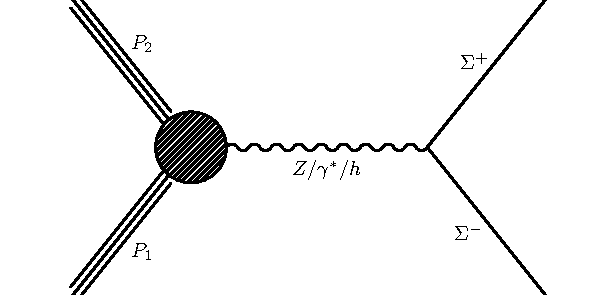
\includegraphics[width=.5\textwidth]{Introduction/SeesawProduction-SpSm}%
	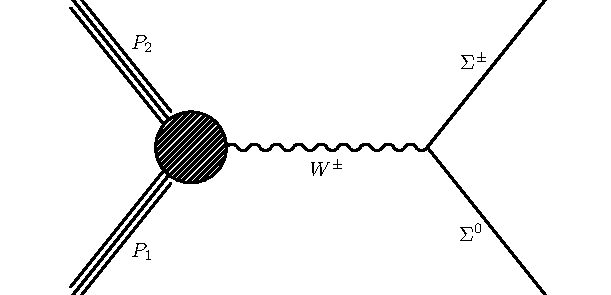
\includegraphics[width=.5\textwidth]{Introduction/SeesawProduction-SpmS0}
	\caption{Examples of Feynman diagrams for heavy fermion production in the type-III seesaw model.
	\label{fig:SeesawProduction}}
\end{center}
\end{figure}

We conduct a search for this signal by examining the final state with at least three electrons or muons. The primary decay channels of interest are $\Sigma^\pm \to \PW^\pm \nu$, $\Sigma^\pm \to \Z \ell^\pm$, $\Sigma^\pm \to \PH \ell^\pm$, $\Sigma^0 \to \PW^\pm \ell^\mp$, $\Sigma^0 \to \Z \nu$, $\Sigma^0 \to \PH \nu$, where $\ell = e, \mu$. Decays of $\Sigma^0 \Sigma^\pm$ and $\Sigma^+ \Sigma^-$ pairs result in 27 different production processes and can naturally lead to multilepton final states if several \PW\ or \Z\ bosons are involved, either directly or via a Higgs boson decay. An example Feynman diagram for one of the most relevant processes with three leptons in the final state, $\Sigma^\pm \Sigma^0 \to \PW^\pm \nu \PW^\pm \ell^\mp$ with leptonic $\PW^\pm$ decays, is shown in Fig.~\ref{fig:SeesawDecay}.
The decay rate of a $\Sigma$ to a given lepton $\ell$ is proportional to $v_{\ell N} = \frac{V_\ell}{\sqrt{|V_e|^2 + |V_\mu|^2 + |V_\tau|^2}}$. In the democratic scenario, the mixing parameters $V_\ell$ are the same for all the leptons.

\begin{figure}
\begin{center}
	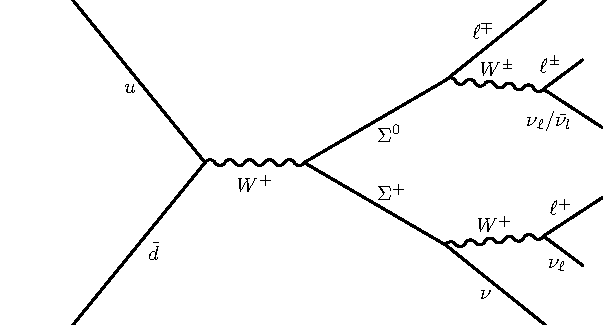
\includegraphics[width=.5\textwidth]{Introduction/Seesaw}
	\caption{Feynman diagram example of the fermion production and decay in the type-III seesaw model.
	\label{fig:SeesawDecay}}
\end{center}
\end{figure}


\subsection{Signal Model and Generation}
\label{sec:Samples/Signal}

We generate MC events to simulate all 27 production and decay mode combinations (see Sec.~\ref{sec:Introduction}). Generation for the model begins with a FeynRules Model file \cite{SeesawIII_Biggio}. Monte Carlo events are then generated in MadGraph5\_aMC@NLO \cite{Alwall:2011uj}. Bosonic decays are handled through Pythia 8, which is also in charge of hadronization \cite{Sjostrand:2007gs}. At the analysis level, we apply weights to correct for mismodeling of pile-up and \MET resolution.

The production cross sections were calculated with NLO + NLL accuracy using the CTEQ6.6 and MSTW2008nlo90cl parton distribution functions (PDFs) \cite{Fuks:2012qx,Fuks:2013vua}. Flavor-democratic values of the mixing angles are taken ($V_e = V_\mu = V_\tau = 10^{-6}$). This has no direct consequence on the fermion production cross section, but affects the branching ratios. The branching fraction of a heavy fermion to a lepton of flavor $\ell = e, \mu, \tau$ is proportional to $v_{\ell N} = \frac{V_\ell}{\sqrt{|V_e|^2 + |V_\mu|^2 + |V_\tau|^2}}$. Therefore, the flavor-democratic scenario gives $v_{\ell N} = \frac{1}{\sqrt{3}}$. The branching ratios from the pair-produced fermions to the bosonic level of the most relevant decay modes are given in Fig.~\ref{fig:SeesawBR}.

\begin{figure}
\begin{center}
	\includegraphics[width=.8\textwidth]{Theory/BR}
	\caption{Branching ratios from the pair-produced fermions to the bosonic level of the most relevant decay modes.
	\label{fig:SeesawBR}}
\end{center}
\end{figure}

\chapter[Experimental Apparatus]{Experimental Apparatus\protect\footnote{This chapter is largely taken from Ref.~\cite{Thomassen2012} (the author's Master's Thesis).}}
\label{chap:Detector}

\section{The Large Hadron Collider}
The particle collisions analyzed in the present thesis were generated by the Large Hadron Collider (LHC) which is located $100\,\unit{m}$ underground in the French--Swiss border area at the outskirts of Geneva \cite{1748-0221-3-08-S08001}. Several pre-accelerators are employed in order to accelerate the protons to different energies and to split them into bunches, before they reach the LHC ring (see Fig.~\ref{fig:LHC}) to form two beams traveling in opposite directions. In this ring of $26.7\,\unit{km}$ circumference, 1232 superconducting dipole magnets are used to produce a magnetic field of up to $8.33\,\unit{T}$ in order to accelerate the protons to their final center of mass energy of $\sqrt{s} = 13\,\TeV$.
%\footnote{The maximum design energy is $14\TeV$. LHC has been operating with increasing energies over the years, and it is planned to reach the design goal in 2014?.}
Additionally, about 7000 magnets are used for trajectory corrections and bunch focusing. Once the final velocity is reached, the protons are directed onto each other at certain points around the accelerator ring, where they collide. The collision products, in general, are not stable, but decay to intermediate and final state particles which are detected by large detector devices such as ATLAS or CMS. The bunch spacing is such that interactions are separated in time by $25\,\unit{ns}$.\footnote{However, several interactions might occur at the same time when two bunches meet. This phenomenon is referred to as ``pile-up'' and must be corrected for at analysis time, mostly by means of geometrical separation of the primary interaction vertex and by subtraction of expected pile-up contributions.}

The design luminosity of LHC is $10^{34}\,\unit{cm^{-2}s^{-1}}$. The instantaneous luminosity is given by
\begin{eqnarray}
	L = \frac{N_p^2 n_b f_\text{rev} \gamma_r}{4\pi \epsilon_n \beta*} F
\end{eqnarray}
where $N_b$ is the number of particles per bunch, $n_b$ is the number of bunches per beam, $f_\text{rev}$ is the revolution frequency, $\gamma_r$ is the relativistic gamma factor, $\epsilon_n$ is the normalized transverse beam emittance, $\beta*$ is the beta function at the collision point, and $F$ is the geometric luminosity reduction factor due to the crossing angle at the interaction point.

\begin{figure}
	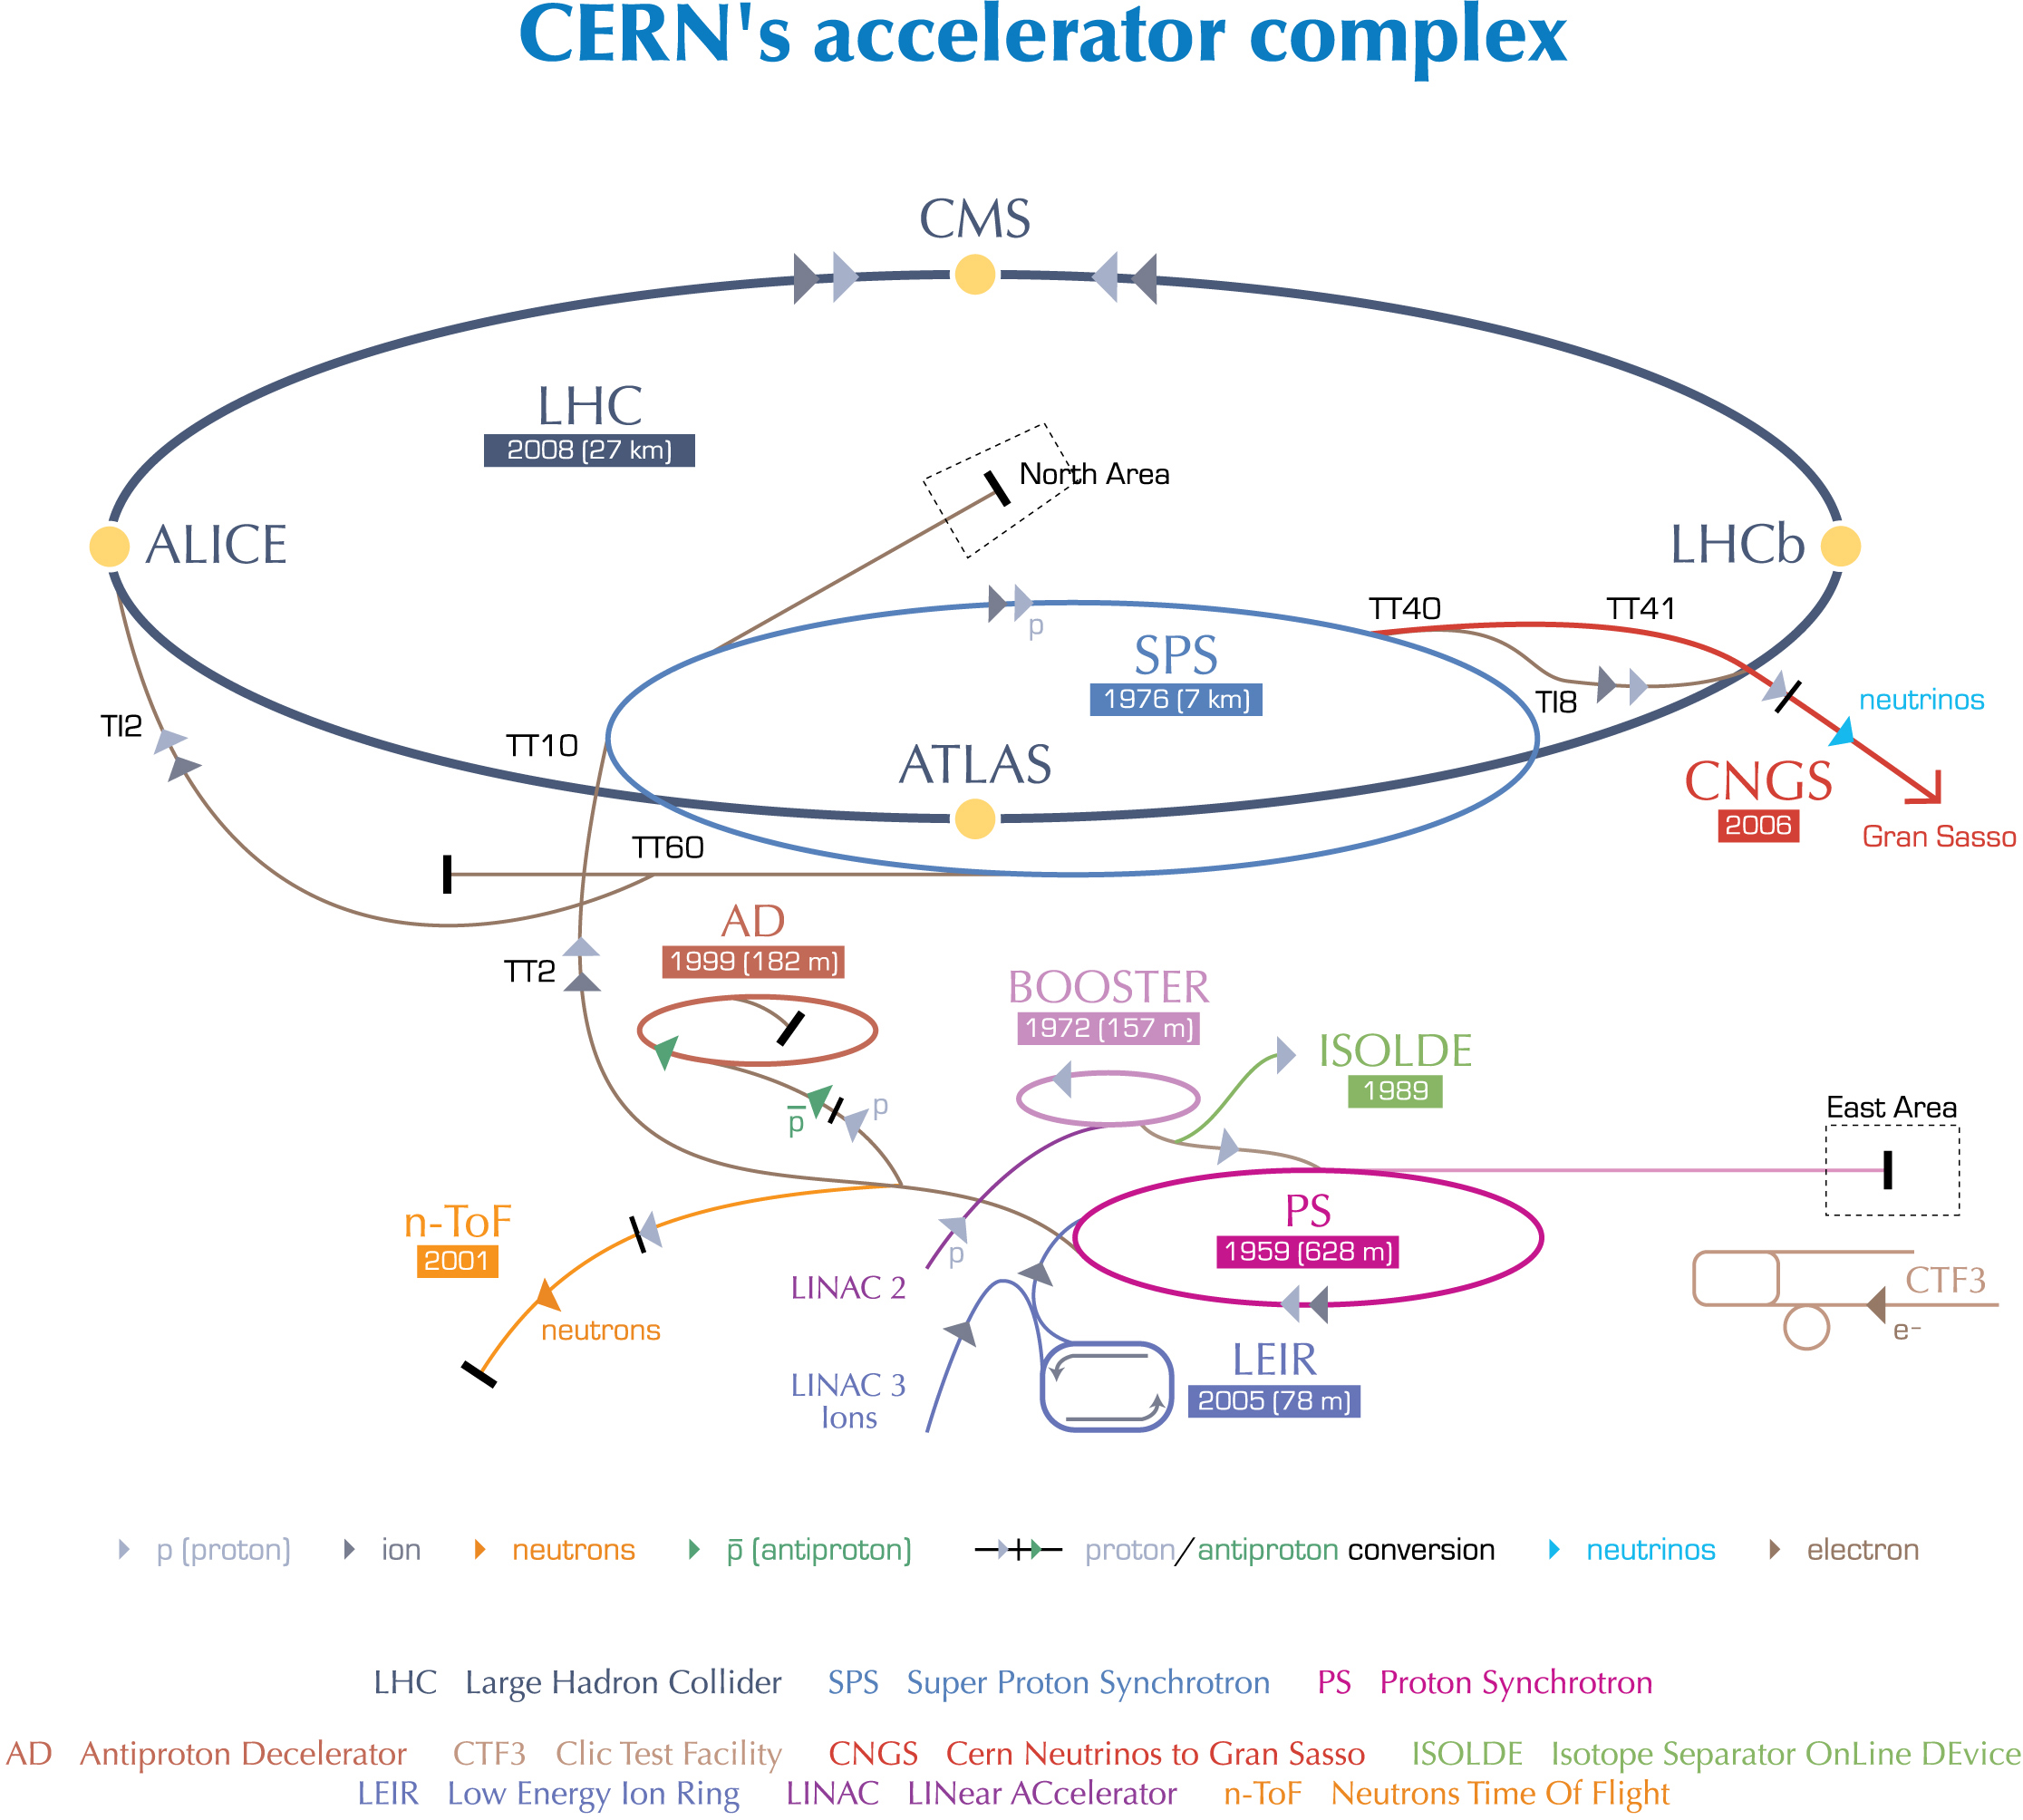
\includegraphics[width=.8\textwidth]{Detector/0812015}
	\centering
	\caption{CERN Accelerator Complex \cite{Christiane:1260465}. The diagram shows the different accelerators, detectors, and other facilities at CERN. For proton collisions, not all of the machinery is needed: Protons are initially accelerated to $50\MeV$ in a Linear Accelerator (LINAC~2). Then, they are transported to the Booster ($1.4\GeV$), to the Proton Synchrotron (PS, $25\GeV$) and the Super Proton Synchrotron (SPS, $450\GeV$) from where they are injected into LHC. The PS also takes care of arranging the protons in bunches with the correct spacing for LHC.}
	\label{fig:LHC}
\end{figure}

\section{The CMS Detector}
The Compact Muon Solenoid (CMS) is located at point 5 of the LHC accelerator ring and one of the two large, general purpose detector systems built at LHC. CMS consists of a large superconducting solenoid which contains a silicon-based tracker, an electromagnetic calorimeter made of scintillating lead-tungstate crystals, and a brass-based scintillating hadron calorimeter (see Fig.~\ref{fig:CMS}); the total weight is about 12500 tons \cite{Chatrchyan:2008zzk}. A special feature of CMS is its superconducting solenoid of $6\,\unit{m}$ internal diameter which creates a strong magnetic field ($3.8\,\unit{T}$) that is suitable for high precision measurements of charged particles at very high energies.

\begin{figure}
	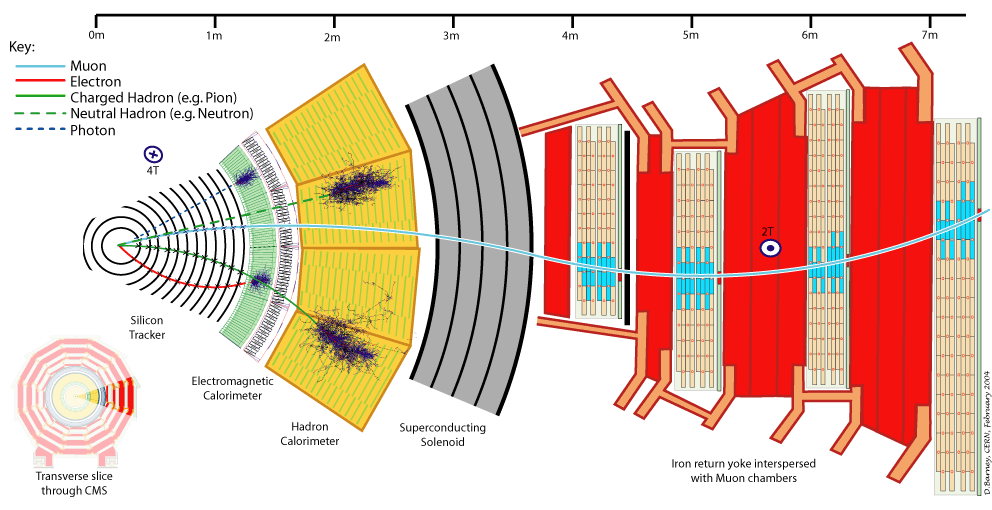
\includegraphics[width=\textwidth]{Detector/CMS_Slice}
	\centering
	\caption{A transverse slice through CMS \cite{CMS_Slice}. The illustration shows the most important detector components as well as examples of different particles as they are detected while traveling through the detector.}
	\label{fig:CMS}
\end{figure}

In order to describe the properties of particles observed in collision events, a coordinate system is defined. The origin is declared where the main interaction point is expected to occur. The $x$ axis points radially towards the center of the LHC, the $y$ axis points in the upward direction, and together with the $z$ axis that points along the beampipe (counterclockwise), a right-handed coordinate system is constructed. In cylindrical coordinates, the $z$ axis is the same, and $\phi$ is the azimuthal angle. Starting from the positive $z$ axis, the polar angle $\theta$ increases towards the center of the LHC. Since the polar angle $\theta$ is not Lorentz-invariant, the pseudorapidity $\eta$ is defined as a Lorentz-invariant alternative coordinate,\footnote{This quantity is the massless limit of the rapidity which is an additive measure of relativistic velocity and defined as $\log \frac{E + p_z}{E - p_z}$.}
\begin{eqnarray}
	\eta = - \log \tan \frac{\theta}{2}.
\end{eqnarray}
When the directional separation between particles needs to be determined,
\begin{eqnarray}
	\Delta R = \sqrt{(\Delta \eta)^2 + (\Delta \phi)^2}
\end{eqnarray}
comes in handy as a measure of two particles' separation in $\eta$ and $\phi$.

The following sections are concerned with the individual detector components used for the measurement of the particle properties that are recorded from collision events, along the lines of Ref.~\cite{Xie:1455454}.

\subsection{Tracking System}
In order to precisely reconstruct the path of charged particles in CMS, a tracking system based on silicon-based p--n junctions was installed. A high reverse-bias voltage is applied across the junction, creating a depletion zone with an electric field. When a charged particle passes this zone, it ionizes the silicon atoms, and the resulting electrons are free to move and create an electrical current which is detected. By setting up several layers containing a large number of such p--n junctions with small dimensions, a highly sensitive tracking device can be created. In total, 15400 tracking sensors are installed in CMS and operated at low temperature in order to minimize the effects of radiation damage. The CMS tracking system consists of several parts:

\subsubsection*{Pixel Detector}
The Pixel Detector is located within $10\,\unit{cm}$ from the $z$ axis and is used to account for small displacements close to the primary vertex, To keep the occupancy per bunch crossing reasonably low, a pixel size of $100\,\mum \times 150\,\mum$ is used. The spatial resolution is $10\,\mum$ to $20\,\mum$.

\subsubsection*{Strip Detector}
The Strip Detectors are located both in the barrel as well as in the endcap regions of CMS. In either case, several layers of silicon strips are placed behind each other to provide similar functionality as in the case of the pixel detector. The dimensions are much wider than those of the pixels. In each detector region, they are chosen according to the corresponding production characteristics such that the occupancy will not be too high, so that a hit will provide informative value.

\subsection{Electromagnetic and Hadronic Calorimeter}
The calorimetry system is designed to measure the energies of incident particles. Depending on the particle type, the energy is deposited in different parts of the system \cite{EvaHalkiadakis}:

\begin{figure}
	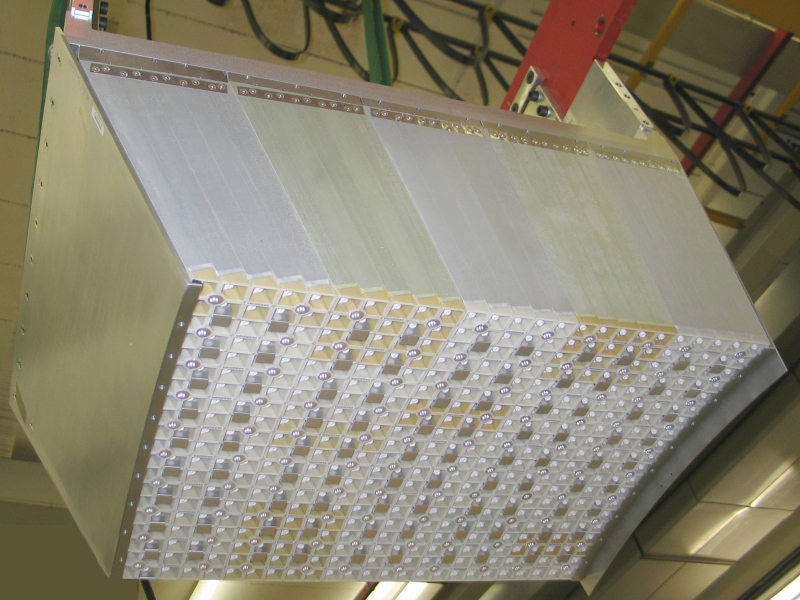
\includegraphics[width=.7\textwidth]{Detector/ECAL_crystal}
	\centering
	\caption{A module of the electromagnetic calorimeter consisting of 500 lead-tungstate crystals.}
	\label{fig:ECAL}
\end{figure}

\subsubsection*{Electromagnetic Calorimeter (ECAL)}
The task of the ECAL is to measure the energy of charged particles (especially electrons) and photons. The lead-tungstate (PbWO$_4$) material of the crystals is very dense, but optically transparent; a module is shown in Fig.~\ref{fig:ECAL}. When electrons or photons travel through, they lose energy in a cascade process due to bremsstrahlung and ionization (electrons) and $e^+ e^-$ pair production (photons). In addition, the crystals are excited so that they produce light from scintillation which is detected by photodetectors and used to infer the incident particle's energy.

In the barrel ($|\eta| \leq 1.479$), there are 61200 crystals with front face dimensions of $22\,\unit{mm} \times 22\,\unit{mm}$, covering 0.0174 in both $\eta$ and $\phi$, and a length of $230\,\unit{mm}$, corresponding to about 25 radiation lengths. In the endcap ($1.479 \leq |\eta| \leq 3.0$), there are 7324 crystals with a surface area of $28.6\,\unit{mm} \times 28.6\,\unit{mm}$ and a length of $220\,\unit{mm}$. An additional preshower detector is installed in front of the endcap component that helps distinguishing photons from neutral pions. This setup covers the $\eta$ range up to the forward region without any gaps.

\subsubsection*{Hadronic Calorimeter (HCAL)}
Like the ECAL, the HCAL is for the most part located inside the solenoid. While the ECAL is a homogeneous, the HCAL is a sampling calorimeter which means that it consists of alternating layers of an active, signal-generating medium, and a passive medium whose only purpose is to absorb energy. The active material is a plastic scintillator which is $3.7\,\unit{mm}$ thick and organized in a tile pattern. The scintillation light emitted in a certain $\eta$--$\phi$ cell is summed up optically, forming a ``tower'', collected by wavelength-shifting fibers, and channeled to hybride photodiodes.

The barrel part ($|\eta| \leq 1.4$) has 2304 towers, each covering 0.087 in $\eta$ and $\phi$. There are 15 absorption layers, mostly made from brass. To increase accuracy, a number of layers is placed at the outside of the magnet coil (Hadron Outer, HO). The endcap parts cover the region $1.3 \leq |\eta| \leq 3.0$ with 19 layers of active scintillating material, covering cell of width $5^\circ$ to $10^\circ$ in $\phi$ and 0.35 to 0.09 in $\eta$. In the very forward region ($3.0 \leq |\eta| \leq 5.0$), a fourth HCAL part (Hadron Forward, HF) consisting of an active quartz fiber medium and steel absorbers is located. The quartz fiber material emits Čerenkov light that is detected by photomultipliers with resolution 0.175 in $\eta$ and $10^\circ$ in $\phi$.

\subsection{Muon System}
The muon is about 200 times as heavy as the electron. Since the bremsstrahlung-induced dissipation in the calorimeter is proportional to $\text{mass}^{-2}$ \cite{bock2013particle}, it is suppressed by a factor of 40000. Therefore, muons can easily traverse the calorimeter system, so that other more specialized detector systems can be employed outside the calorimeter.

In the barrel, 250 drift tube (DT) chambers are used to identify muons. Four shells of stations are located at different distances from the $z$ axis, embedded in the return yoke of the solenoid (see Fig.~\ref{fig:muonSystem}). In the endcap, 468 cathode strip chambers (CSC) are arranged in concentric rings, most of them containing 36 CSCs. Charged particles travelling through the gas inside a CSC cause ionization, followed by a charged avalanche whose distribution is measured on the cathode plane. From this information, it is possible to reconstruct the track geometry. Each of the DT and CSC stations is accompanied by resistive plate chambers that are used for precise timing and velocity determination.

\begin{figure}
	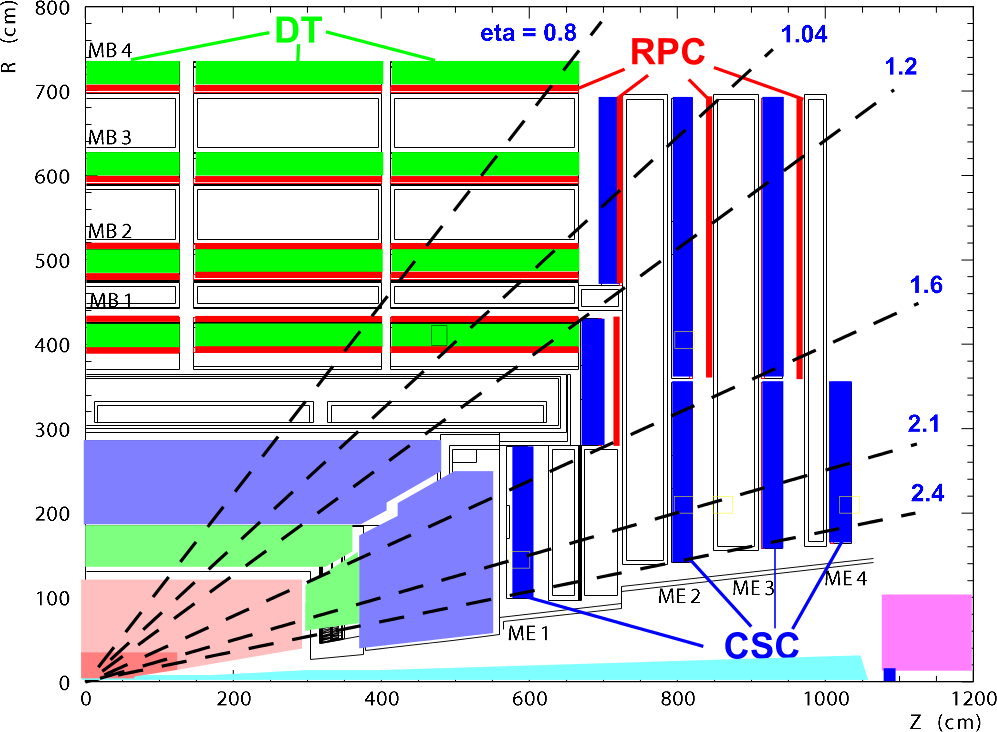
\includegraphics[width=\textwidth]{Detector/muon}
	\centering
	\caption{Sketch of the muon system in CMS in $r$--$z$ view. The drift tubes are displayed in dark-green, the cathode strip chambers in dark-blue, and the resistive plate chambers in dark-red. The light-colored areas are the tracker and calorimeter. The interaction point is located at the origin of the coordinate system.}
	\label{fig:muonSystem}
\end{figure}

\subsection{Trigger and Data Storage}
LHC performs about about $10^7$--$10^8$ proton--proton collisions per second. Since not all events can be stored (about $300\,\text{Hz}$), a rejection rate of about $10^5$ is required. First-level decisions are reached by the Level-1 (L1) trigger system which performs quick assessments of events within about 1\mus while the event data, about $0.5\,\text{MB}$ each, is held in buffers. Potentially interesting events are then forwarded to a dedicated computing farm where high-level triggers (HLT) run more precise reconstruction algorithms in order to decide which events should be kept.

Finally, accepted events are transmitted to the storage manager system which arranges the subsequent transfer to the permanent Tier-0 storage systems located at the CERN main site and at the Wigner Research Centre for Physics in Budapest (Hungary). From there, data is distributed to interested Tier-1 and Tier-2 sites across the globe for analysis purposes. Petabyte-range storage systems are employed world-wide to manage the large amounts of data that are used on a daily basis.

\chapter{Search Strategy}
\label{chap:Strategy}

\section{General Approach}
\label{sec:Strategy/general}

Candidate events in this search must have a total of at least three leptons, each of which can be either an electron or a muon. We classify multilepton events into search channels on the basis of the number of leptons, lepton flavor, lepton relative charges, charge and flavor combinations, and other kinematic quantities described below.

We classify each event in terms of the maximum number of opposite-sign same-flavor (OSSF) dilepton pairs that can be made by using each lepton only once. For example, both $\mu^+\mu^-\mu^-$ and $\mu^+\mu^-e^-$ are OSSF1, $\mu^+\mu^+e^-$ is OSSF0, and $\mu^+\mu^-e^+e^-$ is OSSF2. We denote a lepton pair of different flavors as $\ell\ell^\prime$.

We classify events as containing a leptonically-decaying \Z if at least one OSSF pair has $m_{\ell^+\ell^-}$ in the \Z mass window $(91 \pm 10)\GeV$. For $m_{\ell^+\ell^-}$ outside the \Z boson mass window, events are separated into bins below and above the \Z mass window. We refer to these three mass ranges as ``on-\Z'', ``below-\Z'', and ``above-\Z''.

In cases of ambiguity (such as $\mu^+\mu^-\mu^-$ with one pair below and one pair above \Z), we need to pick a specific pair. We compare two methods:
\begin{enumerate}
	\item Choose the pair whose invariant mass is closest to the \Z mass.
	\item Choose the pair closest to the \Z mass, with the additional condition that pairs above the \Z window are not considered if there is a pair below the \Z window (thus shifting events from above-\Z to below-\Z).
\end{enumerate}
Fig.~\ref{fig:app:Zbinning} shows that there is little difference between both approaches. Nevertheless, we take the second approach to achieve a more separative categorization of background, especially around the high end of the \Z window.
\begin{figure}
\begin{center}
	\begin{subfigure}[b]{.7\textwidth}
		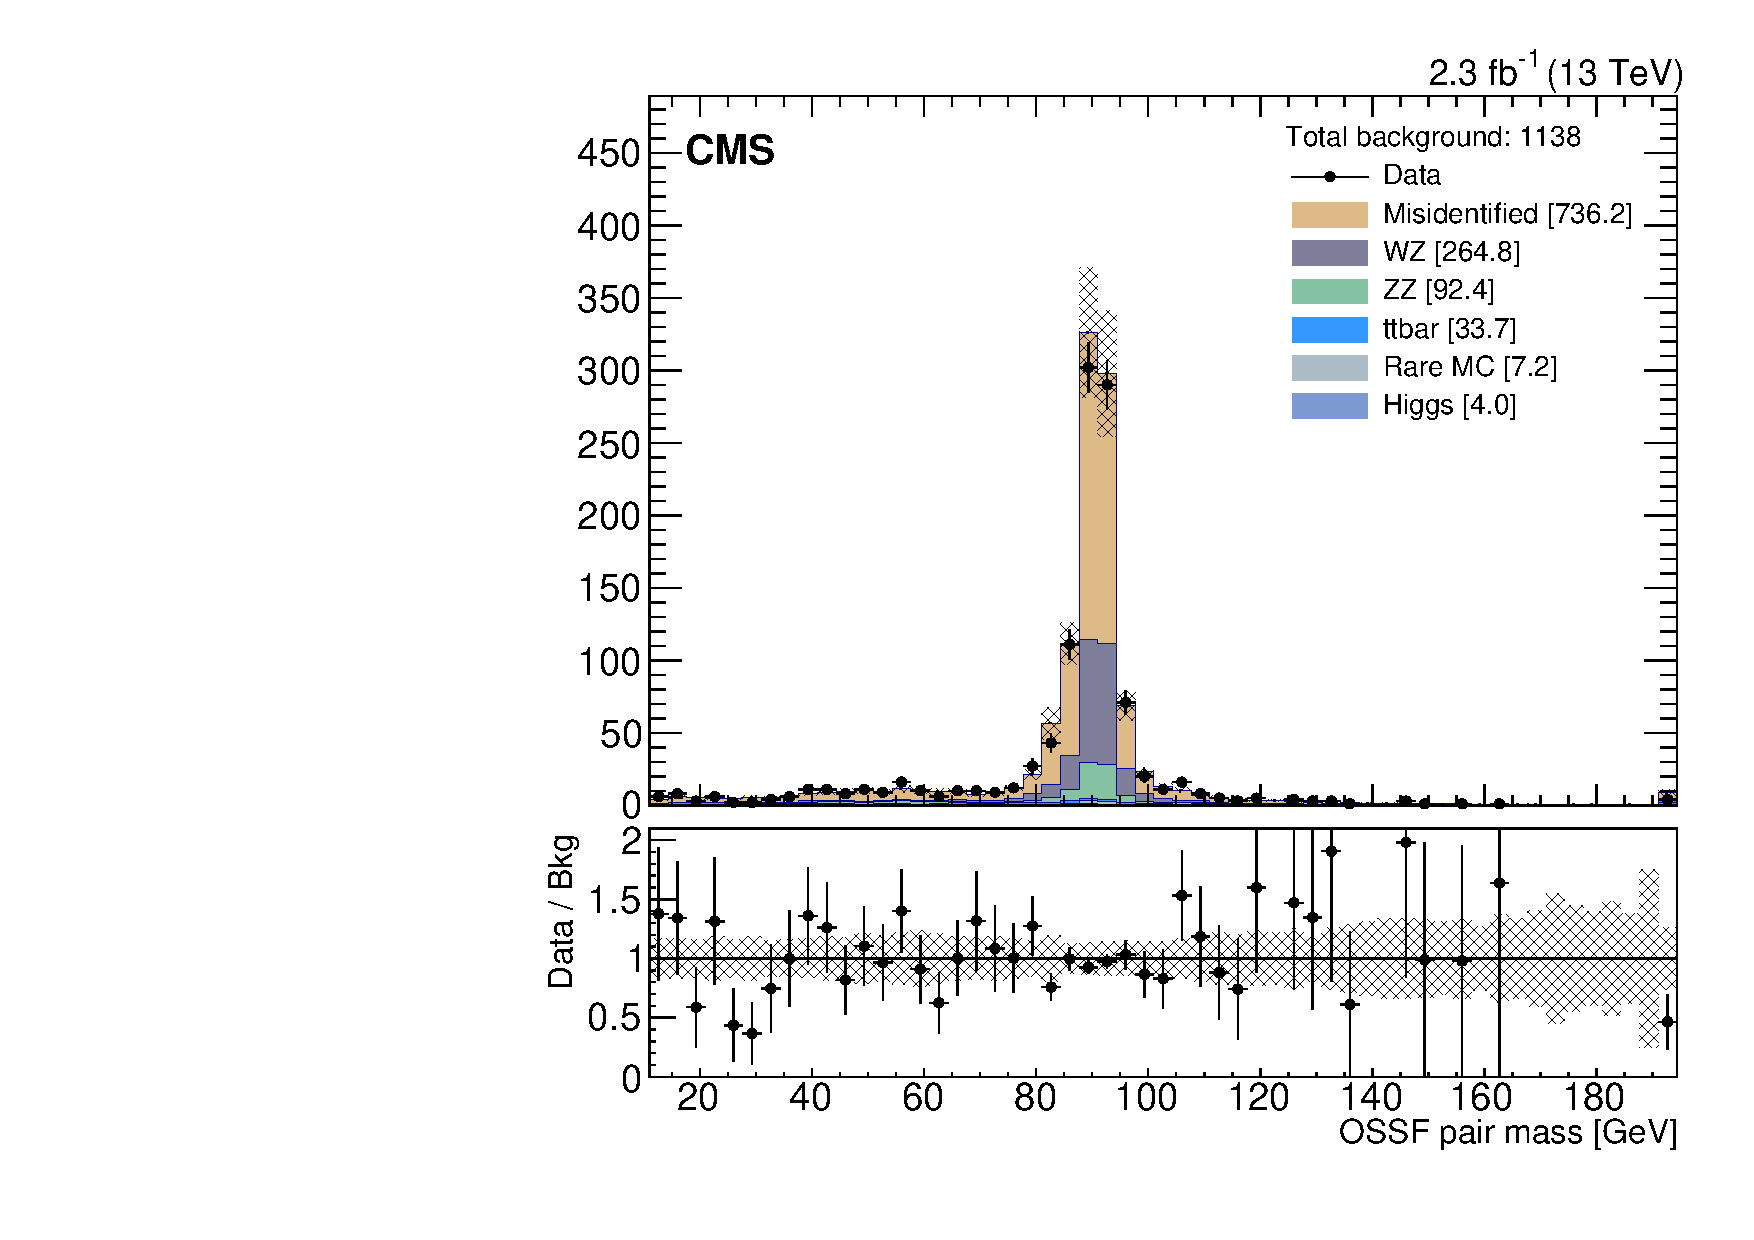
\includegraphics[width=\textwidth]{Strategy/Z_L3MET0to50_noAIC_OSSFCLOSEMLL}%
		\caption{method 1}
	\end{subfigure}
	\begin{subfigure}[b]{.7\textwidth}
		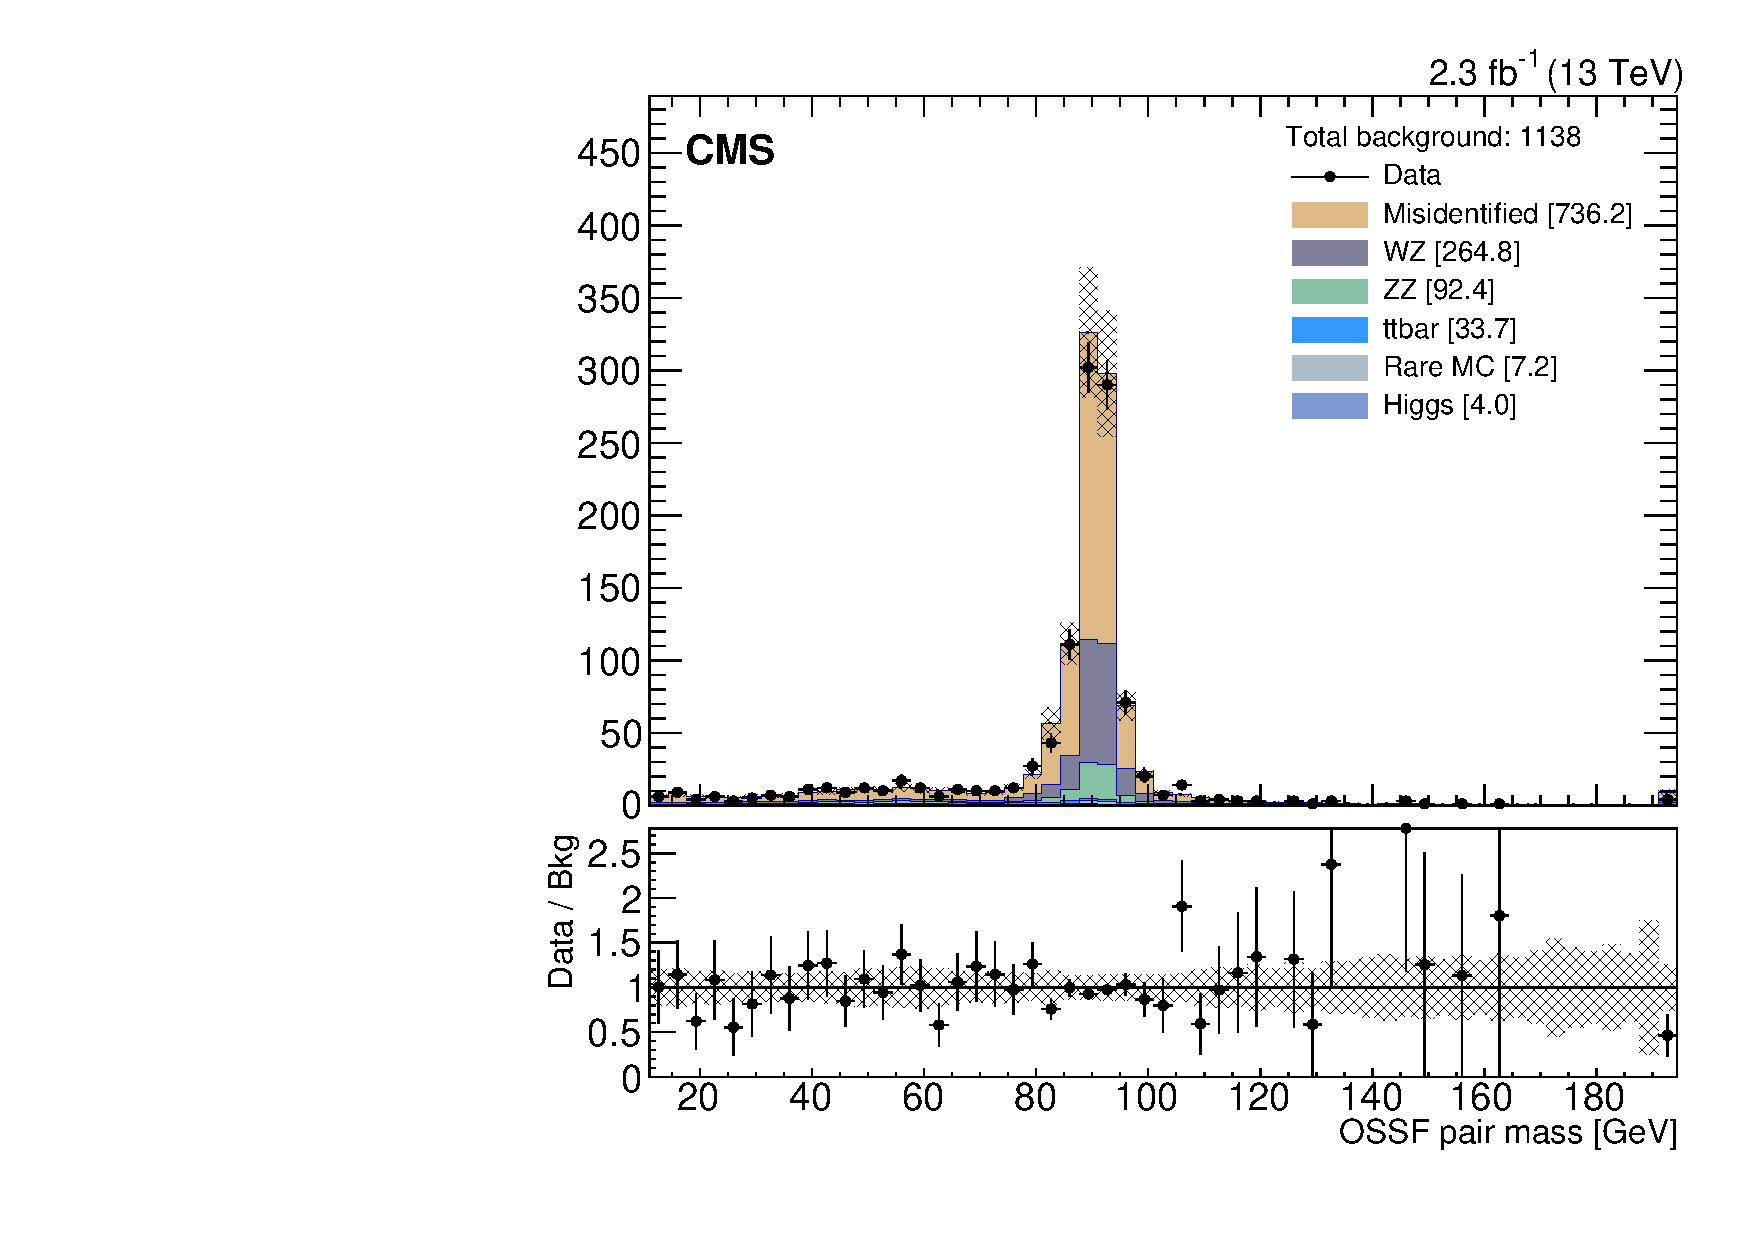
\includegraphics[width=\textwidth]{Strategy/Z_L3MET0to50_noAIC_MOSSF}
		\caption{method 2}
	\end{subfigure}
	\caption{$m_{\ell\ell}$ distribution in in the dilepton fake region (off-\Z, trilepton events with $m_{\ell\ell\ell}$ on \Z have been vetoed).
	\label{fig:app:Zbinning}}
\end{center}
\end{figure}

The most important multilepton background processes are \WZ, \Z or \ttbar events in which there is a misidentified lepton, and \ZZ production. In addition, there are various rare background processes like WWZ or $\ttbar\PW$. However, the level of SM background varies considerably across channels; for example, channels containing OSSF pairs suffer from larger backgrounds than do channels with OSSF0. Hence, all these charge combinations are considered as different channels.

%Backgrounds can be tamed by binning in appropriate quantities. Since the signal leptons have relatively high \pt and since in some decay modes there is missing transverse energy (\MET) from accompanying neutrinos, we find that binning in $L_\textrm{T} + \MET$, where $L_\textrm{T}$ is the scalar sum of the lepton \pt's, separates the signal from the background. We find that lepton \pt binning alone gives about 20\,\% worse signal-to-background ratios in the most sensitive signal regions.
%Additional separation is achieved through the on- and off-\Z binning described above.

\section{Signal Regions}
\label{sec:Optimization}

%The type-III seesaw signal comes both with 3 and 4 (or more) leptons as well as with and without OSSF pairs, which in turn may have an invariant mass that is compatible with \Z production. This lays the foundation for our binning scheme.

Backgrounds can be tamed by binning in appropriate quantities. Given the relatively high signal lepton momenta due to the large masses of the parent particles, cutting on $L_\textrm{T}$, the scalar lepton \pt sum, may be a good idea. This is especially true for decay modes like $\Sigma^\pm \to \ell^\pm \Z \to \ell^\pm ~ \ell^{\prime \pm} \ell^{\prime \mp}$ where the heavy fermion mass is transformed into the lepton momenta. However, such an $L_\textrm{T}$ cut acts at the expense of the signal efficiency in other modes like $\Sigma^0 \to \PH \nu \to \PW\PW\nu$, where lepton \pt's are somewhat lower because the intermediate bosons may be off-shell, and the neutrinos carry away some of the momentum that appears as missing transverse energy (\MET). However, we can still achieve high efficiency by using $L_\textrm{T} + \MET$ instead, which we found suitable for signal selection for both of the described channel types (Fig.~\ref{fig:Optimization2}). The background rejection effectiveness of this variable is shown in Fig.~\ref{fig:Optimization}. We find that lepton \pt binning alone gives about 20\,\% worse signal-to-background ratios in the most sensitive signal regions.

\begin{figure}
\begin{center}
	\begin{subfigure}[b]{.7\textwidth}
		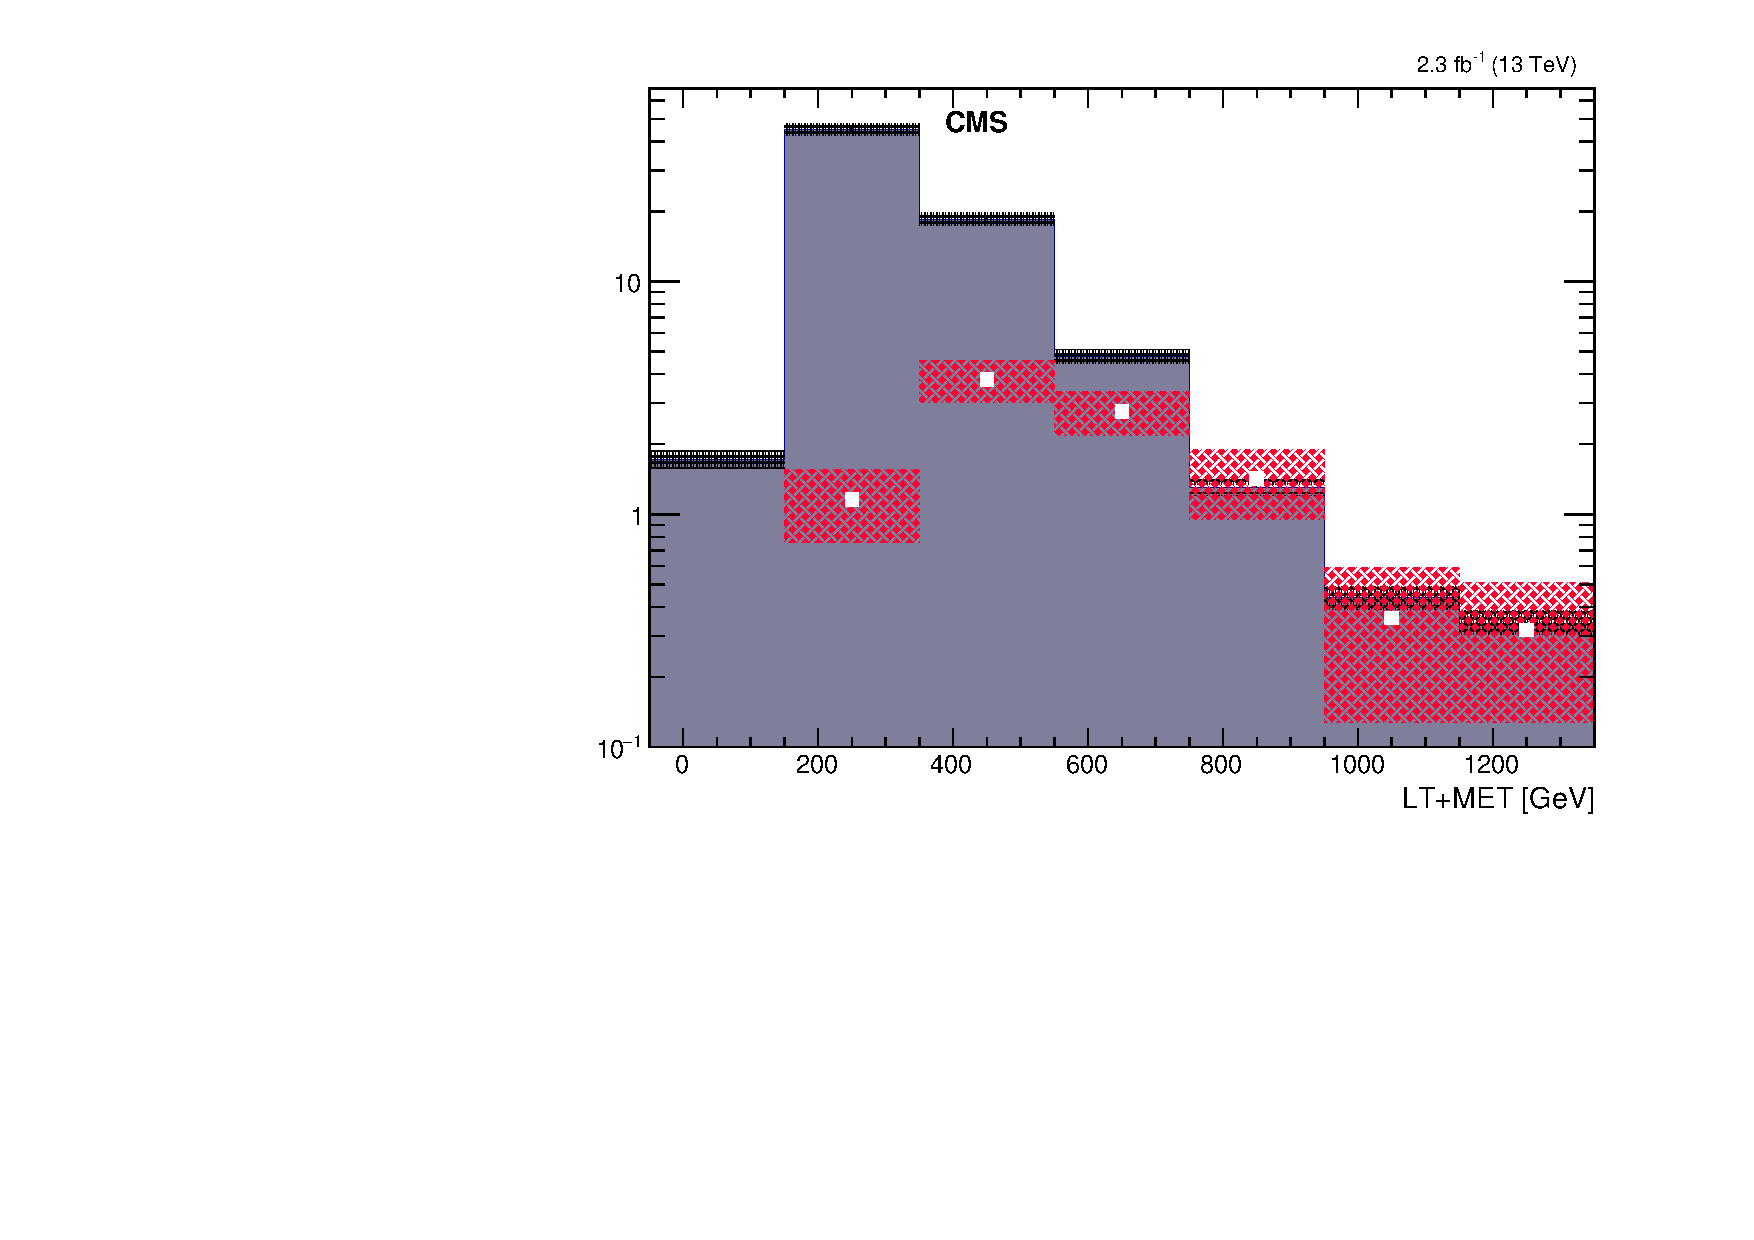
\includegraphics[width=\textwidth]{Strategy/LT+MET_tr+w+vltr0wl}
		\caption{$\Sigma^+ \to \PW^+ \nu, \Sigma^0 \to \PW^\pm \ell^\mp$}
	\end{subfigure}
	\begin{subfigure}[b]{.7\textwidth}
		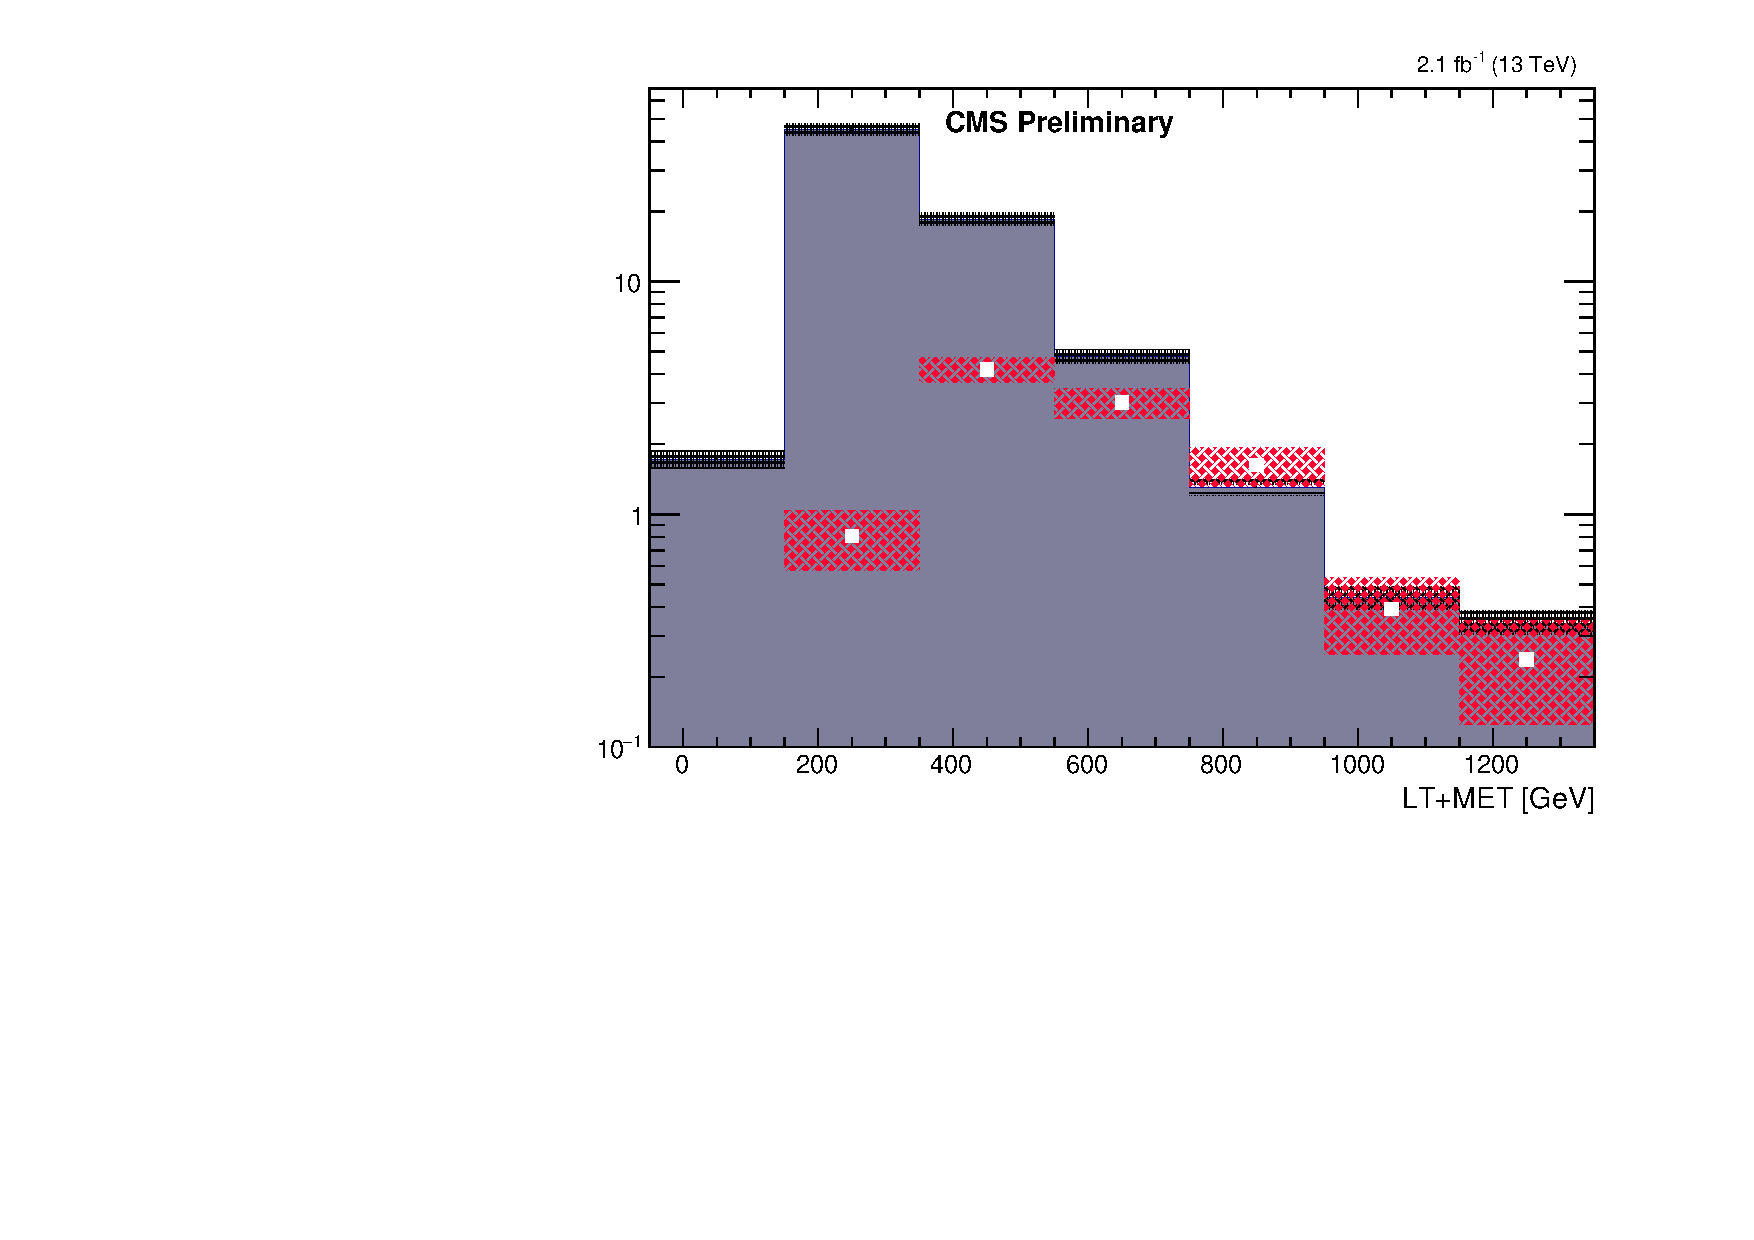
\includegraphics[width=\textwidth]{Strategy/LT+MET_tr+zl+tr-zl-}
		\caption{$\Sigma^+ \to Z \ell^+, \Sigma^- \to Z \ell^-$}
	\end{subfigure}
	\caption{$L_\textrm{T} + \MET$ shape for two different production and decay modes at $m_\Sigma = 340\GeV$, with \WZ background. Signal normalization arbitrary (for illustration purposes only).
	\label{fig:Optimization2}}
\end{center}
\end{figure}

\begin{figure}
\begin{center}
	\includegraphics[width=.7\textwidth]{Strategy/LT+MET}
	\caption{$L_\textrm{T} + \MET$ distribution after event selection cuts from Sec.~\ref{sec:Selection}, to illustrate the signal separation power of this variable (last bin includes overflow). Backgrounds are described in Chapter~{\ref{chap:Backgrounds}}. The signal ($m_\Sigma = 420\GeV$, sum of all production and decay modes) is shown as white square dots with a pink hashed uncertainty band. The background uncertainty is specified by the gray band. Uncertainty bands include both statistical and systematic uncertainties. Numbers in square brackets denote the number of events contributed by each process.
	\label{fig:Optimization}}
\end{center}
\end{figure}

The optimum requirement on $L_\textrm{T} + \MET$ depends on the mass of the heavy fermions. In order to separate the signal as well as possible from the background, we categorize the data in bins of $L_\textrm{T} + \MET$, regardless of the particle mass. We use 4 bins of width 200\GeV starting at 350\GeV, plus an overflow bin. Below 350\GeV, the amount of signal is insignificant in comparison to the background.

We remove any overlap with background control regions by explicitly vetoing the control region selections. Furthermore, we discard the below-\Z trilepton region and the four-lepton region without an OSSF pair because, with the given amount of luminosity, they contain a neglibile amount of signal and thus do not contribute to the sensitivity.

As a result, we have four $L_\textrm{T} + \MET$ distributions, depending on the lepton properties: 3 leptons without OSSF pair, 3 leptons with OSSF pair on-\Z, 3 leptons with OSSF pair above-\Z, and 4 leptons with at least one OSSF pair. Each distributions begins at 350\GeV and reaches to 1150\GeV in steps of 200\GeV. We add an overflow bin for $L_\textrm{T} + \MET > 1150\GeV$ so that that there are five bins per distribution. The resulting set of 20 signal regions is described in Table~\ref{tab:SR}.

\begin{table}
\centering
\caption{Signal Regions. Overlap with control regions removed everywhere.} \label{tab:SR}
\begin{tabular}{c l c }
\hline\hline
$n_\textrm{leptons}$ & OSSF pair & $L_\textrm{T} + \MET$ [GeV]\\
\hline
3 & & \\
 & none & \multirow{3}{*}{\rotatebox{9}{350..1150 in steps of 200, plus overflow}} \\
 & on-\Z & \\
 & above-\Z & \\
\hline
$\geq 4$ & $\geq 1$ & 350..1150 in steps of 200, plus overflow \\
\end{tabular}
\end{table}

\section{Signal Regions}
\label{sec:Optimization}

%The type-III seesaw signal comes both with 3 and 4 (or more) leptons as well as with and without OSSF pairs, which in turn may have an invariant mass that is compatible with \Z production. This lays the foundation for our binning scheme.

Backgrounds can be tamed by binning in appropriate quantities. Given the relatively high signal lepton momenta due to the large masses of the parent particles, cutting on $L_\textrm{T}$, the scalar lepton \pt sum, may be a good idea. This is especially true for decay modes like $\Sigma^\pm \to \ell^\pm \Z \to \ell^\pm ~ \ell^{\prime \pm} \ell^{\prime \mp}$ where the heavy fermion mass is transformed into the lepton momenta. However, such an $L_\textrm{T}$ cut acts at the expense of the signal efficiency in other modes like $\Sigma^0 \to \PH \nu \to \PW\PW\nu$, where lepton \pt's are somewhat lower because the intermediate bosons may be off-shell, and the neutrinos carry away some of the momentum that appears as missing transverse energy (\MET). However, we can still achieve high efficiency by using $L_\textrm{T} + \MET$ instead, which we found suitable for signal selection and background rejection for both of the described channel types. The effectiveness of this variable is shown in Fig.~\ref{fig:Optimization}. We find that lepton \pt binning alone gives about 20\,\% worse signal-to-background ratios in the most sensitive signal regions.

\begin{figure}
\begin{center}
	\includegraphics[width=.7\textwidth]{Optimization/LT+MET}
	\caption{$L_\textrm{T} + \MET$ distribution after event selection cuts from Sec.~\ref{sec:Selection}, to illustrate the signal separation power of this variable (last bin includes overflow). Backgrounds are described in Sec.~{\ref{sec:backgrounds}}. The signal ($m_\Sigma = 420\,\GeV$, sum of all production and decay modes) is shown as white square dots with a pink hashed uncertainty band. The background uncertainty is specified by the gray band. Uncertainty bands include both statistical and systematic uncertainties. Numbers in square brackets denote the number of events contributed by each process.
	\label{fig:Optimization}}
\end{center}
\end{figure}

The optimum requirement on $L_\textrm{T} + \MET$ depends on the mass of the heavy fermions. In order to separate the signal as best as possible from the background, we categorize the data in bins of $L_\textrm{T} + \MET$, regardless of the particle mass. We use 4 bins of width 200\,\GeV starting at 350\,\GeV, plus an overflow bin. Below 350\,\GeV, the amount of signal is insignificant in comparison to the background.

We remove any overlap with background control regions by explicitly vetoing the control region selections. Furthermore, we discard the below-\Z trilepton region and the four-lepton region without an OSSF pair because, with the given amount of luminosity, they contain a neglibile amount of signal and thus do not contribute to the sensitivity.

As a result, we have four $L_\textrm{T} + \MET$ distributions, depending on the lepton properties: 3 leptons without OSSF pair, 3 leptons with OSSF pair on-\Z, 3 leptons with OSSF pair above-\Z, and 4 leptons with at least one OSSF pair. Each distributions begins at 350\,\GeV and reaches to 1150\,\GeV in steps of 200\,\GeV. We add an overflow bin for $L_\textrm{T} + \MET > 1150\,\GeV$ so that that there are five bins per distribution, giving a total of 20 signal regions.

%The resulting set of 20 signal regions is described in Table~\ref{tab:SR}.

%\begin{table}[h]
%\centering
%\caption{Signal Regions. Overlap with control regions removed everywhere.} \label{tab:SR}
%\begin{tabular}{c l c }
%\hline\hline
%$n_\textrm{leptons}$ & OSSF pair & $L_\textrm{T} + \MET$ [GeV]\\
%\hline
%3 & & \\
% & none & \multirow{3}{*}{\rotatebox{9}{350..1150 in steps of 200, plus overflow}} \\
% & on-\Z & \\
% & above-\Z & \\
%\hline
%$\geq 4$ & $\geq 1$ & 350..1150 in steps of 200, plus overflow \\
%\end{tabular}
%\end{table}

\chapter{Triggers and Object Selection}
\label{sec:ObjectID}

The data for this search are collected using several dilepton triggers. The double electron trigger requires two electrons with \pt thresholds of 17\,\GeV on the leading electron and 12\,\GeV on the sub-leading electron. The double muon trigger requires two muons with \pt thresholds of 17 and 8\,\GeV on the leading and sub-leading muons, respectively. We use two muon/electron cross triggers, one of which requires a 17\,\GeV muon and a 12\,\GeV electron, while the other requires a 17\,\GeV electron and a 8\,\GeV muon.

Events that pass the trigger are required to satisfy additional selection criteria. Electrons with $\pt \geq 7\,\GeV$ and $|\eta| \leq 2.5$ as well as muons with $\pt \geq 5\,\GeV$ and $|\eta| \leq 2.4$ are reconstructed using the particle-flow (PF) algorithm which utilizes measured quantities from the tracker, calorimeter, and muon system \cite{CMS-PAS-PFT-09-001}. The matching candidate tracks must satisfy quality requirements and spatially match with the energy deposits in the ECAL and the tracks in the muon detectors, as appropriate.

Sources of background leptons include genuine leptons occurring inside or near jets, hadrons that punch through into the muon system and are misidentified as muons, hadronic showers with large electromagnetic fractions, or photon conversions. An isolation requirement -- imposing a selection based on the size of the lepton transverse momentum in comparison to the transverse momenta of other particles in its immediate neighborhood -- strongly reduces the background from misidentified leptons, since most of them occur inside jets. In this search, we use the multi-isolation variable which features a \pt-dependent isolation cone and pile-up correction \cite{CMS-PAS-SUS-15-008}. For electrons, the medium working point is employed, while for muons, we use the tight working point. Further details on the input variables, working points, and their efficiencies can be found in \cite{CMS-PAS-SUS-15-008}.

The signal leptons originate from the interaction point. After the isolation selection, the most significant background sources are residual non-prompt leptons from heavy quark decays, where the lepton tends to be more isolated because of the high \pt with respect to the jet axis. This background is reduced by requiring that the leptons satisfy $d_\textrm{z} \leq 0.1\,\cm$ where $d_\textrm{z}$ is the longitudinal impact parameter with respect to the primary interaction vertex, and that the impact parameter $d_\textrm{xy}$ between the track and the event vertex in the plane transverse to the beam axis be small: $d_\textrm{xy} \leq 0.05\,\cm$. The isolation and impact parameter criteria retain signal but significantly reject misidentified leptons.

The missing transverse momentum is calculated as the negative vectorial sum of the transverse momenta of all the PF candidates. The missing transverse energy \MET is defined as the magnitude of this vector. Jet energy corrections are applied to all jets and also propagated to the calculation of \MET \cite{CMS-PAS-JME-12-002}. We apply additional smearing to simulation samples to model the \MET resolutions we find in data as a function of jet activity and number of interaction vertices in an event.

\chapter{Event Selection}
\label{sec:Selection}

For the three leading leptons, we apply offline thresholds of 20, 15, 10\,\GeV. We find that with these thresholds, the trigger efficiency of trilepton events is close to 100\%.

Events with an opposite-sign lepton pair with mass below 12 GeV are vetoed to reduce background from low-mass resonances. Furthermore, we reject trilepton events with an OSSF pair below the \Z boson mass window when the trilepton mass is within the \Z mass window. This cuts away background from asymmetric photon conversions in $\Z \to \ell\ell^* \to \ell\ell\gamma$, where the photon converts into two additional leptons, one of which is lost.

\chapter{Signal Model and Generation}
\label{sec:Samples/Signal}

We generate MC events to simulate all 27 production and decay mode combinations (see Sec.~\ref{sec:Introduction}). Generation for the model begins with a FeynRules Model file \cite{SeesawIII_Biggio}. Monte Carlo events are then generated in MadGraph5\_aMC@NLO \cite{Alwall:2011uj}. Bosonic decays are handled through Pythia 8, which is also in charge of hadronization \cite{Sjostrand:2007gs}. At the analysis level, we apply weights to correct for mismodeling of pile-up and \MET resolution.

The production cross sections were calculated with NLO + NLL accuracy using the CTEQ6.6 and MSTW2008nlo90cl parton distribution functions (PDFs) \cite{Fuks:2012qx,Fuks:2013vua}. Flavor-democratic values of the mixing angles are taken ($V_e = V_\mu = V_\tau = 10^{-6}$). This has no direct consequence on the fermion production cross section, but affects the branching ratios. The branching fraction of a heavy fermion to a lepton of flavor $\ell = e, \mu, \tau$ is proportional to $v_{\ell N} = \frac{V_\ell}{\sqrt{|V_e|^2 + |V_\mu|^2 + |V_\tau|^2}}$. Therefore, the flavor-democratic scenario gives $v_{\ell N} = \frac{1}{\sqrt{3}}$. The branching ratios from the pair-produced fermions to the bosonic level of the most relevant decay modes are given in Fig.~\ref{fig:SeesawBR}.

\begin{figure}
\begin{center}
	\includegraphics[width=.8\textwidth]{SignalModel/BR}
	\caption{Branching ratios from the pair-produced fermions to the bosonic level of the most relevant decay modes.
	\label{fig:SeesawBR}}
\end{center}
\end{figure}

\chapter{Backgrounds}
\label{sec:backgrounds}

To judge the importance of each background, we consider the breakdown in the ten signal regions that are most sensitive to the signal. These signal regions, such as the region with three leptons, an OSSF pair on-\Z, and $L_\textrm{T} + \MET > 550\,\GeV$, lie in the peripheral areas of the multilepton phase space and are thus limited by statistics. The most notable backgrounds are:
\begin{enumerate}
	\item $\WZ \to \ell\ell\ell$. This process is responsible for about 51\,\% of the total background in the top ten signal regions (i.\,e. the 10 most sensitive bins of Fig.~\ref{fig:Results}).
	\item Fully leptonic \ttbar decays with a misidentified lepton from a b-jet, 21\,\% of the total background.
	\item $\Z \to \ell\ell$ plus a misidentified lepton from a jet. This process makes up about 17\,\% of the total background.
	\item $\ZZ \to 4\ell$, 3\,\% of the total background.
\end{enumerate}

The prompt diboson backgrounds (\WZ and \ZZ) are obtained from simulation, but normalized and validated in data control regions. For processes that contain misidentified leptons (\Z or \ttbar accompanied by a misidentified lepton), misidentification rates are measured in appropriate control regions. The \Z background estimate is fully data-driven using a method that also covers similar, albeit smaller backgrounds like \PW\PW\ + jets. In our figures, this background is labeled ``Misidentified''.

In the case of \ttbar, the process-specific kinematics are harder to capture using a fully data-driven method; we thus extract the kinematics from MC, while the misidentification rate remains data-driven. The remaining 9\,\% of the background are due to rare processes like $\ttbar\Z$, $\ttbar\PW$, and $\PH \to 4\ell$ which we obtain directly from MC simulation. In our figures, these backgrounds are denoted ``Rare MC'' and ``Higgs'', respectively.

Whenever MC simulation is used, we rely on the Powheg or MadGraph5\_aMC@NLO generators. An overview of the control regions involved in our background studies is given in Table~\ref{tab:CR}.

\begin{table}
\centering
\caption{Background control regions (left) are defined by the criteria listed at the top. \ST is the scalar sum of the lepton transverse momenta, the transverse momenta of jets, and \MET.} \label{tab:CR}
\begin{tabular}{c | c l c c c }
\hline\hline
 & $n_\textrm{leptons}$ & OS pair & $n_\textrm{b-tags}$ & \ST [GeV] & \MET [GeV] \\
\hline
\ttbar & 2 & 1 opposite flavor & $\geq 1$ & $> 300$ \\
\Z + jets & 3 & 1 same flavor, on-\Z & & & $< 50$ \\
\WZ & 3 & 1 same flavor, on-\Z & & & 50--100 \\
\ZZ & $\geq 4$ & 2 same flavor, at least one on-\Z & & & $< 50$ \\
\hline
\end{tabular}
\end{table}

\section{\texorpdfstring{\WZ}{WZ} Background}
\label{sec:bkg_WZ}

This is the primary background in our search (about 51\,\%). To estimate this process, we define the \WZ control region by 3 leptons, an on-\Z OSSF pair, and $50\,\GeV < \MET < 100\,\GeV$. We use \WZ MC with fully leptonic decays and normalize the total number of events in the control region, after subtracting other backgrounds.

We use the $M_\textrm{T}$ distribution (Fig.~\ref{fig:WZ}) to check the \WZ normalization in the control region, where $M_\textrm{T}$ is defined as
$$M_\textrm{T} = \sqrt{2 \MET p_\textrm{T}^\ell \left( 1 - \cos\measuredangle(\vec E_\textrm{T}^\text{miss}, \vec p_\textrm{T}^{\,\ell}) \right)},$$ and $\ell$ refers to the lepton that is not part of the OSSF pair. In case of ambiguity, the OSSF pair is defined as the one whose invariant mass is closer to the \Z boson mass.

\begin{figure}
\begin{center}
	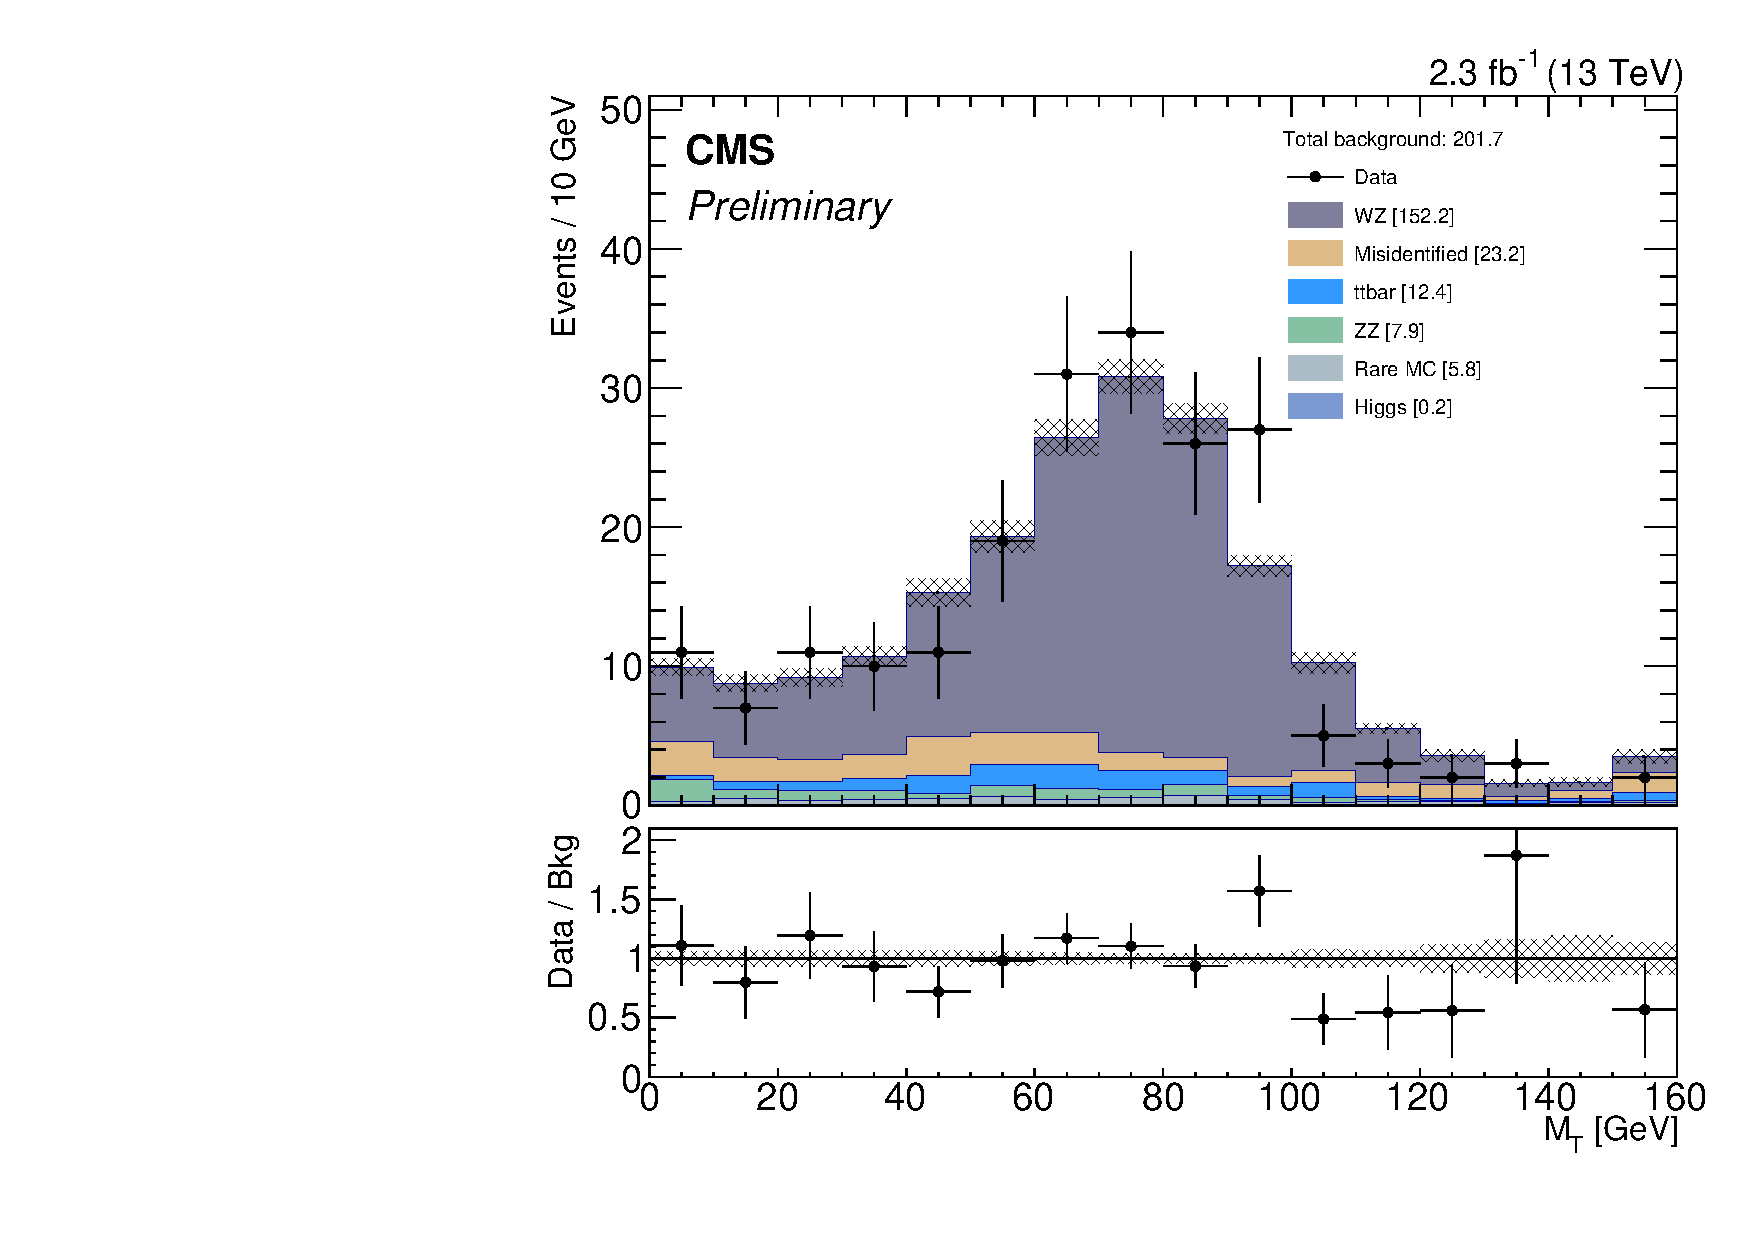
\includegraphics[width=.7\textwidth]{Background/bkg_WZ/WZ_MET50to100_MT}
	\caption{$M_\textrm{T}$ distribution in the \WZ-dominated control region (last bin includes overflow). Uncertainty bands include both statistical and systematic uncertainties, with the exception of the \WZ normalization uncertainty.
	\label{fig:WZ}}
\end{center}
\end{figure}

We validate the prediction in the adjoining $100\,\GeV < \MET < 150\,\GeV$ region and assign a systematic uncertainty of 50\,\% based on the variation of the normalization factor between the normalization region and the validation region.

\section{\texorpdfstring{\ttbar}{TTbar} Background}
\label{sec:bkg_tt}

The \ttbar process contributes about 21\,\% to the total background in our search. We rely on MC to model the process-specific kinematic properties. To that effect, we first verify that the simulation works well in dilepton events, and then correct the MC misidentification rate to match the one in data.

The \ttbar control region is defined by exactly 2 opposite-sign opposite-flavor leptons ($e^\pm \mu^\mp$), at least 1 b-tagged jet above 30\,\GeV, and $\ST > 300\,\GeV$, where \ST is the scalar sum of the lepton transverse momenta, the transverse momenta of jets with $\pt \geq 30\,\GeV$ and $|\eta| \leq 2.4$, and \MET. We use this region to normalize the background prediction. The \MET and \ST distributions are shown in Fig.~\ref{fig:tt2}.

\begin{figure}
\begin{center}
	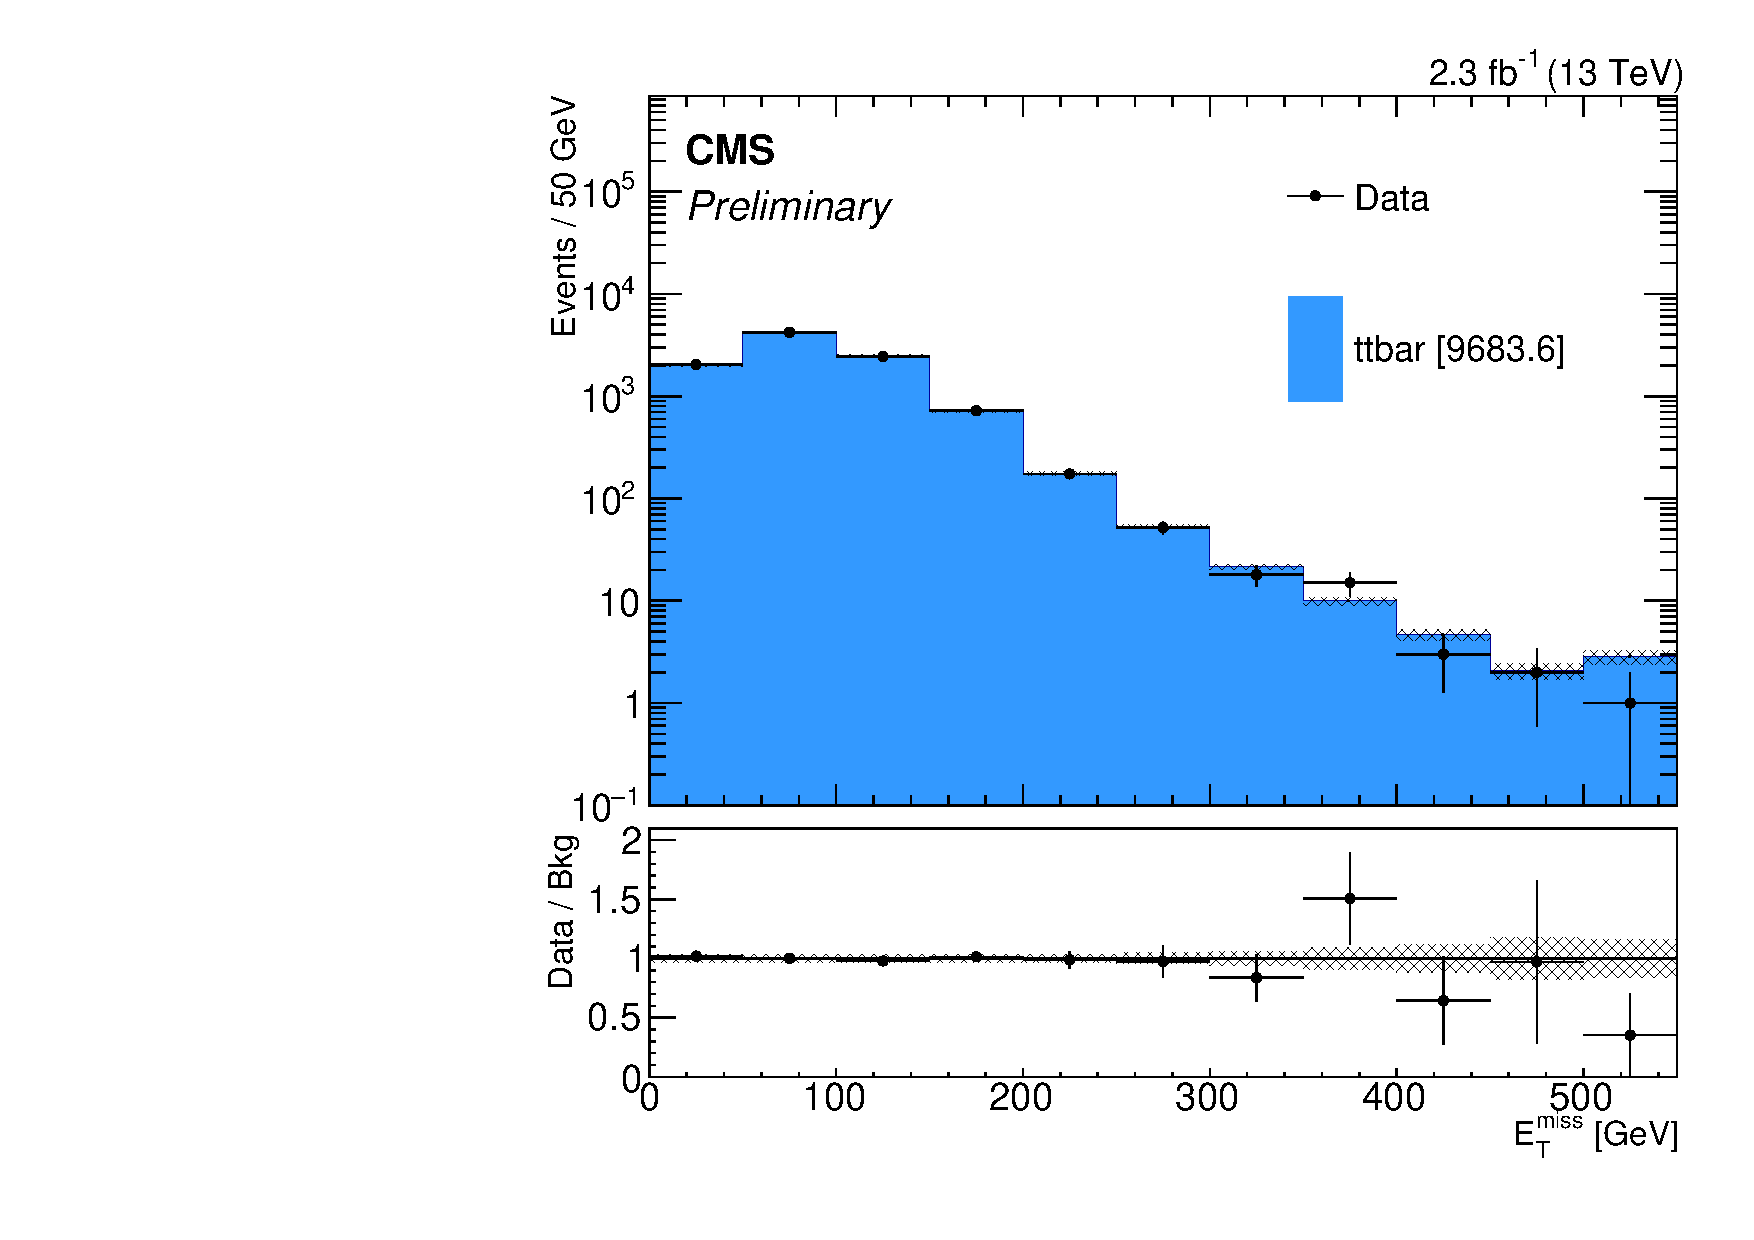
\includegraphics[width=.7\textwidth]{Background/bkg_tt/ttbar_MET_STgt300_afterWeights}
	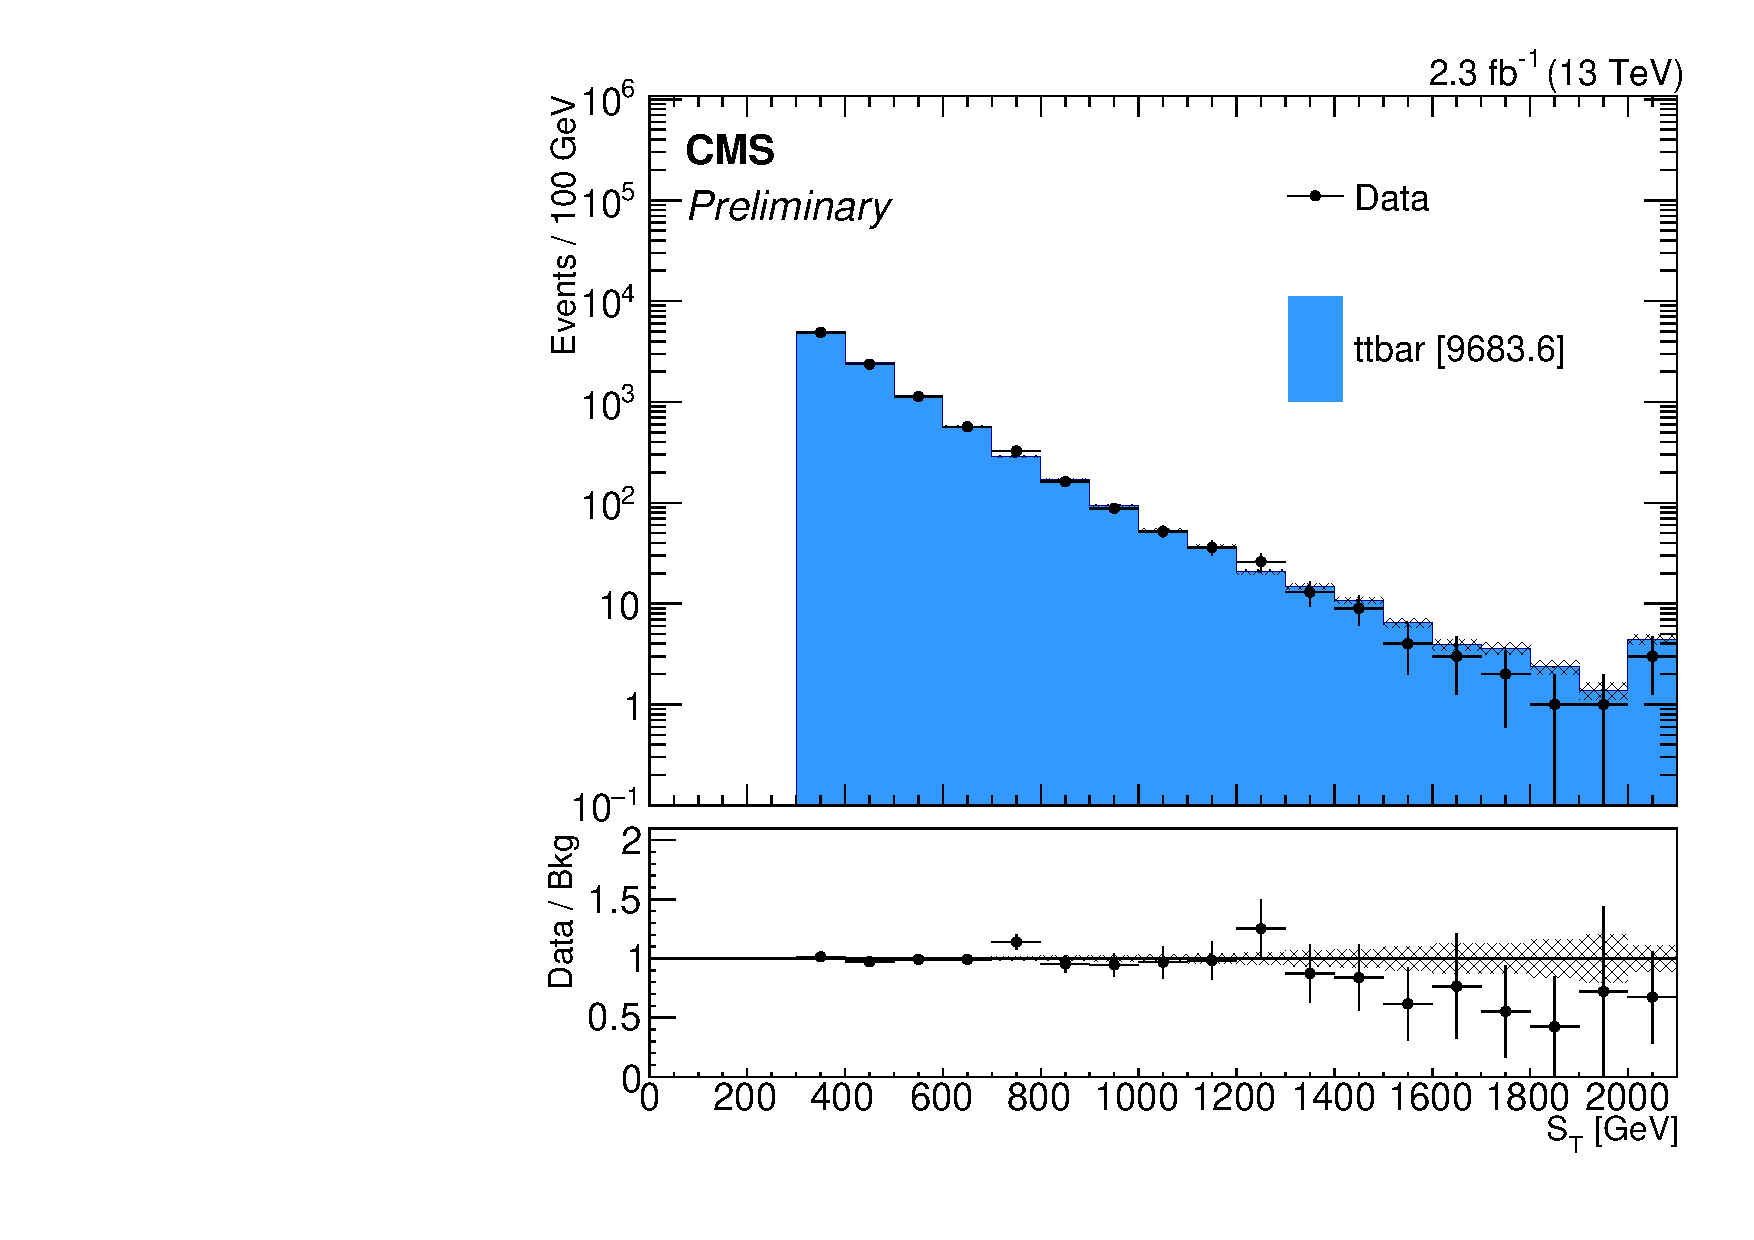
\includegraphics[width=.7\textwidth]{Background/bkg_tt/ttbar_ST_STgt300_afterWeights}
	\caption{\MET (top), and \ST (bottom) distributions in \ttbar-dominated control region (last bin includes overflow). Uncertainties are statistical only.
	\label{fig:tt2}}
\end{center}
\end{figure}

Having established the validity of kinematic aspects of the \ttbar simulation using the dilepton (prompt) sample, we verify that also the rate at which the \ttbar MC produces trilepton events is in agreement with that rate in data. To this end, we measure the lepton misidentification rate in a sample dominated by semi-leptonic \ttbar decays. This sample is selected by requiring one tight muon with $\pt > 30\,\GeV$, 2 jets (from the other top quark), one additional b-tagged jet, and a non-prompt lepton which is most likely misidentified.

We find the misidentification rate in data to be $1.5 \pm 0.5\stat$ times the one found in the \ttbar simulation. This indicates that the number of events with misidentified leptons is underpredicted in the \ttbar simulation. We thus use this ratio to correct the number of predicted trilepton events and apply a systematic uncertainty of 50\,\%.

\section{\texorpdfstring{\Z}{Z} + fake Background}
\label{sec:bkg_fakeLight}

The \Z + fake process contributes about 17\,\% of the total background. Since the misidentified leptons are not modeled with sufficient precision by simulation, we employ a data-driven method that uses correlated objects in order to predict the \Z + fake background.


\subsection{Method}
\label{sec:bkg_fakeLight/Method}

To determine the background with fake electrons and muons, we rely on looser objects measured in data that are emitted in a similar way in the decay chain and are therefore expected to be correlated with the fake leptons, and use them as lepton proxies.\footnote{These looser objects are not necessarily leptons as well. For example, a photon that converts into two leptons, one of which has very low \pt, may have kinematics which are very similar to the ones of the other conversion lepton that carries most of the \pt. (Of course, the selection of such objects may be tricky.)} We verify that the kinematic properties of these proxies resemble those of the fake leptons. We then generate a fake sample based on the 2$\ell$+[proxy object] data, treating the proxy objects as leptons (``seed sample''). Further down in the analysis chain, these fake leptons simply appear as regular leptons (\eg when computing invariant masses). Proxy objects that can take multiple roles are considered the appropriate number of times (see below).

The number of 3$\ell$ events in data per 2$\ell$+[proxy object] event in this fake sample is then evaluated (``fake rate''). With the help of the fake rate, we predict the background in the signal regions, by applying it to the corresponding seed sample which requires one less lepton and a proxy object instead. Because the proxy objects appear as leptons, this is simply done by selecting the signal region from the fake sample and multiplying the yield by the fake rate.

To compute the fake rate $\frac{N(3\ell)}{N(2\ell + \textrm{[proxy object])}}$, we subtract contributions from other backgrounds in the numerator and the denominator. This step interacts with the MC background normalizations and thus requires an iterative process to converge. The fake rate then describes the number of fake leptons as a fraction of the number of 2$\ell$+[proxy object] events from all processes that have not been modeled otherwise.

When we apply the fake rate in a signal region, we multiply it by the total number of 2$\ell$+[proxy object] events found in the corresponding seed region in data. However, we use MC to obtain the fake contribution for certain backgrounds.\footnote{This is especially important for \ttbar when a b-tag is not present, since the fake rate is higher in \ttbar events, but there is no obvious way to discern these events from non-\ttbar events in the seed sample.} In these cases, double-counting needs to be mitigated. Therefore, we take the 2$\ell$+[proxy object] component of the background MC sample, apply the same fake rate as for data, and subtract the resulting prediction from the regular data-driven prediction (see \eg Sec.~\ref{sec:bkg_tt} for \ttbar). This is equivalent to keeping the seed sample clean of proxies originating from processes that are modeled otherwise. We therefore verify that the number of tracks be modeled correctly in MC (see Sec.~\ref{sec:bkg_tt/dilepton+track}).

In rare cases due to statistical fluctuations, the subtraction might yield a (small) negative number. If that happens, we replace it by zero, to make sure that the background prediction behaves physically reasonably.\footnote{Another option would be to subtract the MC-fake-seed-driven background from the regular \ttbar MC prediction (again with a lower bound at 0). However, 8\,\TeV cross-checks have shown that this leads to less accurate results.}

%We also study to what extent the fake rate depends on other properties of the event (for example the jet composition and spectra), and parameterize the fake rate as necessary. The freedom that we find in determining these parameterizations and kinematic weights is used to assess the systematic uncertainty of the background estimate.

\subsection{Fake Leptons from Asymmetric Internal Photon Conversions (AIC)}
\label{sec:bkg_fakeLight/photons}
We look at the number of events that have 3 light leptons (no $\tau_\textrm{had}$) including an OSSF pair below \Z (\ie $m_{\ell\ell} < 81\,\GeV$), no b-tags, $\HT < 200\,\GeV$, and $\MET < 50\,\GeV$. This is essentially the \Z peak region, except that the dilepton invariant mass is not large enough to fall on the \Z peak, and a third lepton is present.

This region primarily contains events from $\Z \to \ell\ell$ where one of the final state leptons radiates an off-shell photon which decays, or\hairspace---\hairspace{}equivalently\hairspace---\hairspace{}internally converts, asymmetrically to two additional leptons, one of which carries very low \pt and is not reconstructed as an independent object in the detector. The process of emission of an off-shell photon through asymmetric internal conversion then yields a single reconstructed lepton in the detector \cite{Gray:2011us}. Since the \pt of the lost lepton is low, the leading three leptons nearly reconstruct the invariant mass of the Z peak. The internal conversion process has an infrared singularity, so the distribution of off-shell photon masses is peaked at very low values. The resulting kinematic distribution in this region of phase space is then very similar to the emission of a real on-shell photon. 

We may therefore form a seed sample with photons as proxies for fake leptons coming from asymmetric internal conversion. All combinations are taken into account, \ie dilepton events with a photon enter the fake sample as four event types (two possible flavors, two possible charges). The photons are required to be within $0.30 \leq \Delta R \leq 0.60$ from another light lepton. This is the characteristic distance for radiated photons of the type considered, as can be seen from Fig.~\ref{fig:fakeLight_AIC_DR}.

\begin{figure}
\begin{center}
	\begin{subfigure}[b]{.7\textwidth}
		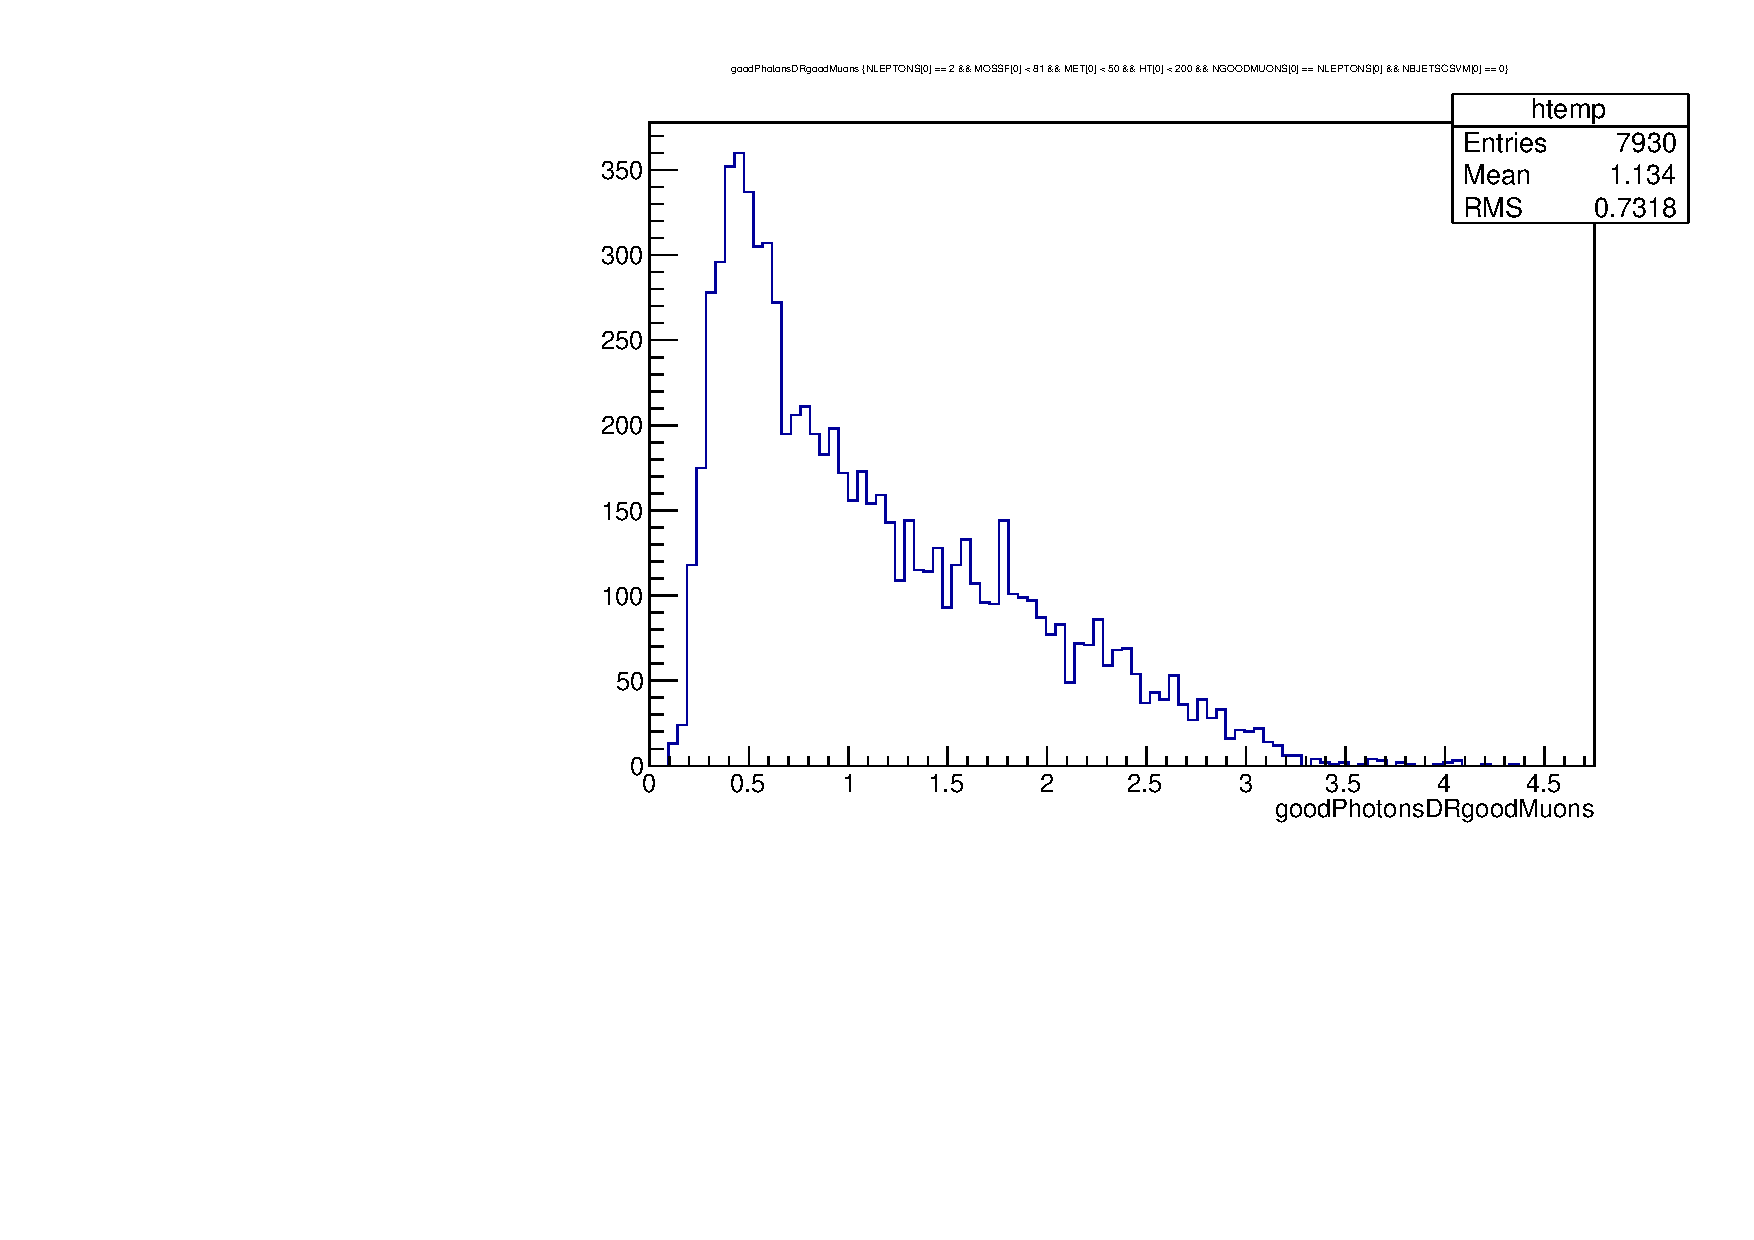
\includegraphics[width=\textwidth]{Background/bkg_fakeLight/goodPhotonsDRgoodMuons_AIC}
		\caption{AIC control region}
	\end{subfigure}
	\begin{subfigure}[b]{.7\textwidth}
		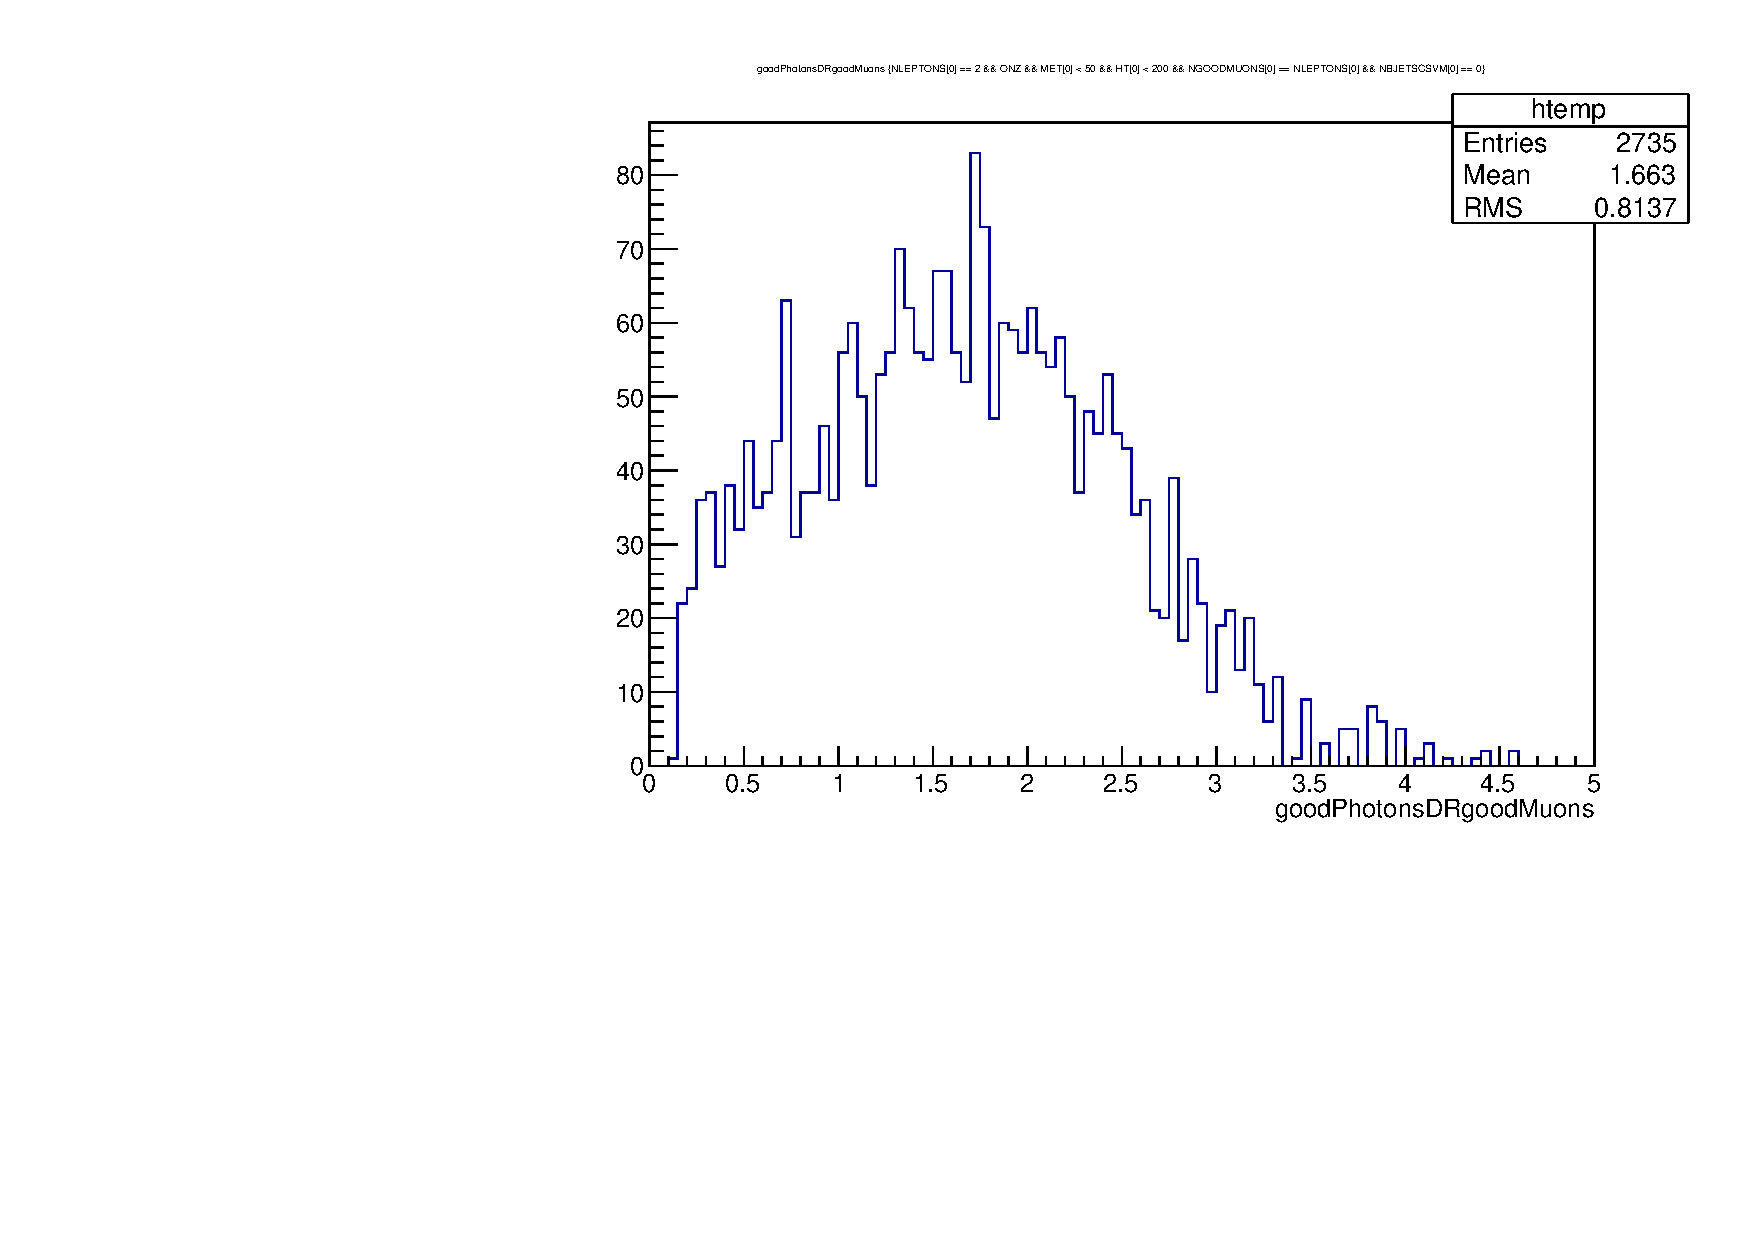
\includegraphics[width=\textwidth]{Background/bkg_fakeLight/goodPhotonsDRgoodMuons_ONZ}
		\caption{dilepton region on-\Z}
	\end{subfigure}
	\caption{$\Delta R$ distributions between photon and muon
	\label{fig:fakeLight_AIC_DR}}
\end{center}
\end{figure}

Looking in the seed sample, we find that the $2\ell+\gamma$ mass indeed reproduces the \Z peak, as shown in Fig.~\ref{fig:fakeLight_AIC_MLEPTONS}. For photons faking muons, we find better shape agreement if we apply a loss factor of 0.8 to the photon \pt when creating the fake trilepton sample, attributing an average of 20\,\% of the \pt to the lost lepton. Outside the trilepton \Z window, it is necessary to increase the fake rate by 1.8 to achieve agreement.

\begin{figure}
\begin{center}
	\begin{subfigure}[b]{.7\textwidth}
		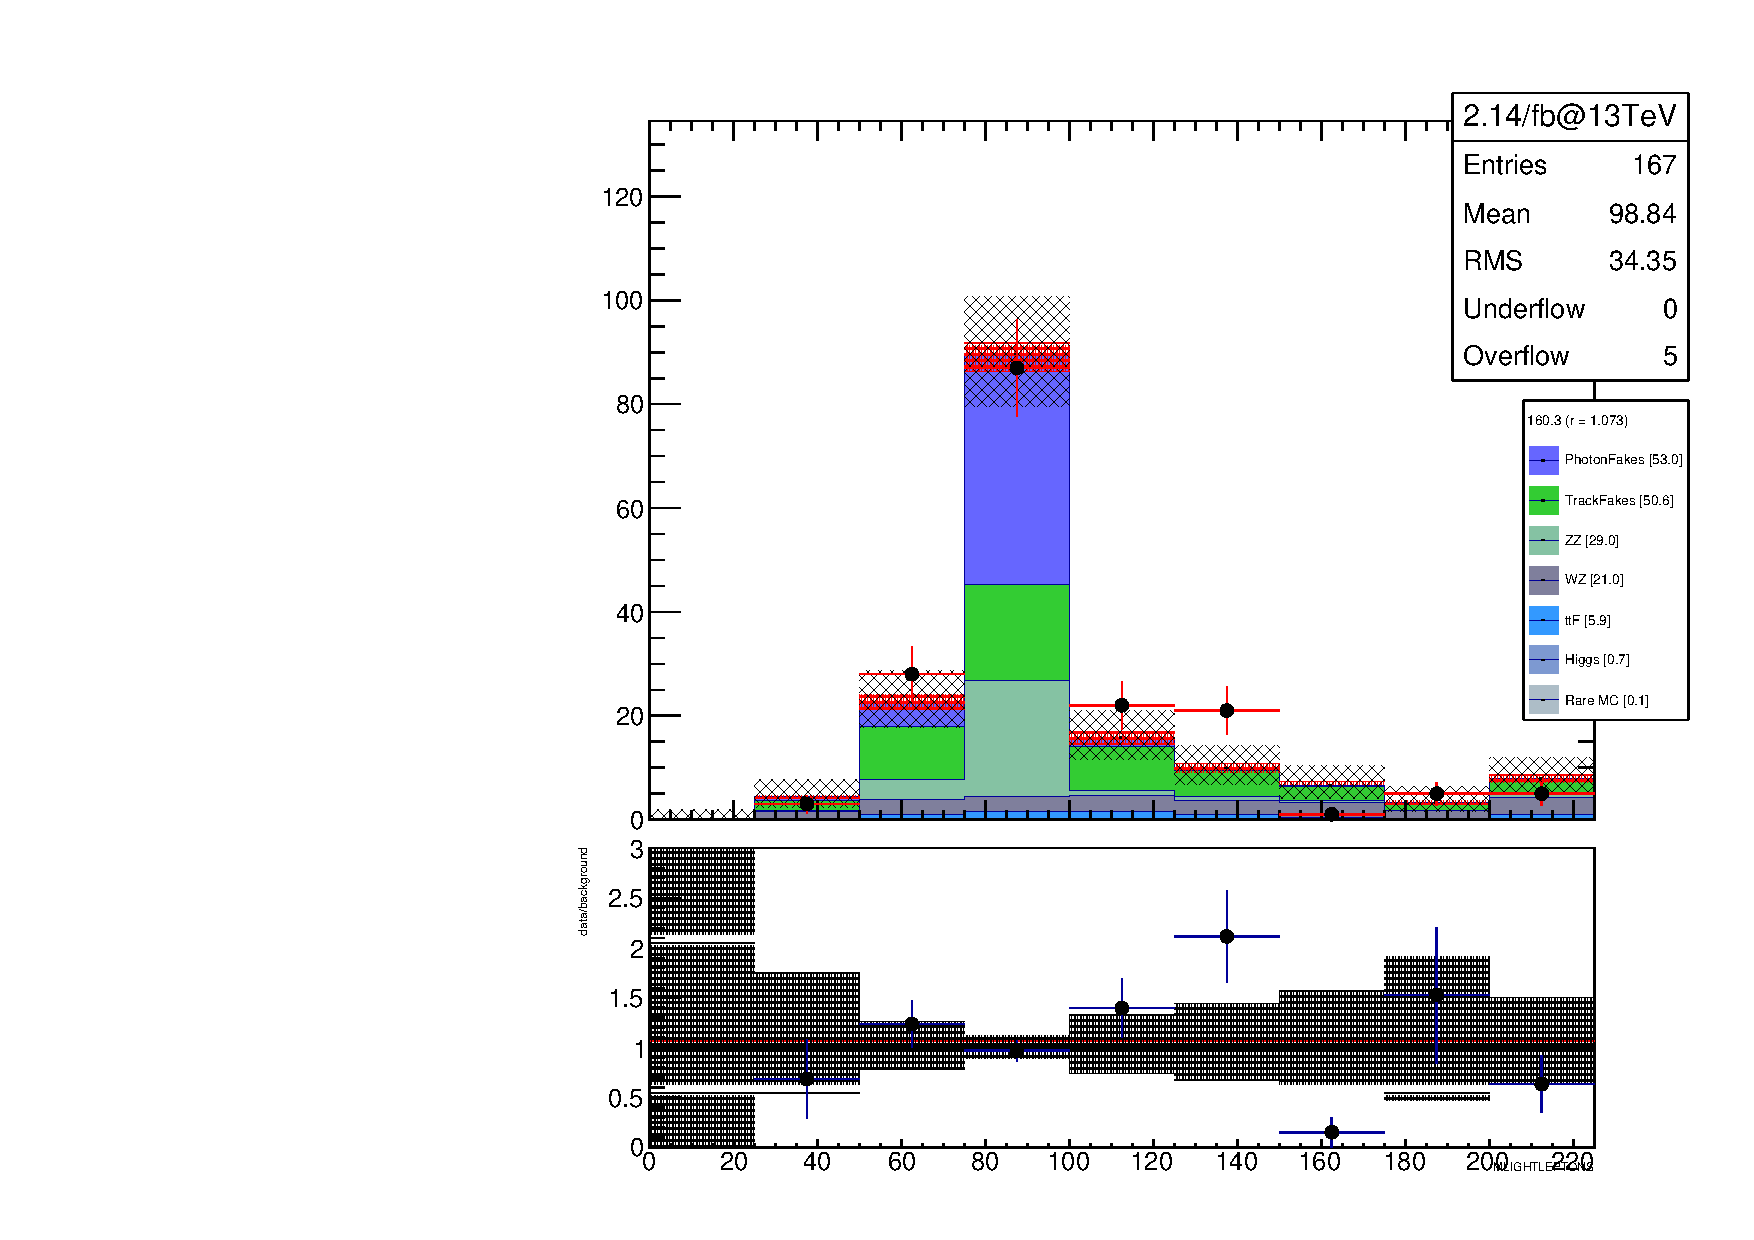
\includegraphics[width=\textwidth]{Background/bkg_fakeLight/AIC_MLIGHTLEPTONS_muFake}
		\caption{fake muon}
	\end{subfigure}
	\begin{subfigure}[b]{.7\textwidth}
		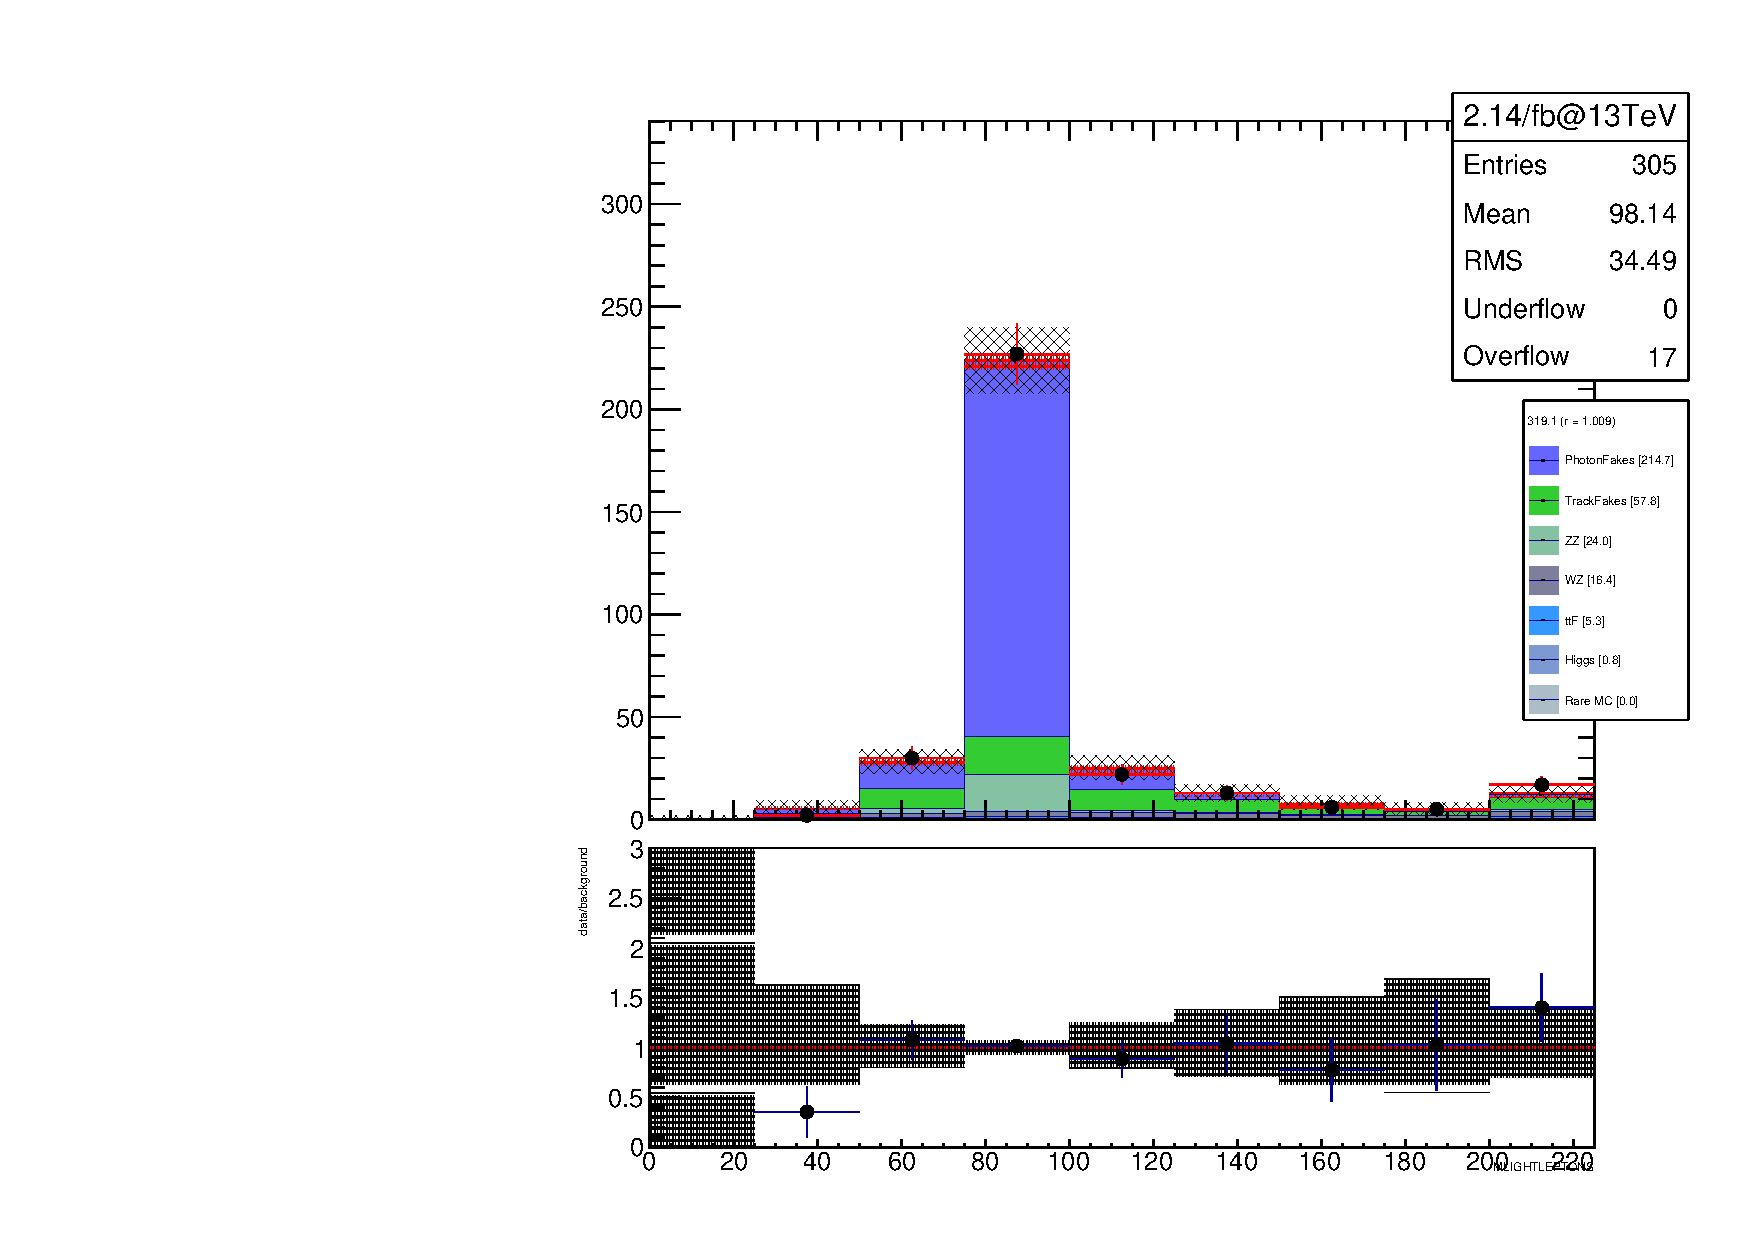
\includegraphics[width=\textwidth]{Background/bkg_fakeLight/AIC_MLIGHTLEPTONS_elFake}
		\caption{fake electron}
	\end{subfigure}
	\caption{$m_{3\ell}$ distribution in AIC-dominated control region.
	\label{fig:fakeLight_AIC_MLEPTONS}}
\end{center}
\end{figure}

After these corrections, we find that the photon fake rates are
\begin{itemize}
	\item muons: 1.60\,\% ($ee$ environment), 1.05\,\% ($\mu\mu$ environment),
	\item electrons: 3.5\,\% ($ee$ environment), 4.5\,\% ($\mu\mu$ environment).
\end{itemize}

We apply a 52\,\% systematic uncertainty on the total photon-based background estimate. This is because the photon fake rate depends on the environment flavor within this range.


\subsection{Fake Leptons from Jets}
In order to determine the background with misidentified electrons and muons from jets, we use isolated tracks a proxies. The isolation criteria that we require these tracks to satisfy are identical to our muon isolation criteria (see Sec.~\ref{sec:Selection/Object}). We produce a track-based fake 3$\ell$ background seed sample by reassigning isolated tracks to the lepton collections, so that the sample has one less lepton than the signal regions and an isolated track instead. All combinations are taken into account, \ie tracks are used to create both a fake-$e$ and a fake-$\mu$ event.\footnote{Multiple fakes in an event are not considered (neither of same proxy type (\eg two tracks) nor of different type). Hybrid fakes (one from a track, one from a photon) are currently not supported for technical reasons; same-type fakes however turned out to cause problems with the \ttbar MC subtraction. Given the smallness of the fake rates ($O(10^{-2})$), the contribution from multiple fakes is negligible anyways.} The fake background can then be estimated by applying the fake rate after requiring the signal region selection in this seed sample.

The fake rate $\frac{N(3\ell)}{N(2\ell + \textrm{track)}}$ is determined using events with 3 electrons or muons including an OSSF pair on-\Z and $\MET < 50\,\GeV$. This is the prominent \Z peak region with an additional lepton. As we subtract contributions from other backgrounds in the numerator and the denominator, this misidentification rate describes the number of misidentified leptons as a fraction of the number of 2$\ell$ + track events from all processes that are not modeled otherwise.

To achieve the best possible modeling, we make sure that the kinematic properties of the isolated tracks in this region resemble those of the misidentified leptons by applying weights to the track-based background in bins of the the lowest \pt lepton (proxy) which is generally the fake (Fig.~\ref{fig:fakeLight_Z_MINleptonPT}). Appendix~\ref{app:MOSSFlepton,track} contains additional plots supporting the suitability of tracks as lepton proxies. We then measure the number of 3$\ell$ events in data per 2$\ell$ + track event (fake rate), as a function of the flavor of both the fake lepton and of the \Z decay products and find:
\begin{itemize}
	\item muons: $(1.49 \pm 0.21)\,\%$ ($ee$ environment), $(1.49 \pm 0.17)\,\%$ ($\mu\mu$ environment),
	\item electrons: $(1.37 \pm 0.22)\,\%$ ($ee$ environment), $(1.75 \pm 0.19)\,\%$ ($\mu\mu$ environment).
\end{itemize}
Based on this, we use the electron and muon fake rates $(1.59 \pm 0.15\stat)\,\%$ and $(1.49 \pm 0.13\stat)\,\%$, respectively. We apply a systematic uncertainty of 14\,\% to cover the variation of observed misidentification rates as a function of the flavor of the remaining prompt lepton pair in the event.

To apply the misidentification rate in a signal region, we multiply it by the total number of events found in the corresponding 2$\ell$ + track region in data. However, since we use MC to obtain the misidentified contribution for the \ttbar background, we need to correct for double-counting. We thus subtract the contribution from 2$\ell$ + track events as predicted by the \ttbar MC from the data. To show that the subtraction is valid, we verify that the $n_\textrm{tracks}$ distribution in the \ttbar MC sample matches the one in data, so that we can trust the fake rate method used in data is applicable for the \ttbar MC subtraction (see Sec.~\ref{sec:bkg_tt}).

\begin{figure}
\begin{center}
	\begin{subfigure}[b]{.7\textwidth}
		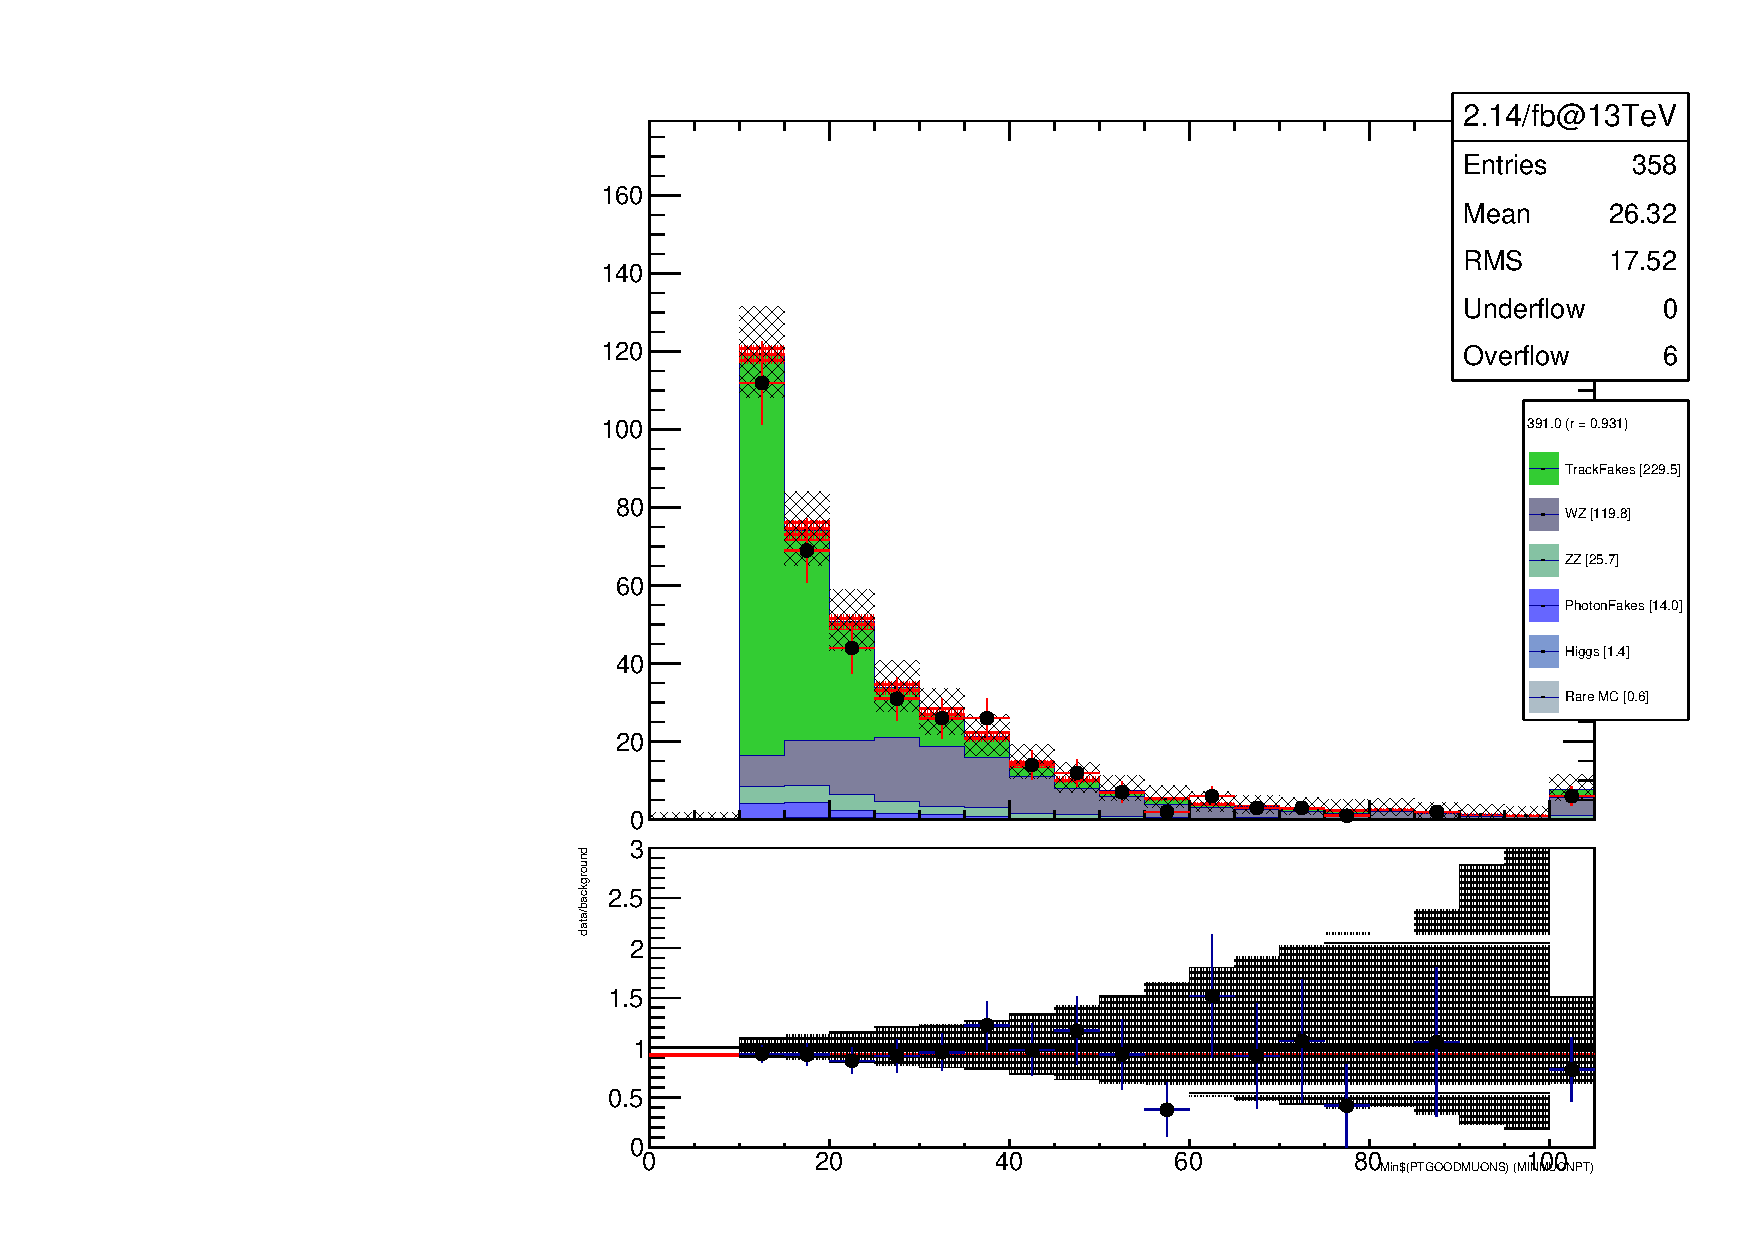
\includegraphics[width=\textwidth]{Background/bkg_fakeLight/Z_muFake_MINMUONPT}
		\caption{fake muon}
	\end{subfigure}
	\begin{subfigure}[b]{.7\textwidth}
		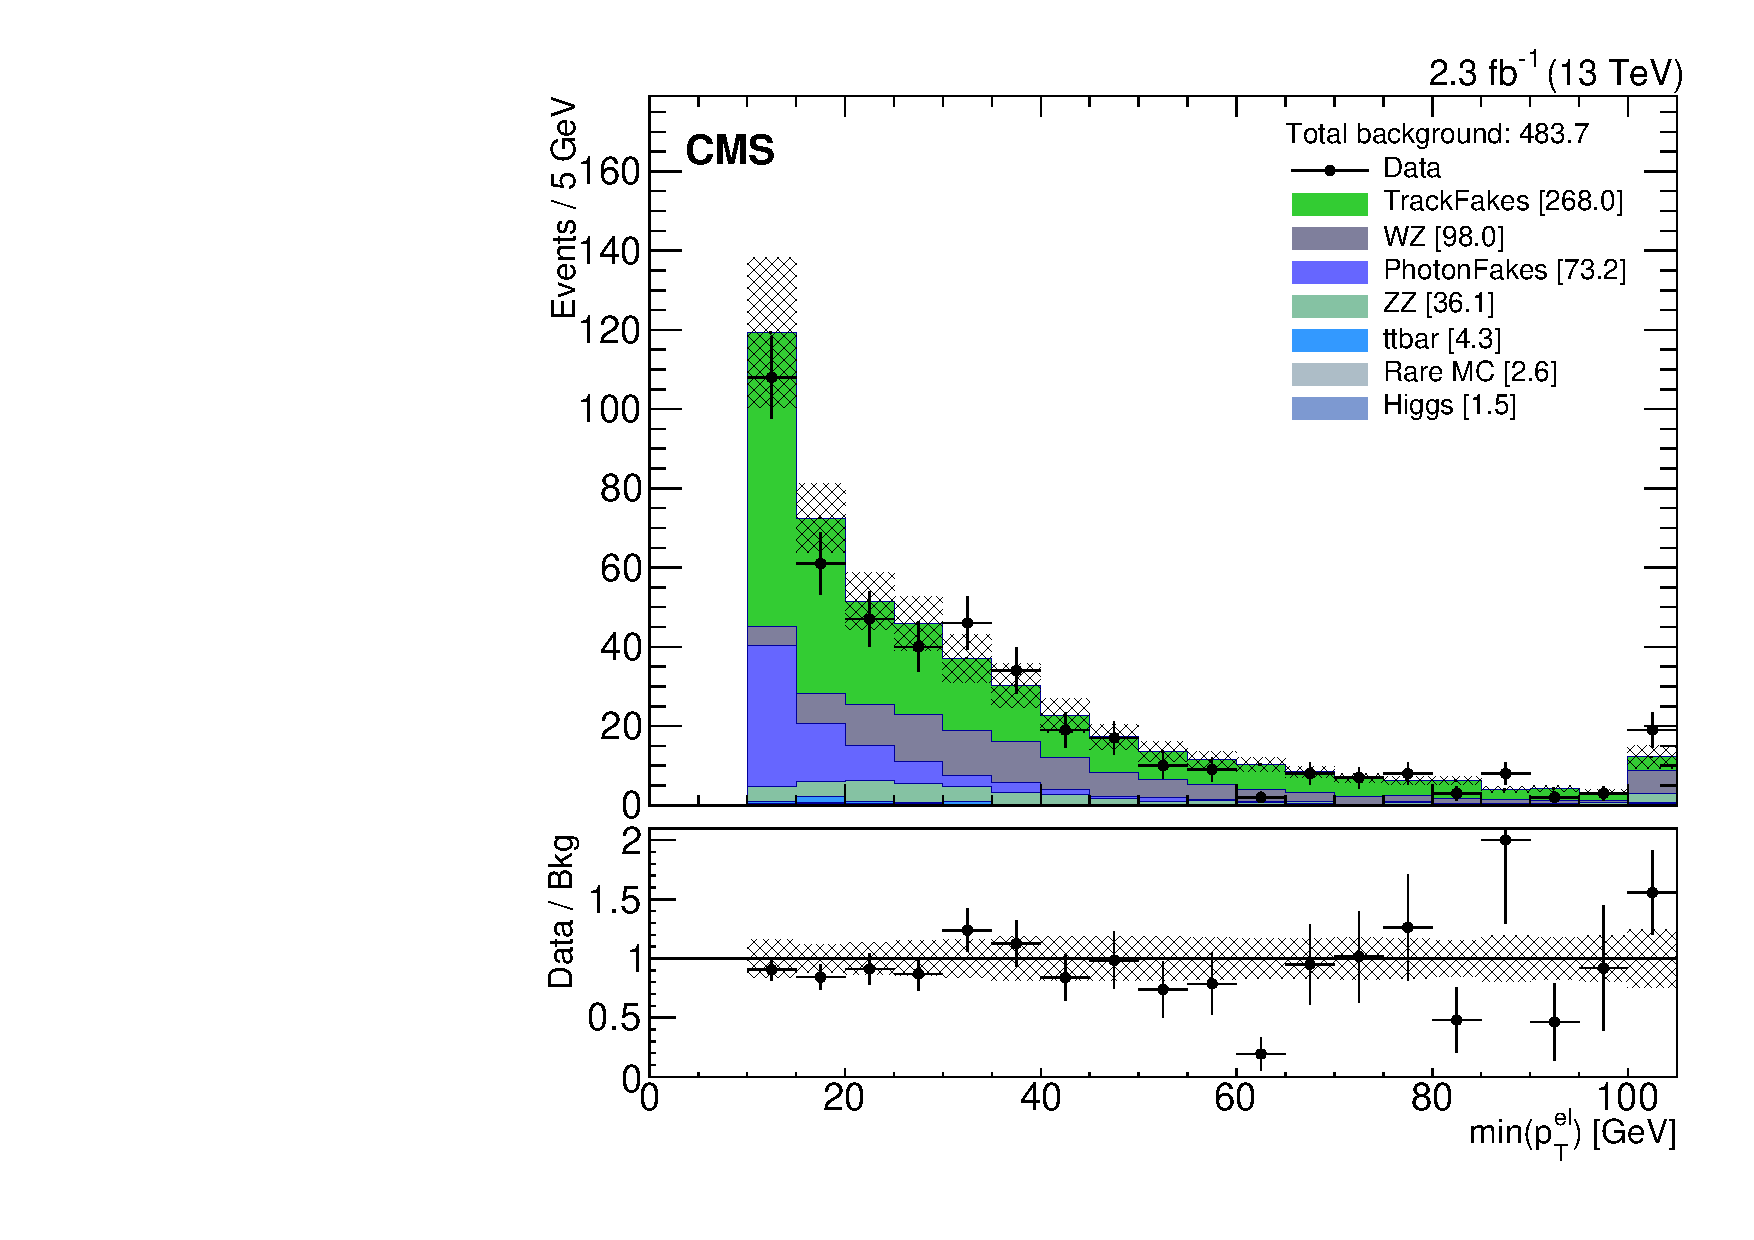
\includegraphics[width=\textwidth]{Background/bkg_fakeLight/Z_elFake_MINELECTRONPT}
		\caption{fake electron}
	\end{subfigure}
	\caption{\pt distributions of the lowest \pt lepton.
	\label{fig:fakeLight_Z_MINleptonPT}}
\end{center}
\end{figure}

Fig.~\ref{fig:fakeLight_Z_MOSSF} shows the mass distribution of the ``best'' OS dilepton pair across its full range in the trilepton control region, both with and without an AIC veto (for off-\Z events whose 3$\ell$ invariant mass is on \Z); Fig.~\ref{fig:fakeLight_Z_MOSSF_byFlavor} distinguishes by flavors. In case of ambiguity, the ``best'' OS dilepton pair is the one whose invariant mass is closest to the \Z mass, with the additional condition that pairs above the \Z window are not considered if there is a pair below the \Z window (thus shifting events from high-\Z to low-\Z, for a more separative background categorization, see Sec.~\ref{sec:Strategy/general}).

\begin{figure}
\begin{center}
	\begin{subfigure}[t]{.7\textwidth}
		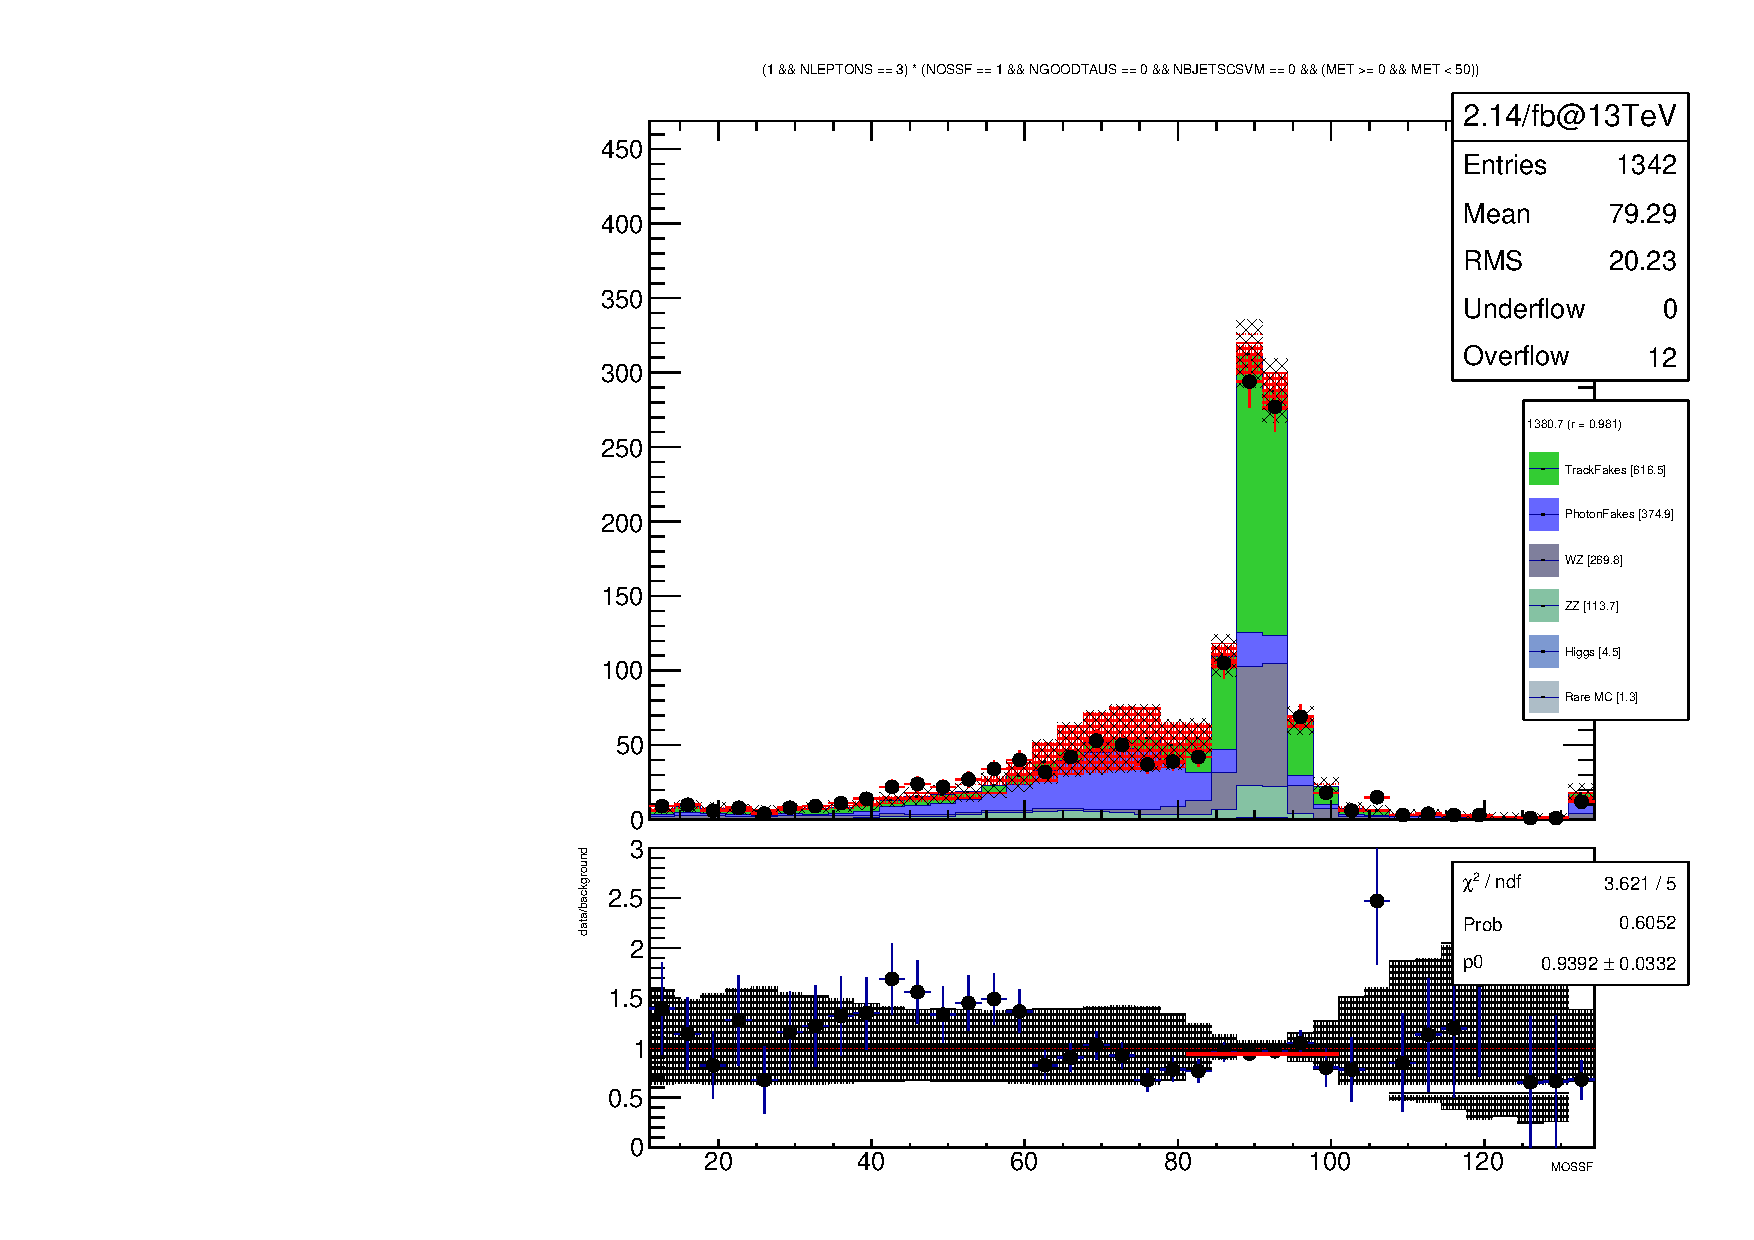
\includegraphics[width=\textwidth]{Background/bkg_fakeLight/Z_MOSSF}
		\caption{including events with $m_{\ell\ell\ell}$ on-\Z}
	\end{subfigure}
	\begin{subfigure}[t]{.7\textwidth}
		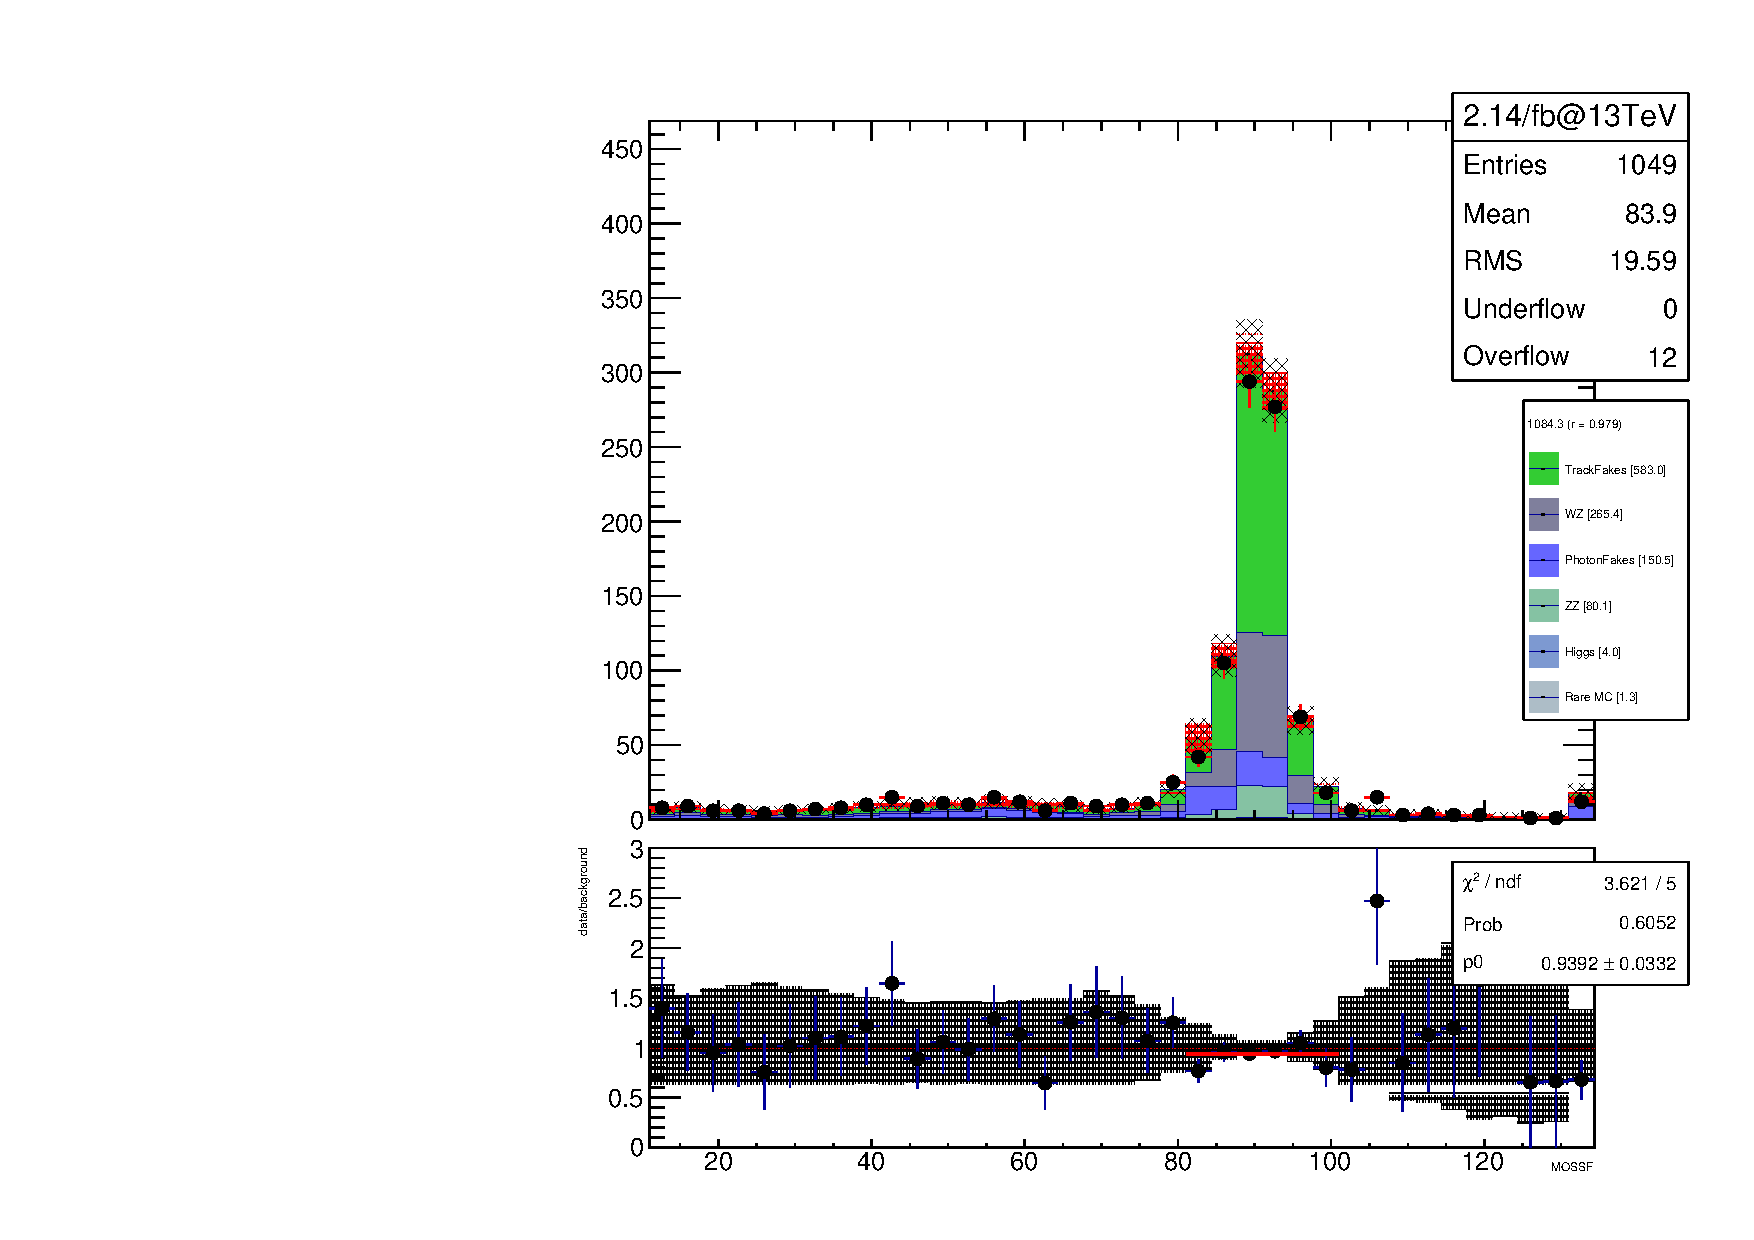
\includegraphics[width=\textwidth]{Background/bkg_fakeLight/Z_noAIC_MOSSF}
		\caption{events with $m_{\ell\ell\ell}$ on-\Z removed from the dilepton-off-\Z regions}
	\end{subfigure}
	\caption{$m_{\ell\ell}$ distribution in the dilepton + fake region.
	\label{fig:fakeLight_Z_MOSSF}}
\end{center}
\end{figure}

\begin{figure}
\begin{center}
	\begin{subfigure}[b]{.5\textwidth}
		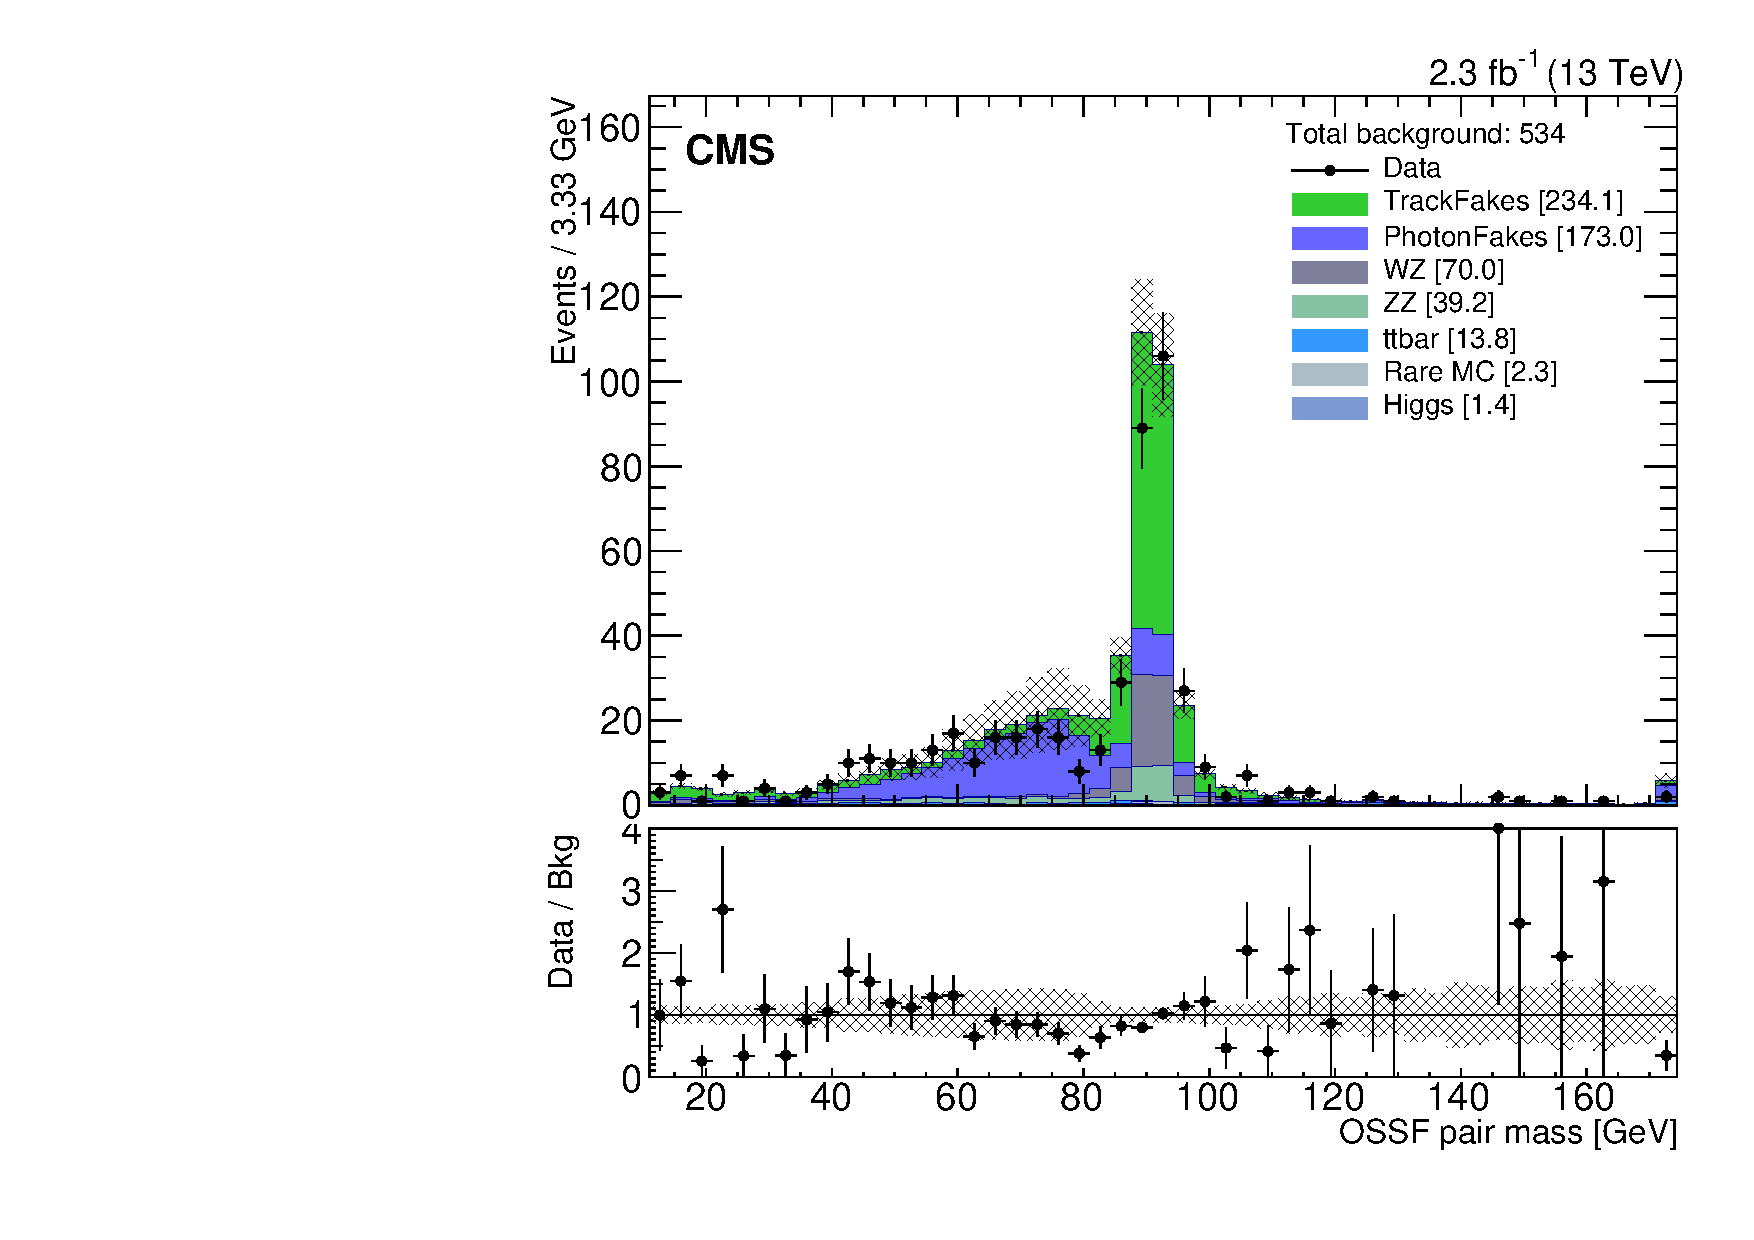
\includegraphics[width=\textwidth]{Background/bkg_fakeLight/Z_1el2mu_MOSSF}
		\caption{$e$ fake, $\Z \to \mu\mu$}
	\end{subfigure}%
	\begin{subfigure}[b]{.5\textwidth}
		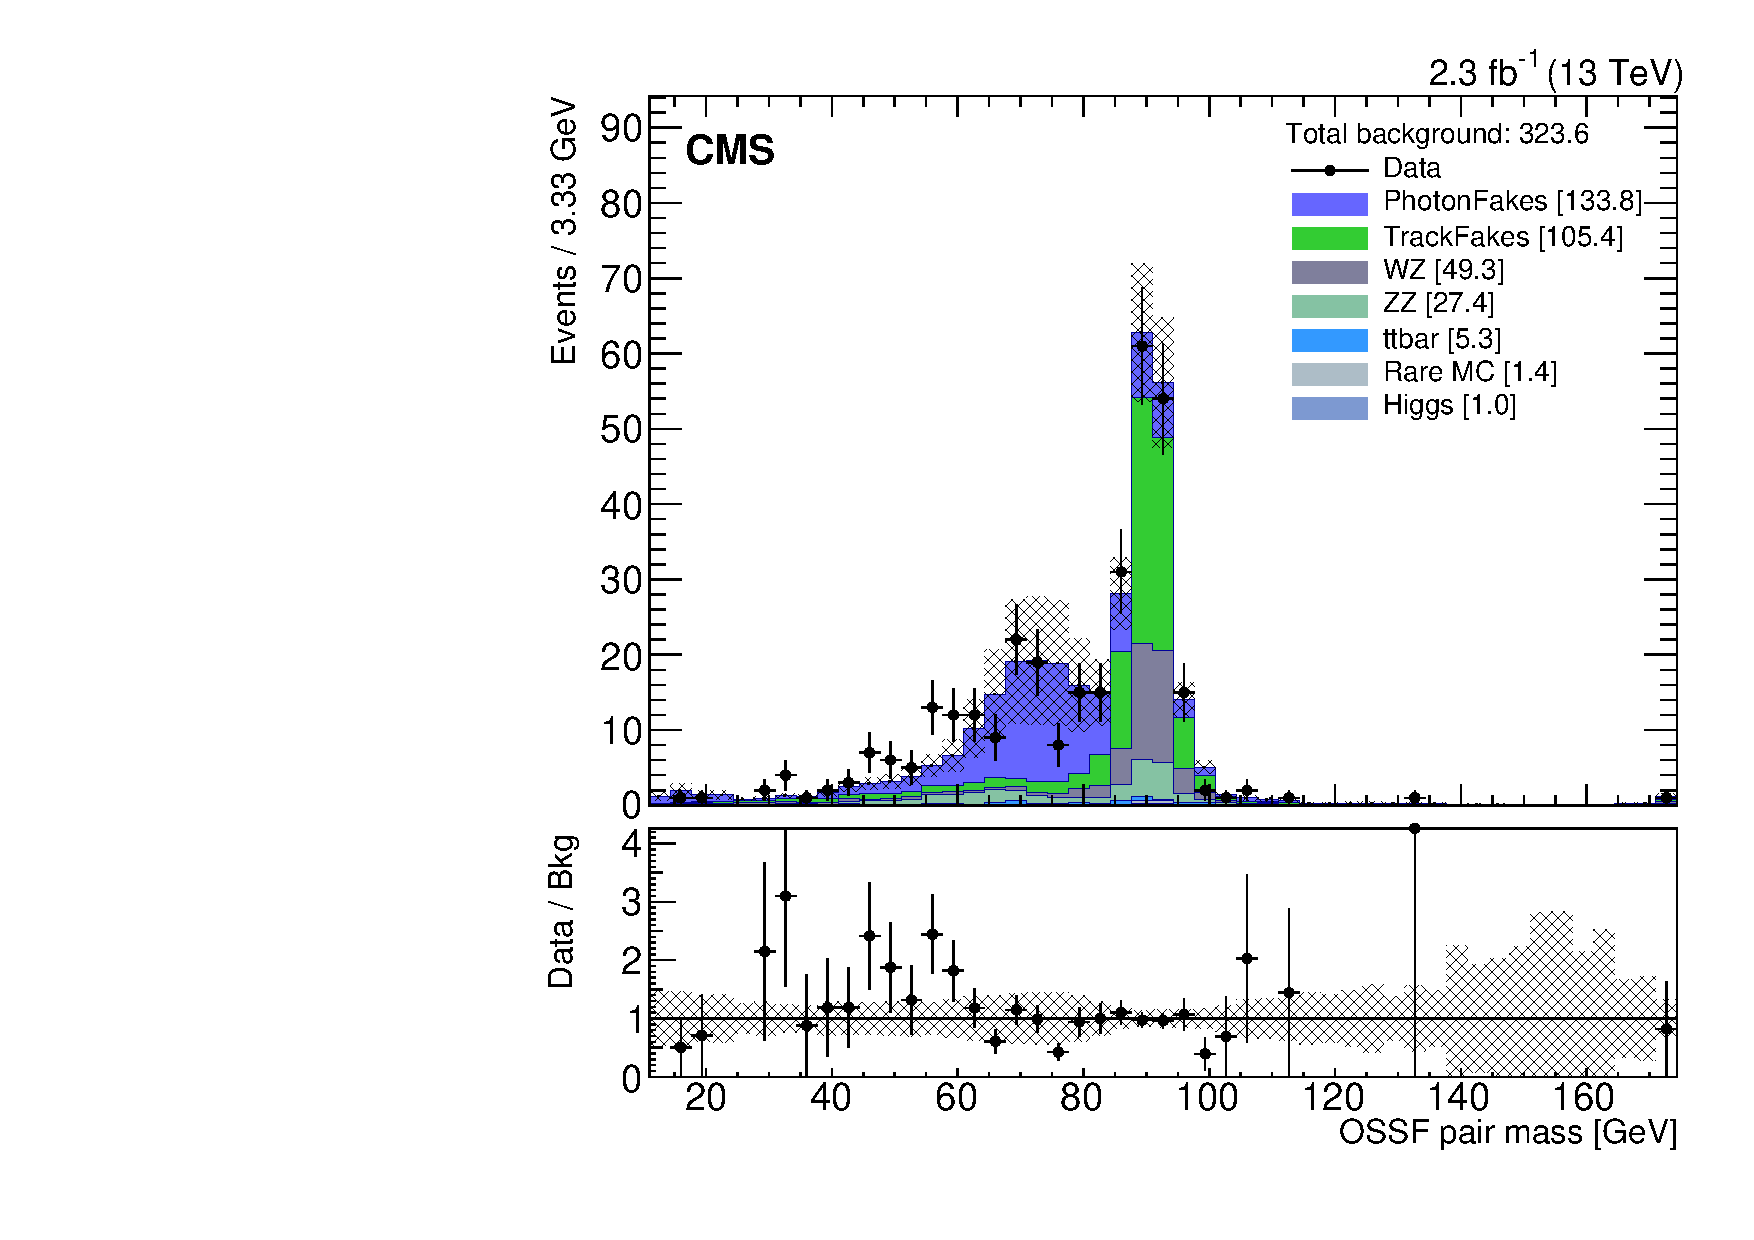
\includegraphics[width=\textwidth]{Background/bkg_fakeLight/Z_3el_MOSSF}
		\caption{$e$ fake, $\Z \to e e$}
	\end{subfigure}
	\begin{subfigure}[b]{.5\textwidth}
		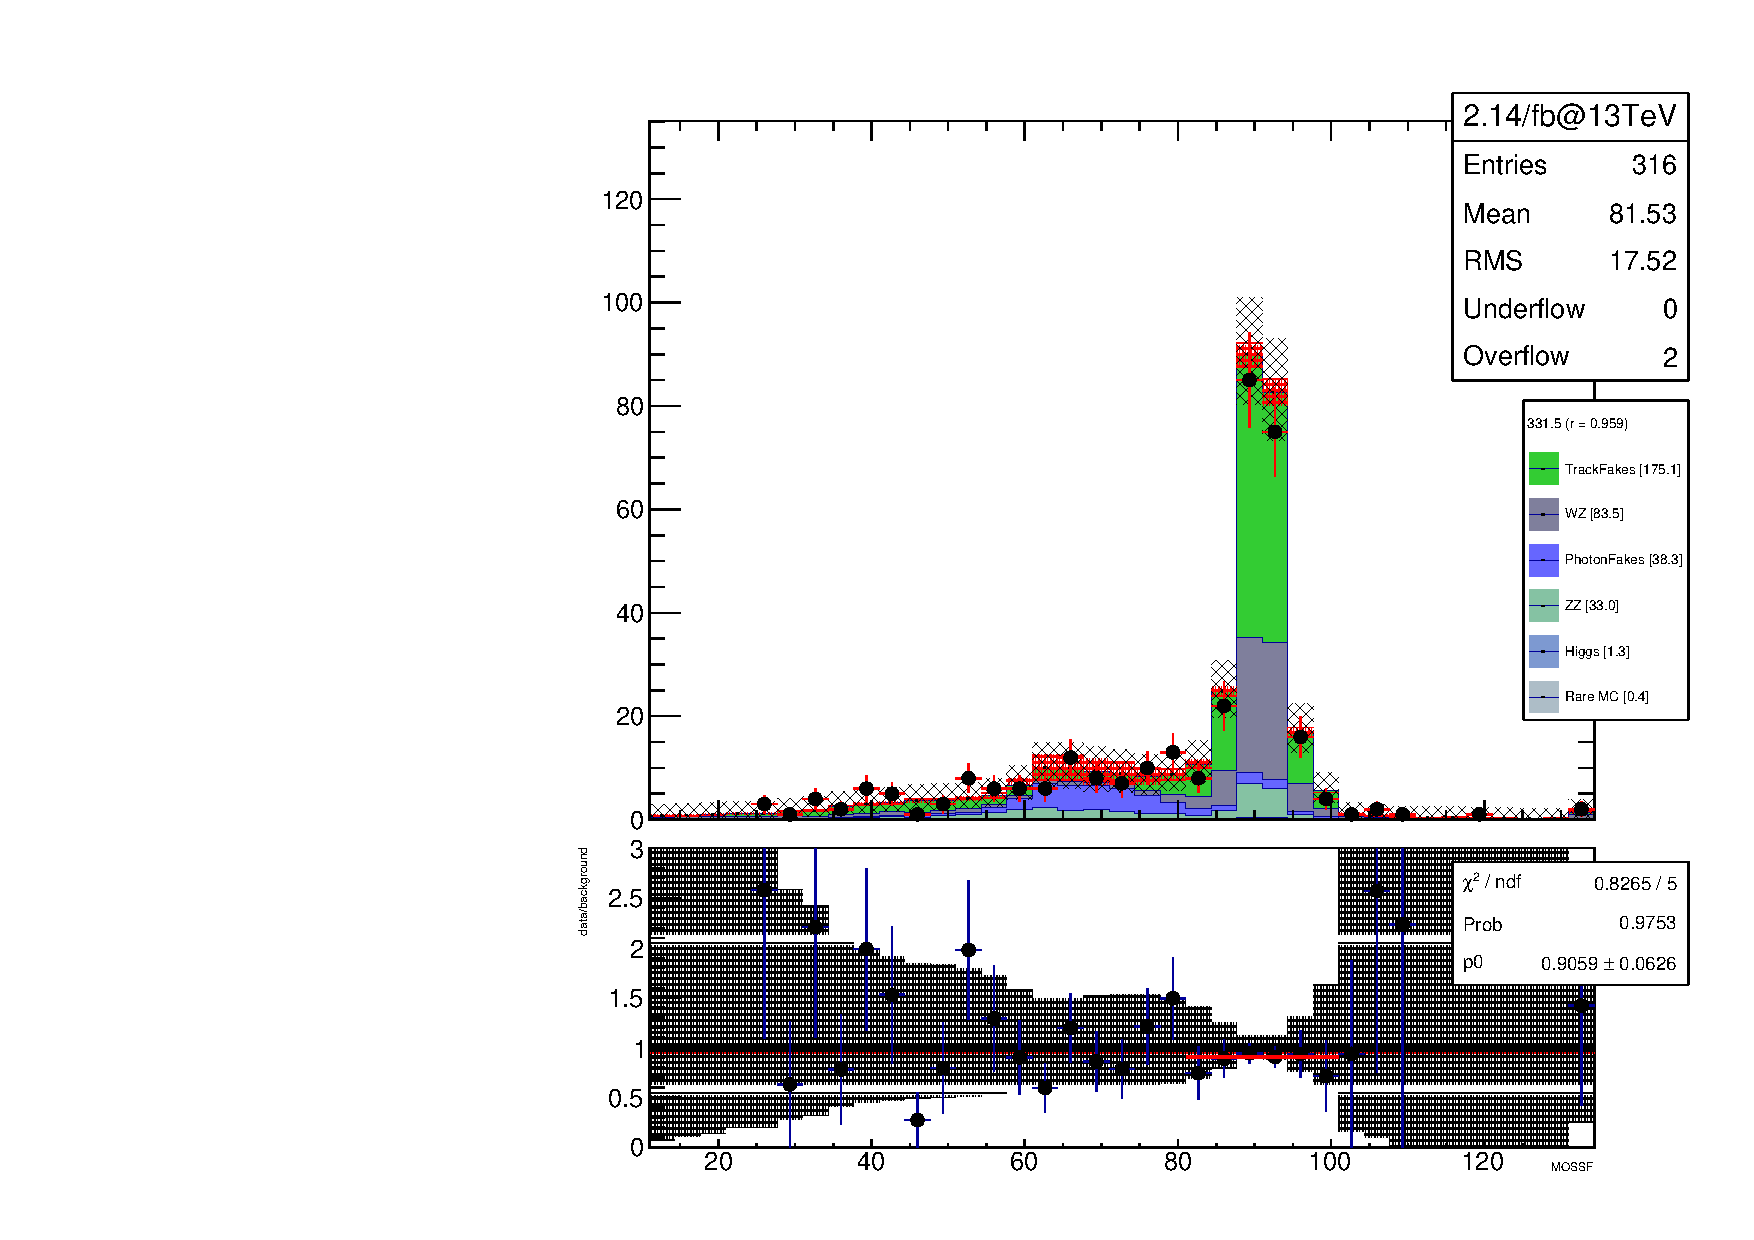
\includegraphics[width=\textwidth]{Background/bkg_fakeLight/Z_3mu_MOSSF}
		\caption{$\mu$ fake, $\Z \to \mu\mu$}
	\end{subfigure}%
	\begin{subfigure}[b]{.5\textwidth}
		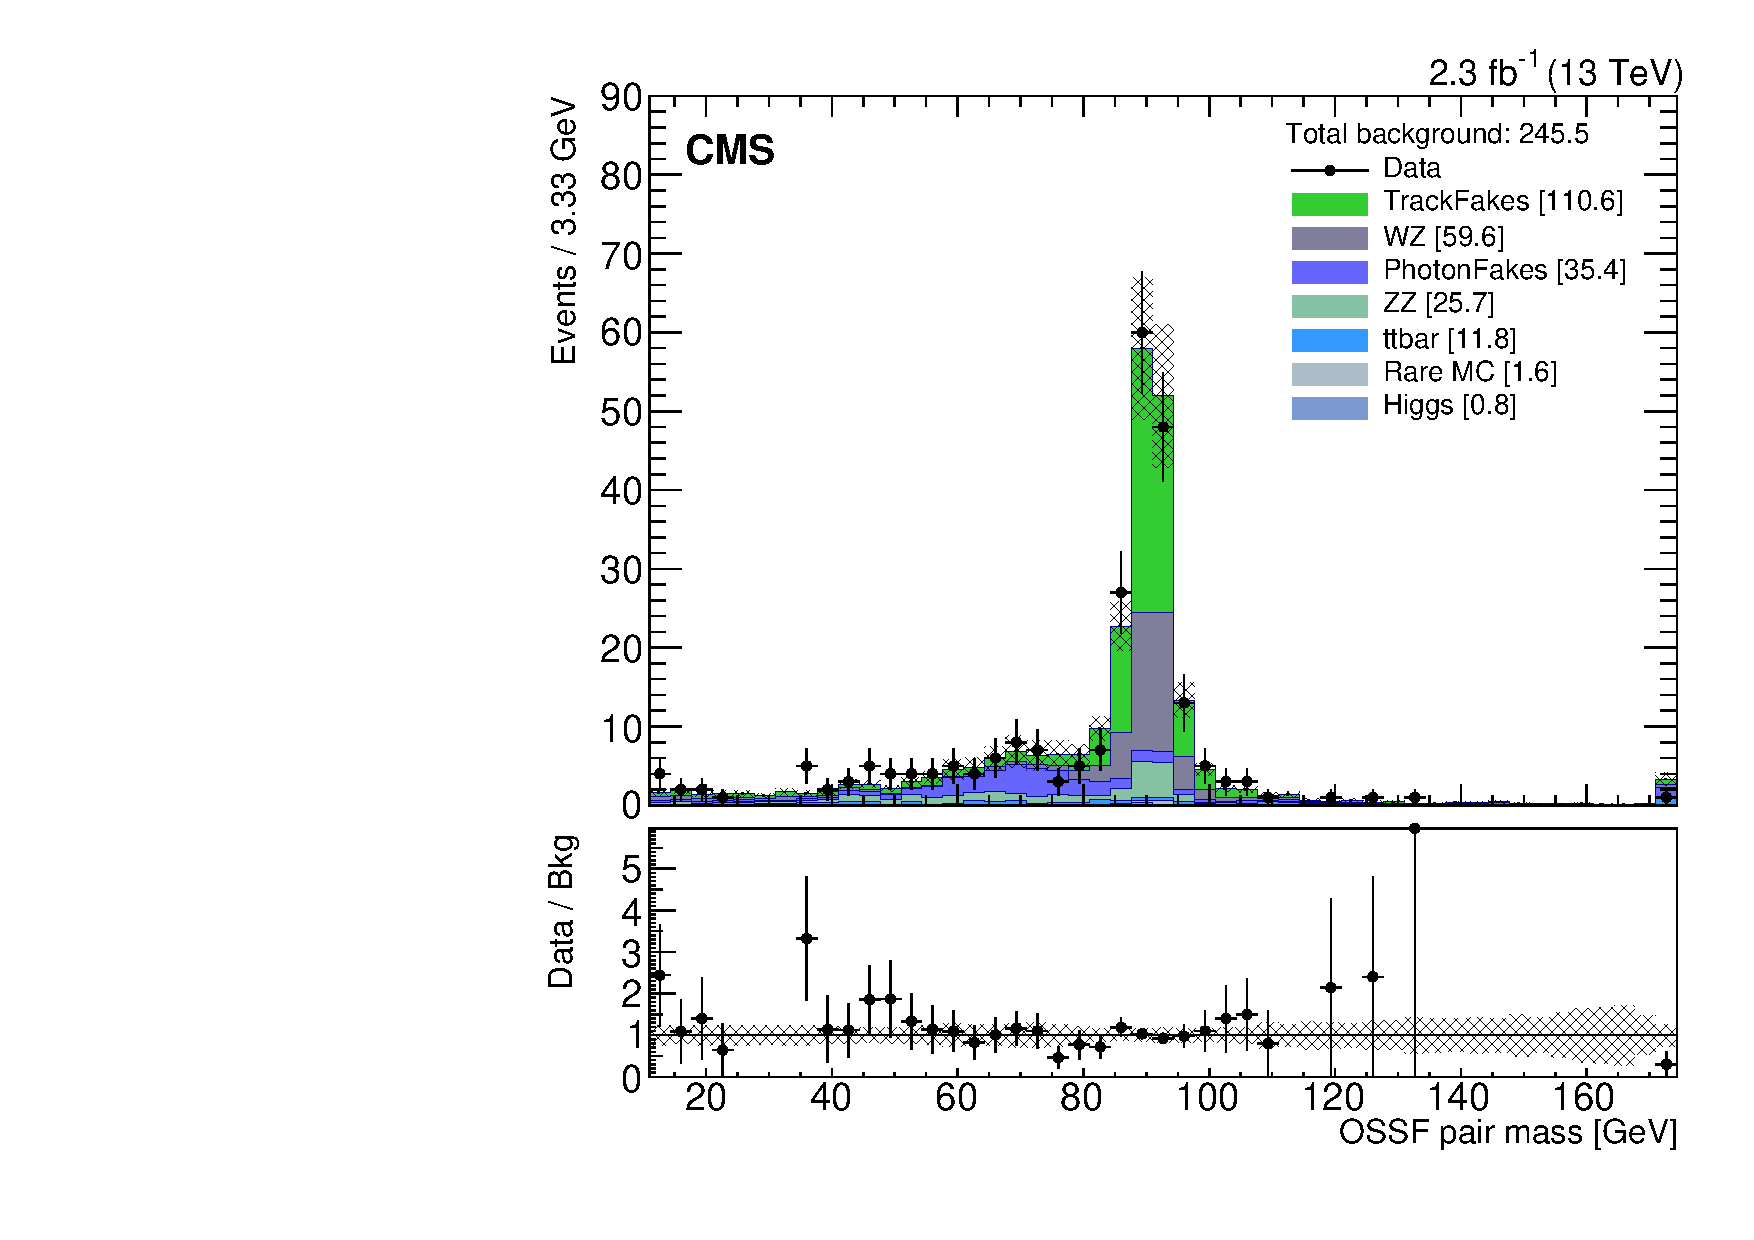
\includegraphics[width=\textwidth]{Background/bkg_fakeLight/Z_2el1mu_MOSSF}
		\caption{$\mu$ fake, $\Z \to e e$}
	\end{subfigure}%
	\caption{$m_{\ell\ell}$ distribution in the dilepton + fake region by flavor.
	\label{fig:fakeLight_Z_MOSSF_byFlavor}}
\end{center}
\end{figure}

As an additional cross-check, we show the \HT distribution in the \Z region (Fig.~\ref{fig:fakeLight_Z_HT}).
\begin{figure}
\begin{center}
	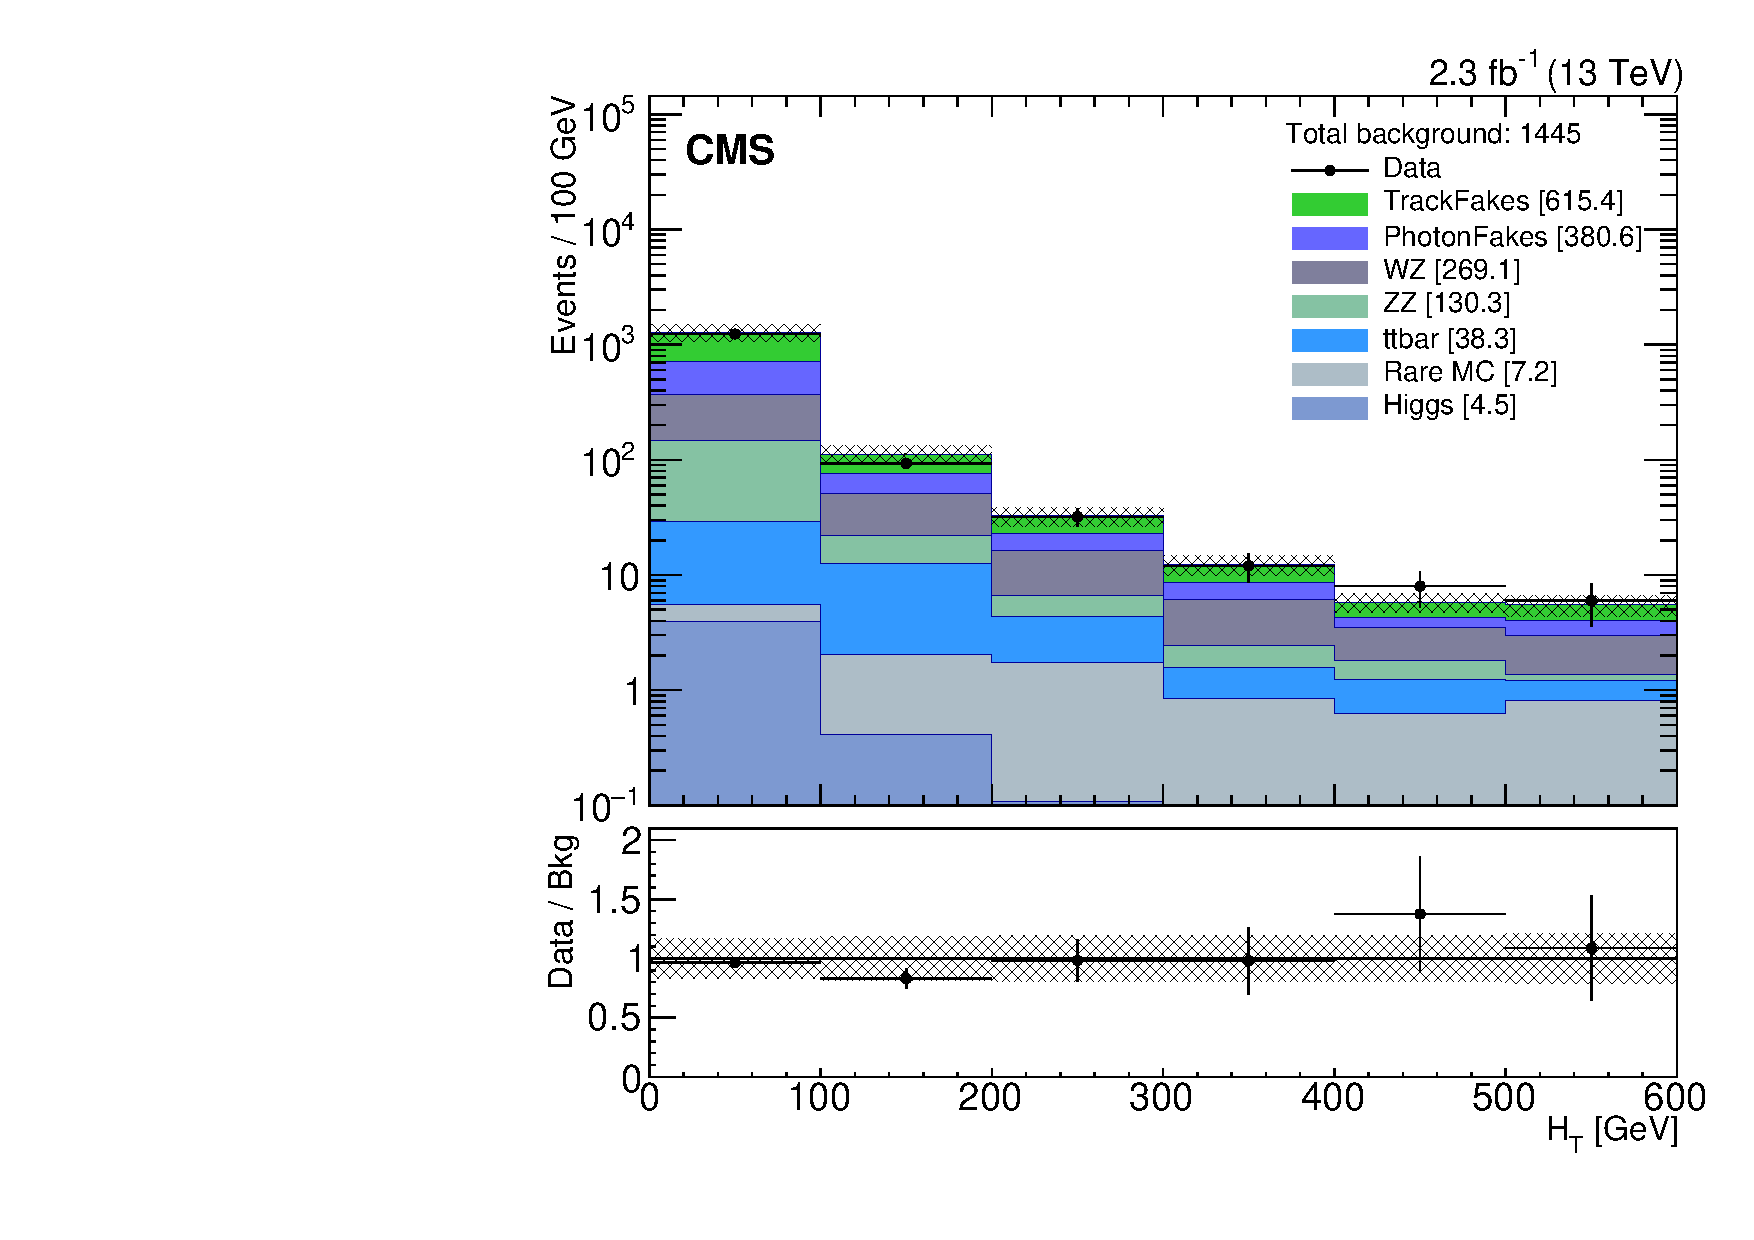
\includegraphics[width=.7\textwidth]{Background/bkg_fakeLight/Z_HT}
	\caption{$\HT$ distribution in the dilepton fake region (no OSSF pair mass cut)
	\label{fig:fakeLight_Z_HT}}
\end{center}
\end{figure}
Finally, we perform a closure test in Drell-Yan MC, comparing the on-Z and off-Z behavior in the control trilepton region (see Fig.~\ref{fig:fakeLight_closure}). We find that the fake rates agree within 5\,\% on and off Z. The statistical uncertainty of the numerator in the high-Z region is 15\,\%.

\begin{figure}
\begin{center}
	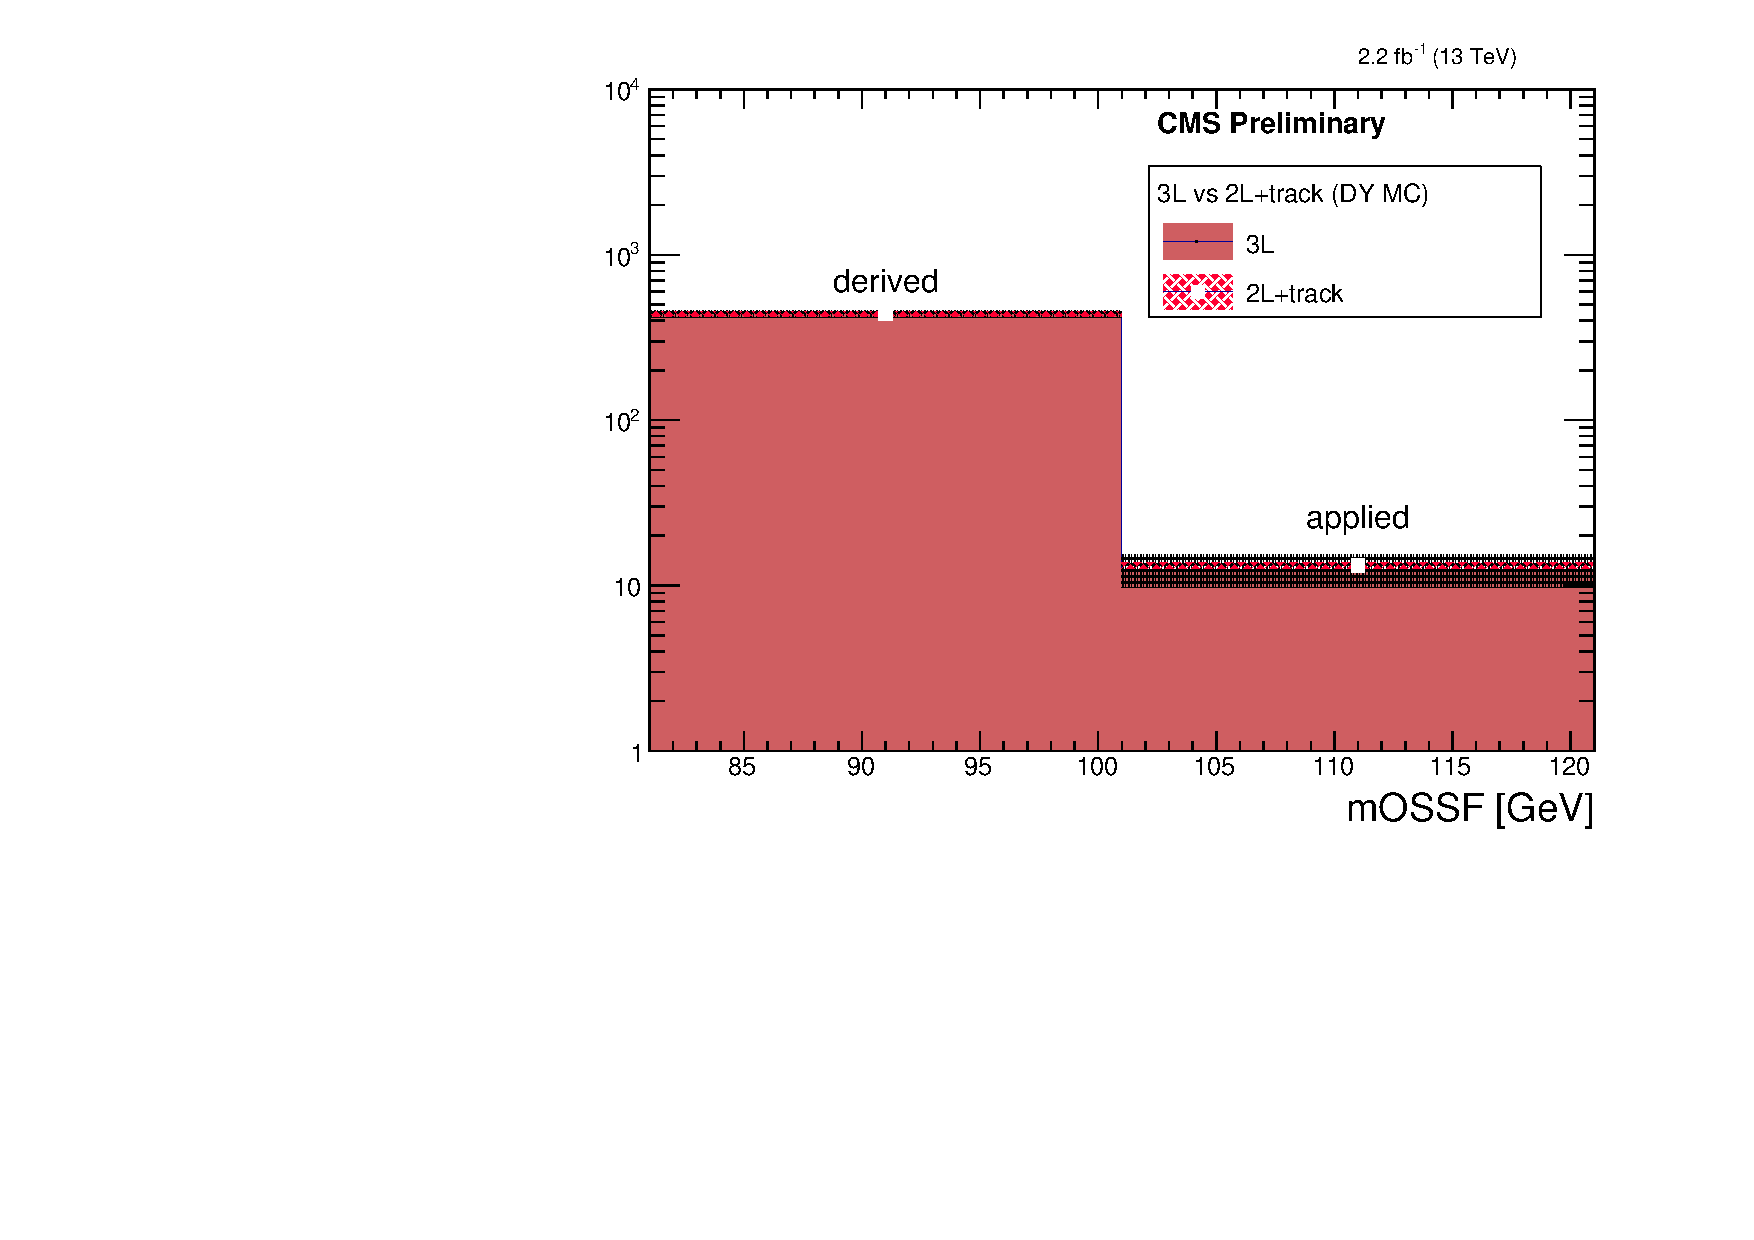
\includegraphics[width=.7\textwidth]{Background/bkg_fakeLight/L3vsL2T1_MOSSF-formatted}
	\caption{Closure test in Drell-Yan MC for the track-based fake rate method. The plot compares the 3-lepton yield with the prediction from 2 leptons + track proxy. (The second bin in this plot ranges from 101 GeV to infinity.)
	\label{fig:fakeLight_closure}}
\end{center}
\end{figure}

\section{\texorpdfstring{\ZZ}{ZZ} Background}
\label{sec:bkg_ZZ}

While the \ZZ background is responsible for only 3\,\% of the background in the ten channels with highest overall sensitivity, its contribution is around 40\,\% in the 4-lepton regions.

The control region is defined by 4 leptons, 2 OSSF pairs (at least one on-\Z), and $\MET < 50\,\GeV$. We use \ZZ MC with fully leptonic decays and normalize the total number of events in the control region, after subtracting other backgrounds. The normalization factor is $1.38 \pm 0.23\stat$. Fig.~\ref{fig:ZZ} shows the 4$\ell$ mass distribution in the control region.

\begin{figure}
\begin{center}
	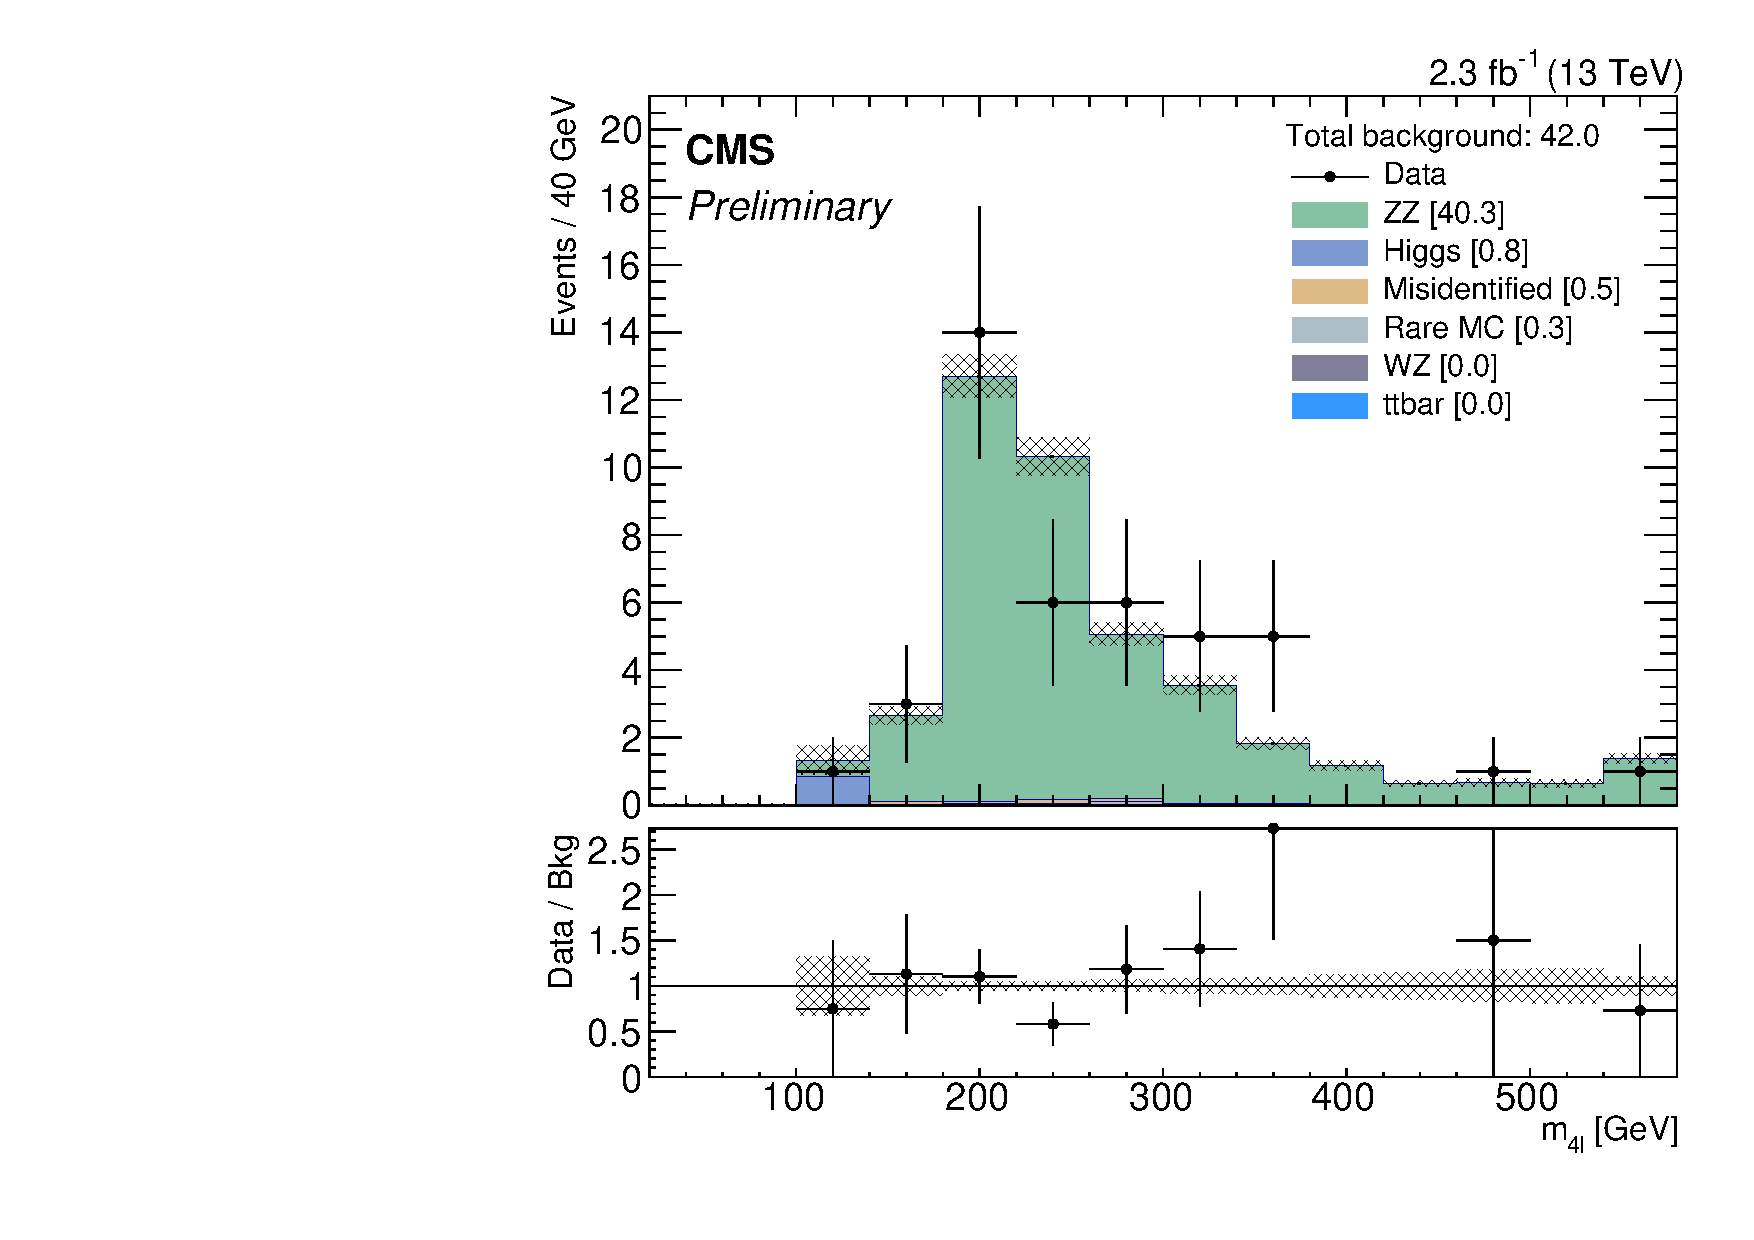
\includegraphics[width=.7\textwidth]{Background/bkg_ZZ/ZZ_DYz2MET0to50HT0to200_MLIGHTLEPTONS}
	\caption{The $m_{4\ell}$ distribution in the \ZZ control region. The last bin is the overflow. Uncertainty bands include both statistical and systematic uncertainties, with the exception of the \ZZ normalization uncertainty.
	\label{fig:ZZ}}
\end{center}
\end{figure}


\chapter{Systematic Uncertainties}
\label{chap:Systematics}

Since most of the signal regions are limited by statistics, systematic uncertainties play a minor role. The only regions where we expect 10 or more events are the signal regions with 3 leptons including an OSSF pair on or above-\Z, and $L_\textrm{T} + \MET < 550\GeV$. In these regions, the \WZ and \ttbar background uncertainties become relevant. However, channels with higher $L_\textrm{T} + \MET$ are more sensitive to the signal. The full list of uncertainties is found in Table~\ref{tab:Systematics}, along with their impact on a representative set of three of the most sensitive channels.

\begin{table}
\centering
\small
\caption{Systematic uncertainties. The channels listed here have three leptons and $550\GeV < L_\textrm{T} + \MET < 750\GeV$.} \label{tab:Systematics}
\begin{tabular}{l c c c c}
\hline\hline
 & & \multicolumn{3}{c}{Impact on background/signal estimate in channel with} \\
Source of uncertainty & Magnitude & no OSSF pair & OSSF pair above-\Z & OSSF pair on-\Z \\
\hline
\WZ normalization                & 50\,\%       & 13\,\%  & 2.8\,\% & 41\,\%  \\
\ZZ normalization                & 16\,\%       & 0.1\,\% & 0.5\,\% & 0.4\,\% \\
Integrated luminosity            & 2.7\,\%      & 0.6\,\% & 0.2\,\% & 0.3\,\% \\
Lepton ID and isolation          &  3\,\%       & 3\,\%   & 3\,\%   & 3\,\%   \\
\MET resolution/smearing         & 50\,\%       & 4.1\,\% & 6.3\,\% & 0.6\,\% \\
Pile-up reweighting              & 5\,\%        & 1.5\,\% & 0.3\,\% & 1.3\,\% \\
\ttbar misidentification rate    & 50\,\%       & 21\,\%  & 11\,\%  & 1.8\,\% \\
\Z + fake background             & 14\,\%       & 9.2\,\% & 1.1\,\% & 1.0\,\% \\
Rare MC cross section            & 50\,\%       & 11\,\%  & 2.7\,\% & 5.2\,\% \\
\\
Signal cross section             & 10\,\%       & 10\,\%  & 10\,\%  & 10\,\% \\
\\
\multicolumn{2}{l}{Total Background (for comparison)} & 0.3 events & 3.0 events & 3.5 events \\
\multicolumn{2}{l}{Signal ($m_\Sigma = 420\GeV$, for comparison)} & 0.8 events & 1.8 events & 0.8 events \\
\hline
\end{tabular}
\end{table}

The \ZZ and \ttbar uncertainties are based on the statistical uncertainties of the normalization regions; cross section uncertainties are thus not applied. For \WZ, we apply a 50\,\% uncertainty to account for the variation of the normalization factor depending on the \MET range chosen for normalization (see Sec.~\ref{sec:bkg_WZ}). For rare background processes, we apply a 50\,\% theory systematic uncertainty to cover both PDF as well as renormalization and factorization scale uncertainties. In the case of the signal, these uncertainties are covered by a 10\,\% systematic uncertainty \cite{CMS-PAS-EXO-14-001}.

For the \MET smearing procedure, a conservative uncertainty is determined by varying the amount of smearing by 50\,\%. Pile-up weights are evaluated by varying the minimzm-bias cross section by 5\,\% and propagating the impact on the pile-up weights through the analysis chain.

In general, systematic uncertainties are found by weighing events up or down or smearing them, then propagating those changes into the various bins of the analysis. The change in the expected backgrounds or signal yields in each bin corresponds to a systematic uncertainty, where we keep track of the relative sign of changes between different bins in order to take correlations and anti-correlations into account. Examples:
\begin{itemize}
	\item The luminosity uncertainty is correlated amongst all samples to which it is applied (i.\,e. MC samples that are not normalized to data). 
	\item As we apply the \MET smearing, events can migrate between $L_\textrm{T} + \MET$ bins. The uncertainty of the correction is thus anti-correlated between those bins. 
	\item An increase of the \WZ normalization by $1\sigma$ leads to a decrease of the measured \Z + jets fake rate, as we subtract \WZ background. Similarly, a $1\sigma$ increase of the \Z + jets fake rate leads to a decrease in the \WZ normalization, as the two control regions cannot be completely isolated from each other and have a (small) overlap. In all these cases, we take the relative signs of the changes into account to keep track of the correlations and anti-correlations.
\end{itemize}

Details on the fake rate uncertainties can be found in Sec.~\ref{sec:bkg_fakeLight}.

\chapter{Results}
\label{chap:Results}

\section{Observation}

As described in Sec.~\ref{sec:Optimization} above, the $L_\textrm{T} + \MET$ variable is a very efficient discriminator between the seesaw signal and the SM background. Therefore, the only requirement for the seesaw signal candidate events beyond the preliminary selection described in Sec.~\ref{sec:Selection} is that their $L_\textrm{T} + \MET$ value exceed 350\,\GeV. In Fig.~\ref{fig:Results} we present the $L_\textrm{T} + \MET$ distribution for four event categories as follows: 3 leptons with OSSF pair on-Z; 3 leptons with OSSF pair above-Z; 3 leptons with no OSSF pair; 4 leptons with at least one OSSF pair. Displays of the seesaw signal for heavy fermion mass $m_\Sigma = 420\,\GeV$ are also shown for each category. The signal generally stands out for higher values of $L_\textrm{T} + \MET$, as is to be expected for a massive parent particle. The SM background decomposition is also shown for each category.

\begin{sidewaysfigure}
\begin{center}
	\begin{subfigure}[b]{.5\textwidth}
		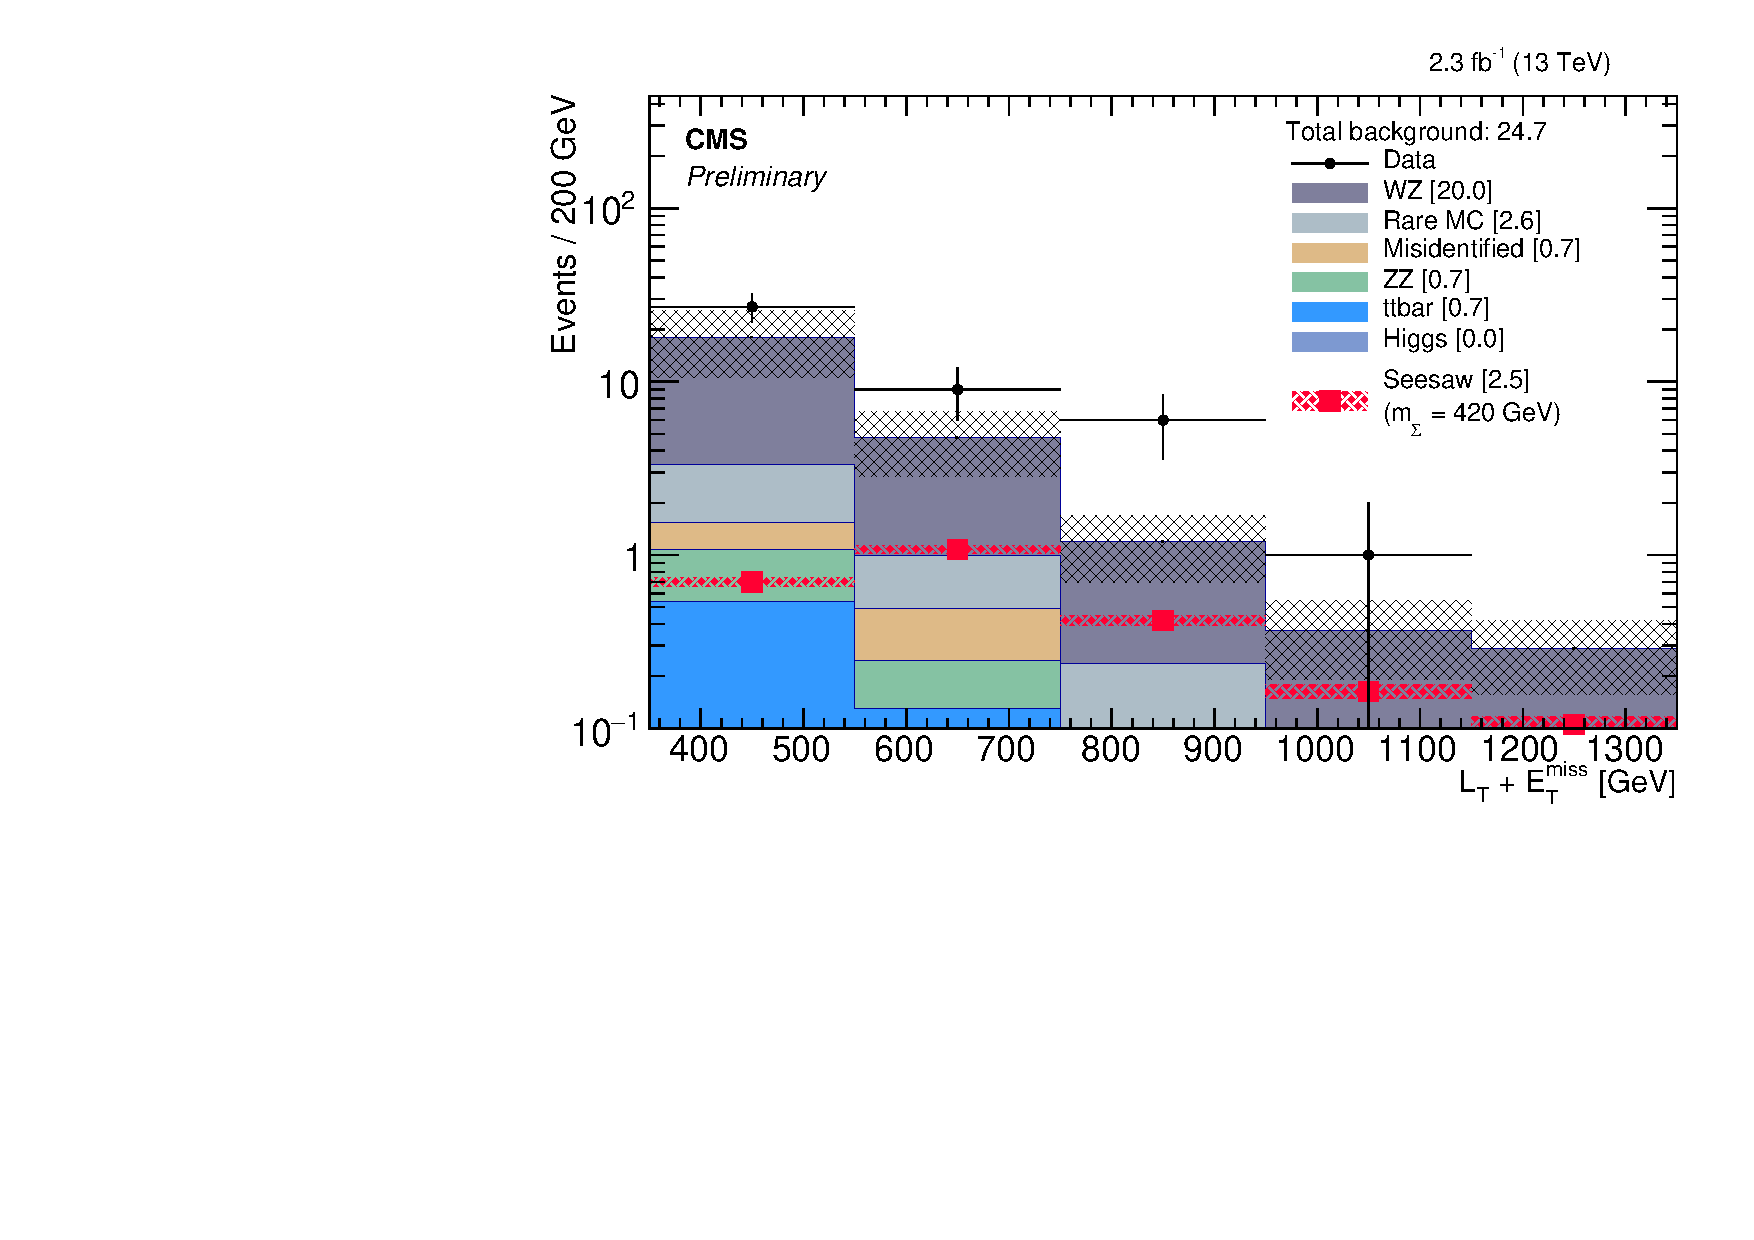
\includegraphics[width=\textwidth]{Results/plots/L3DYz1}
		\caption{3 leptons with OSSF pair on-\Z} \label{fig:Results/a}
	\end{subfigure}%
	\begin{subfigure}[b]{.5\textwidth}
		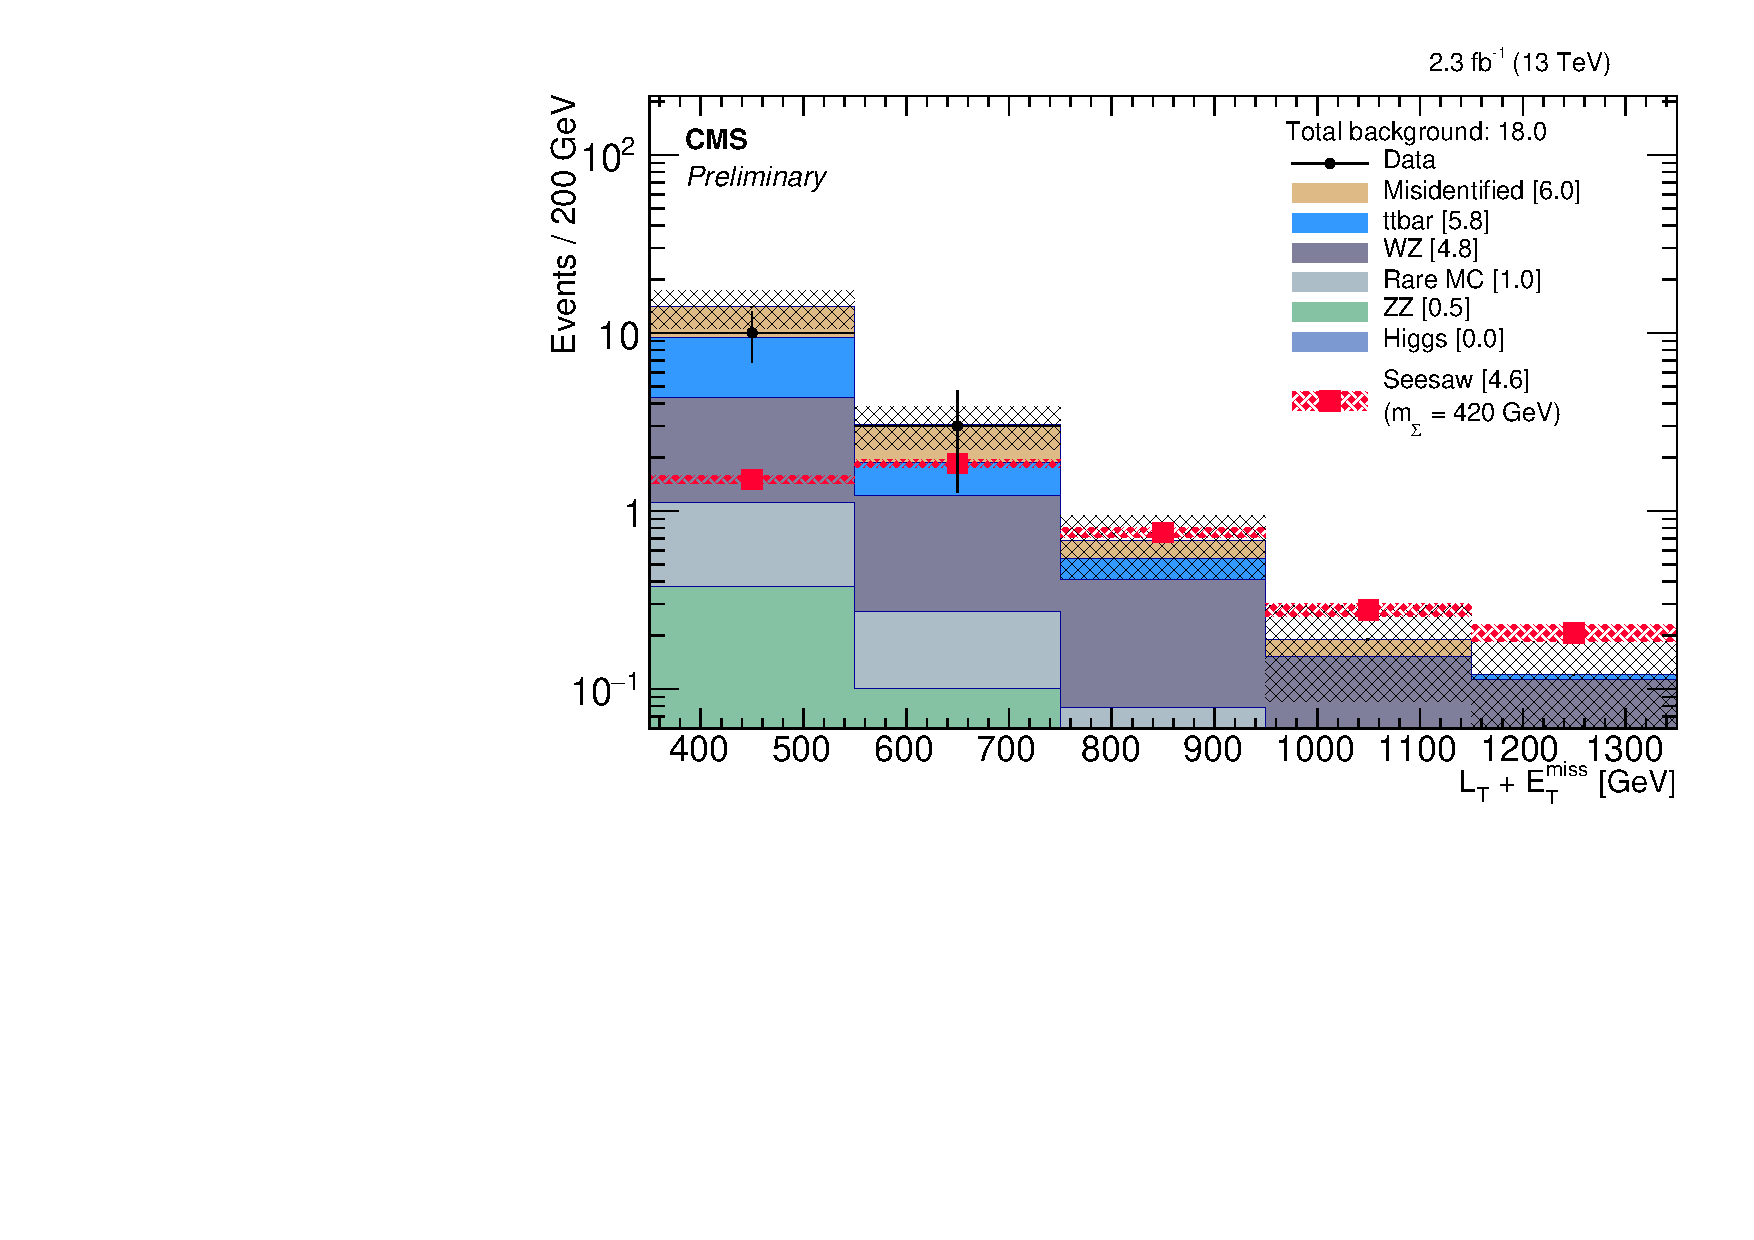
\includegraphics[width=\textwidth]{Results/plots/L3DYh1}
		\caption{3 leptons with OSSF pair above-\Z}
	\end{subfigure}
	\begin{subfigure}[b]{.5\textwidth}
		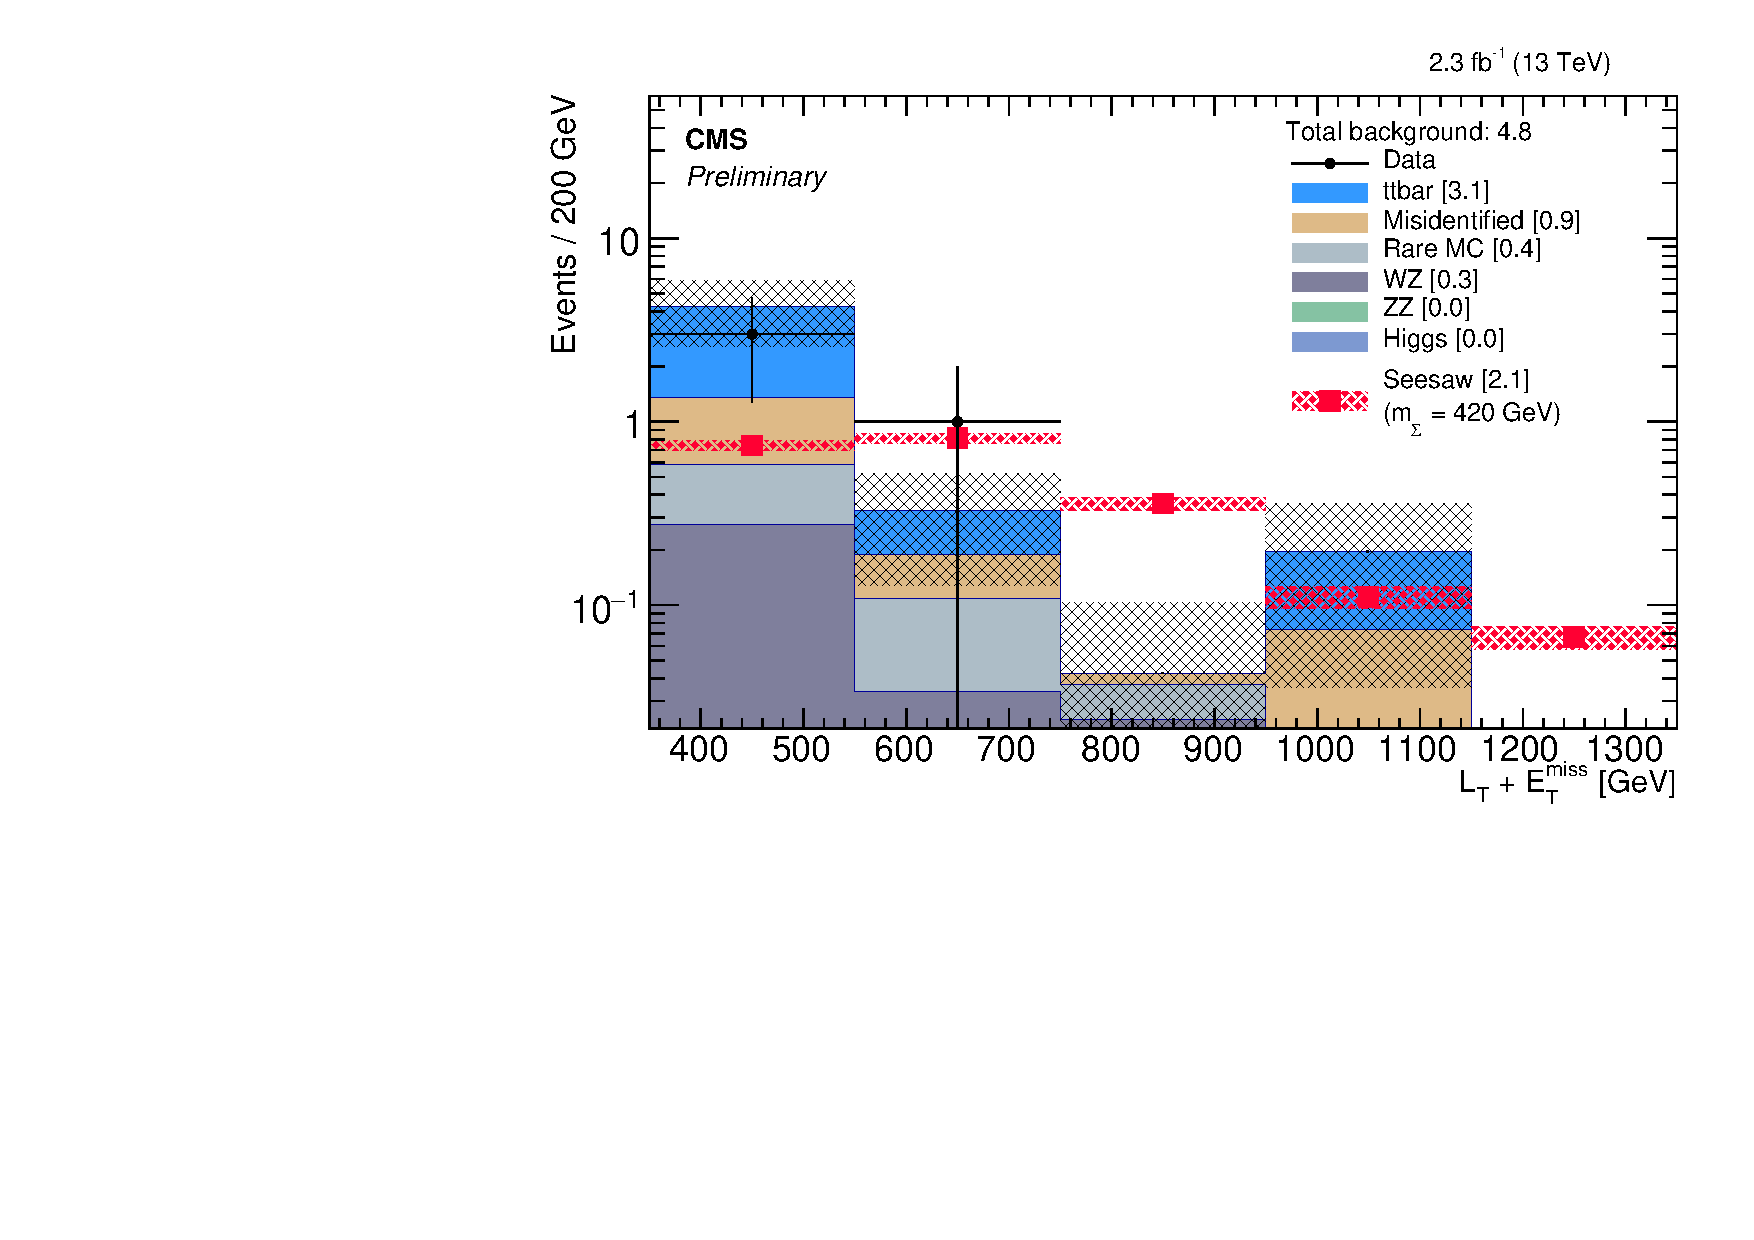
\includegraphics[width=\textwidth]{Results/plots/L3DY0}
		\caption{3 leptons, no OSSF pair}
	\end{subfigure}%
	\begin{subfigure}[b]{.5\textwidth}
		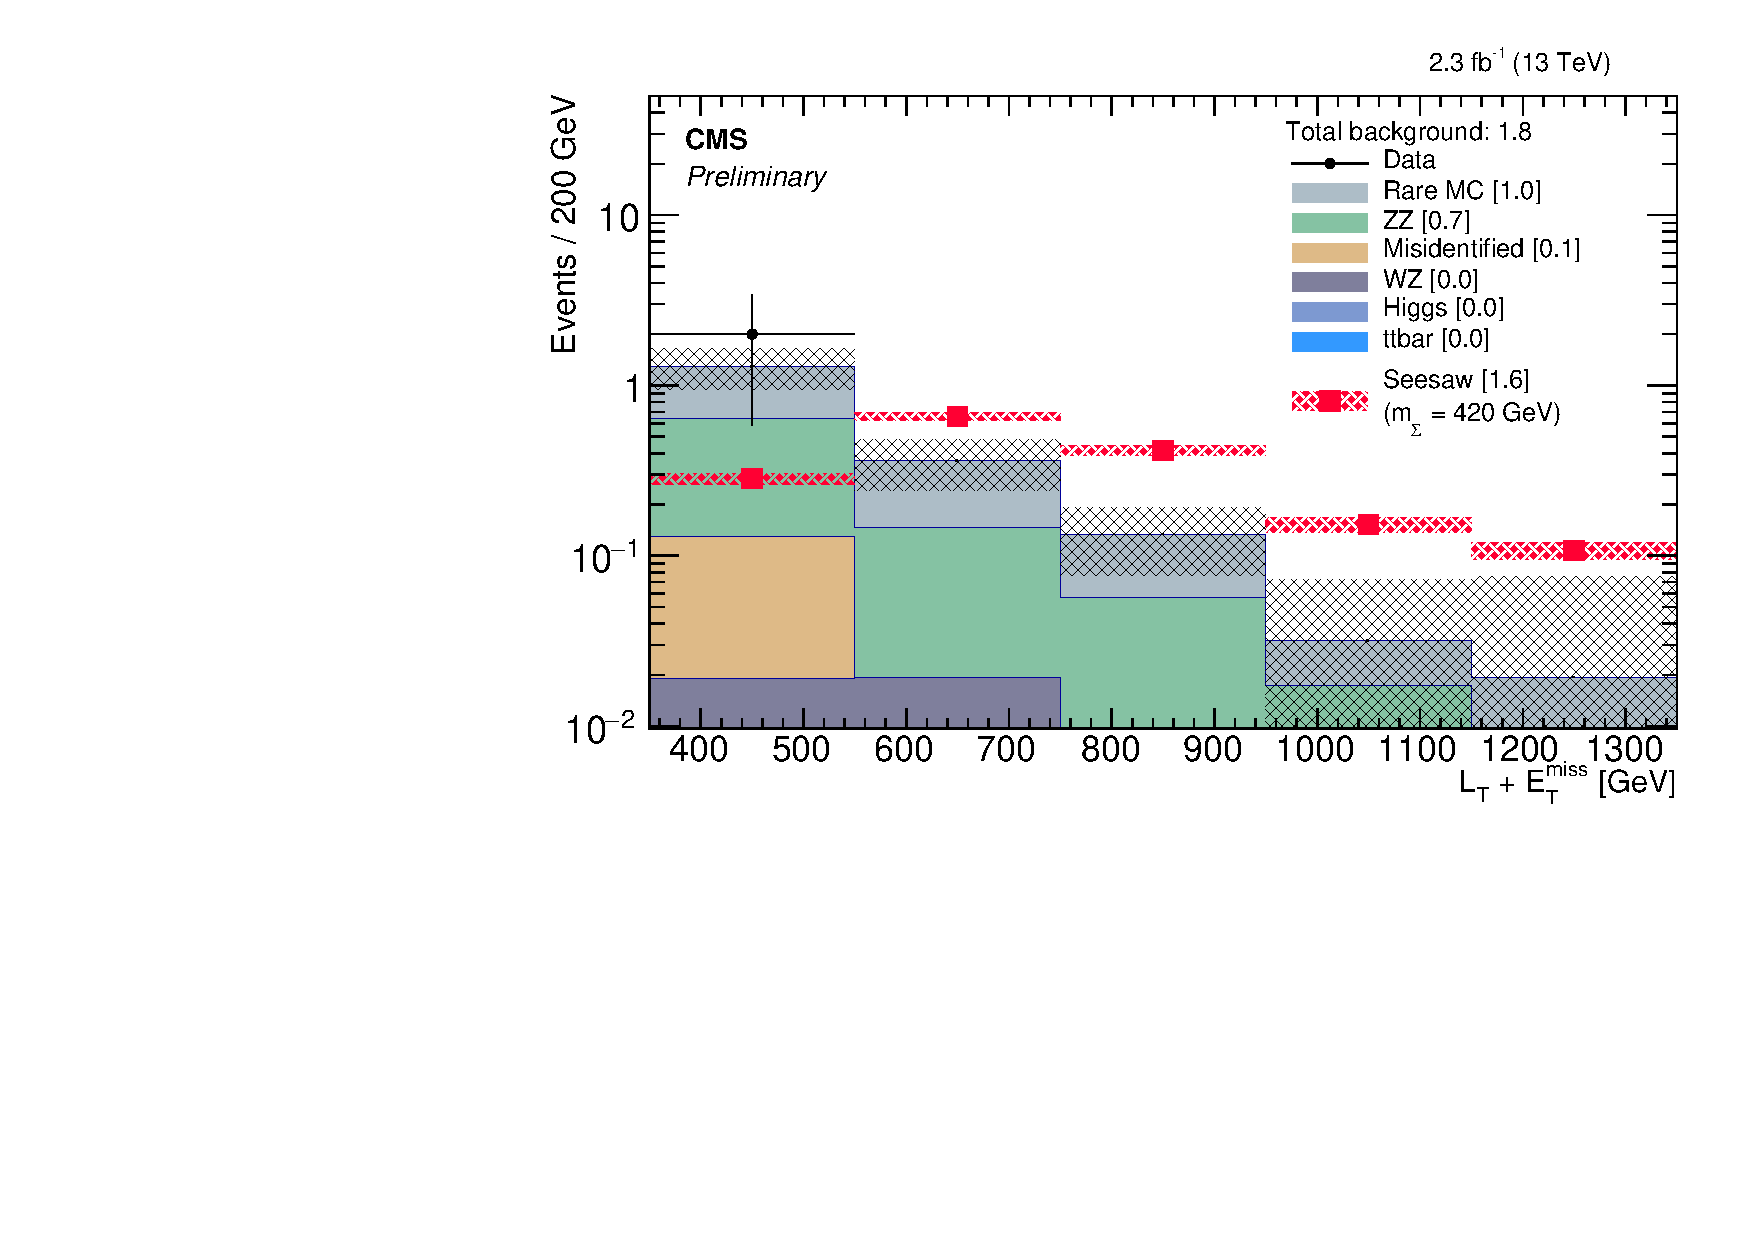
\includegraphics[width=\textwidth]{Results/plots/L4DYgt0}
		\caption{4 leptons, at least 1 OSSF pair}
	\end{subfigure}%
	\caption{Results: $L_\textrm{T} + \MET$ distributions (last bin includes overflow in all plots).
	\label{fig:Results}}
\end{center}
\end{sidewaysfigure}

The observations are consistent with the SM expectations, with the possible exception of the 3-lepton category that includes an OSSF lepton pair with invariant mass consistent with that of the Z boson (Fig.~\ref{fig:Results/a}). The dominant background for this category is the \WZ diboson production, as shown. The $p$-value for the observation in the aggregated twenty $L_\textrm{T} + \MET$ bins for the four categories shown in Fig.~\ref{fig:Results}, assuming SM physics only, is 0.93. This overall consistency with the SM expectation conveys the message that the apparent excess of observed events in the Fig.~\ref{fig:Results/a} is either a statistical artifact or a discrepancy that can be addressed only with additional data.

\section{Interpretation for the Seesaw Model}
\label{sec:Interpretation}
\label{sec:Interpretation/Seesaw}

As no statistically significant excess was observed, we calculate expected and observed upper limits on the cross section sum for the production of seesaw heavy fermion pairs ($\Sigma^0\Sigma^+$, $\Sigma^0\Sigma^-$, or $\Sigma^+\Sigma^-$), assuming a flavor-democratic value for the mixing angle parameters, $V_e = V_\mu = V_\tau = 10^{-6}$, and degenerate heavy fermion masses $m_\Sigma$. The calculation is done using asymptotic CL$_s$ limits with a confidence level of 95\,\% \cite{Junk:1999kv,Read:2000ru,Read:2002hq}.
%Taking the ratio of the cross section upper limit and the signal cross section, one obtains the so-called $r$-value which indicates whether the signal at hand is excluded ($r < 1$) or cannot be excluded ($r > 1$).

If the data agreed perfectly with the background estimates, we would expect our analysis to exclude type-III seesaw heavy fermion pair production for masses below $m_\Sigma = 430\,\GeV$. The observed limit is at 440\,\GeV. While it lags the expected value, the difference is within the uncertainty range because the event category that shows apparent excess as discussed above is not very sensitive to the seesaw signal (Fig.~\ref{fig:Results/a}). The full exclusion curve is shown in Fig.~\ref{fig:exclusion}.

\begin{figure}[t]
\begin{center}
	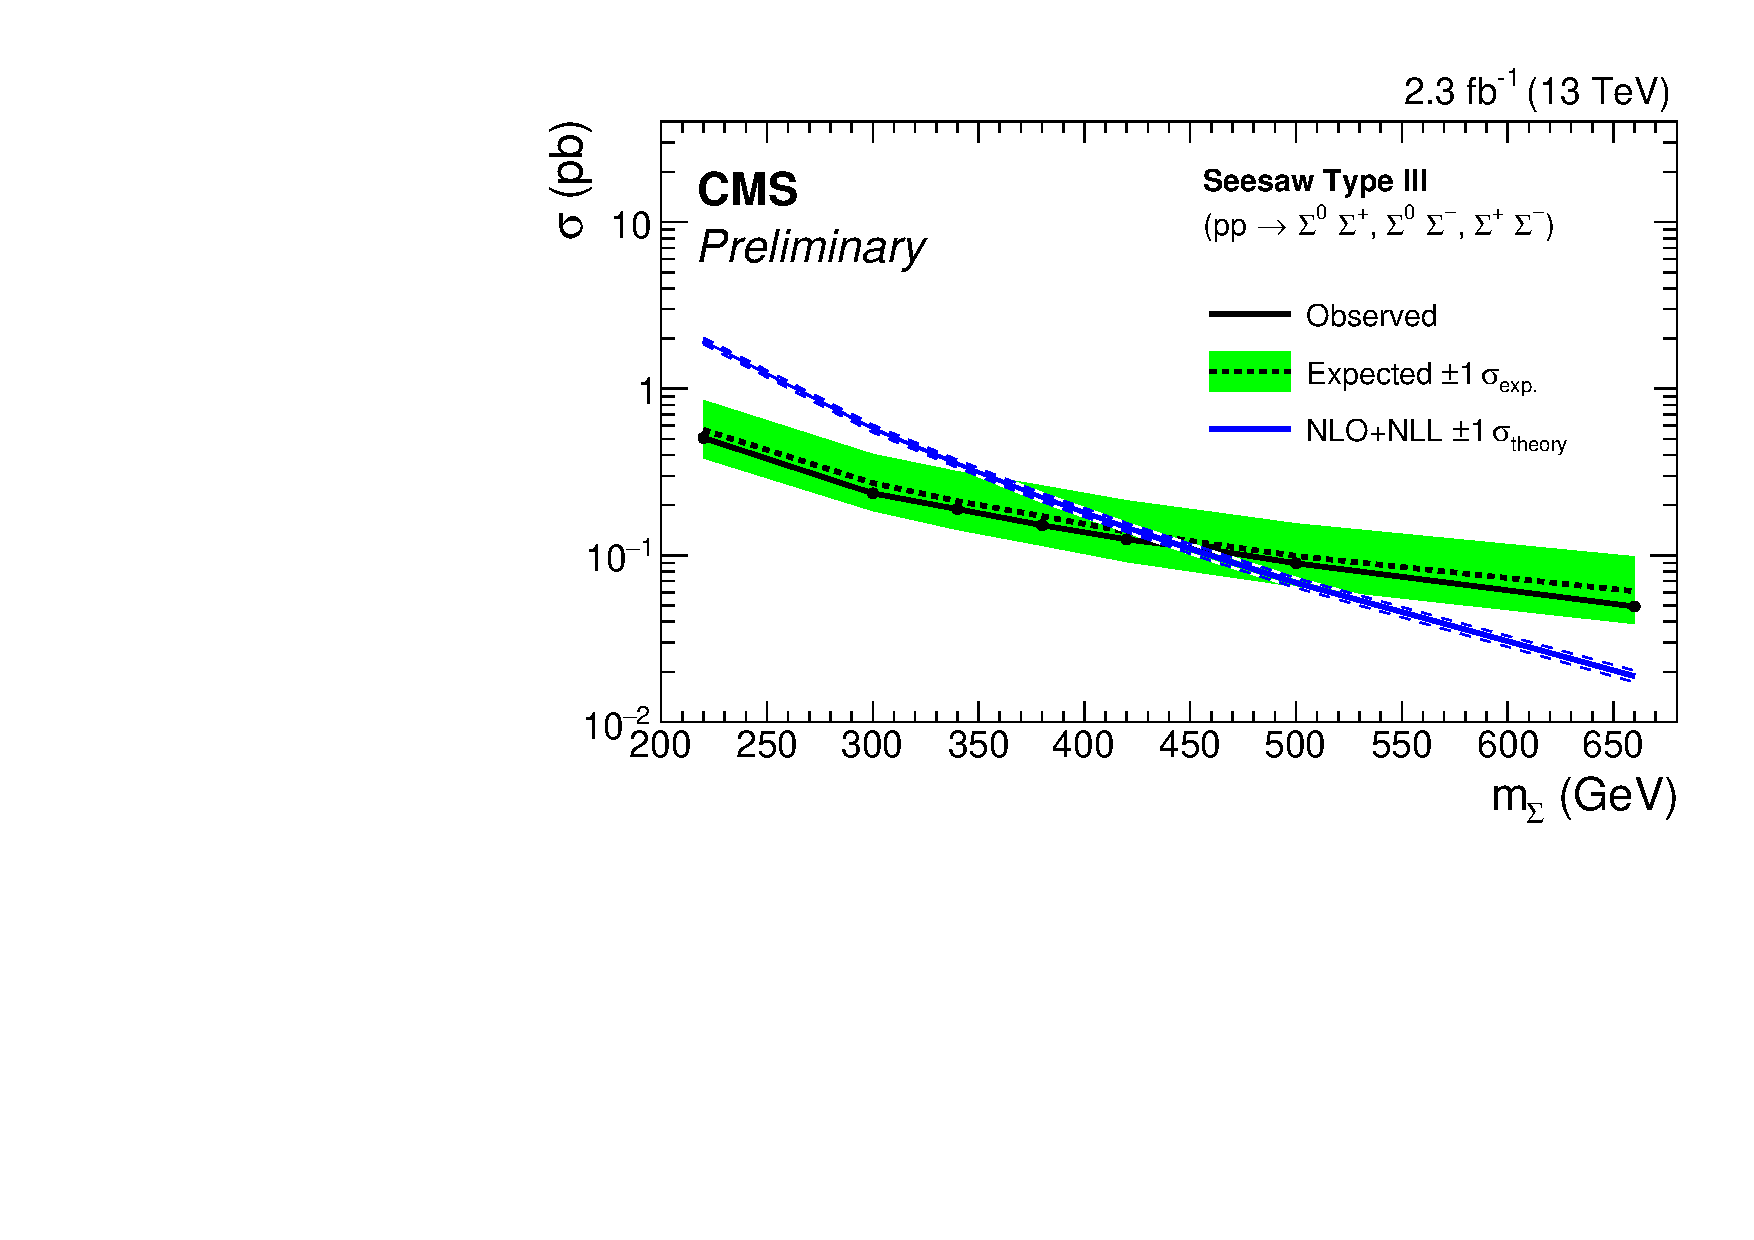
\includegraphics[width=.8\textwidth]{Results/exclusion}
	\caption{Exclusion for the flavor-democratic type-III seesaw model ($V_e = V_\mu = V_\tau = 10^{-6}$). We exclude heavy fermion pair production for masses below $m_\Sigma = 440\,\GeV$ (expected: 430\,\GeV) and give upper limits on the pair production cross section.
	\label{fig:exclusion}}
\end{center}
\end{figure}

In comparison to the Run-I results, the search sensitivity has been enhanced by various improvements, most notably the inclusion of new decay modes involving the Higgs boson and of 4-lepton channels, as well as by the introduction of an improved fine-grained binning scheme. Exclusion limits from the CMS Run I result were at $m_\Sigma = 250\,\GeV$ (expected) and $m_\Sigma = 278\,\GeV$ (observed) \cite{CMS-PAS-EXO-14-001}.

\chapter{Interpretation for the Seesaw Model}
\label{sec:Interpretation}
\label{sec:Interpretation/Seesaw}

As no statistically significant excess was observed, we calculate expected and observed upper limits on the cross section sum for the production of seesaw heavy fermion pairs ($\Sigma^0\Sigma^+$, $\Sigma^0\Sigma^-$, or $\Sigma^+\Sigma^-$), assuming a flavor-democratic value for the mixing angle parameters, $V_e = V_\mu = V_\tau = 10^{-6}$, and degenerate heavy fermion masses $m_\Sigma$. The calculation is done using asymptotic CL$_s$ limits with a confidence level of 95\,\% \cite{Junk:1999kv,Read:2000ru,Read:2002hq}.
%Taking the ratio of the cross section upper limit and the signal cross section, one obtains the so-called $r$-value which indicates whether the signal at hand is excluded ($r < 1$) or cannot be excluded ($r > 1$).

If the data agreed perfectly with the background estimates, we would expect our analysis to exclude type-III seesaw heavy fermion pair production for masses below $m_\Sigma = 430\,\GeV$. The observed limit is at 435\,\GeV. While it lags the expected value, the difference is within the uncertainty range because the event category that shows apparent excess as discussed above is not very sensitive to the seesaw signal (Fig.~\ref{fig:Results}a). The full exclusion curve is shown in Fig.~\ref{fig:exclusion}.

\begin{figure}[t]
\begin{center}
	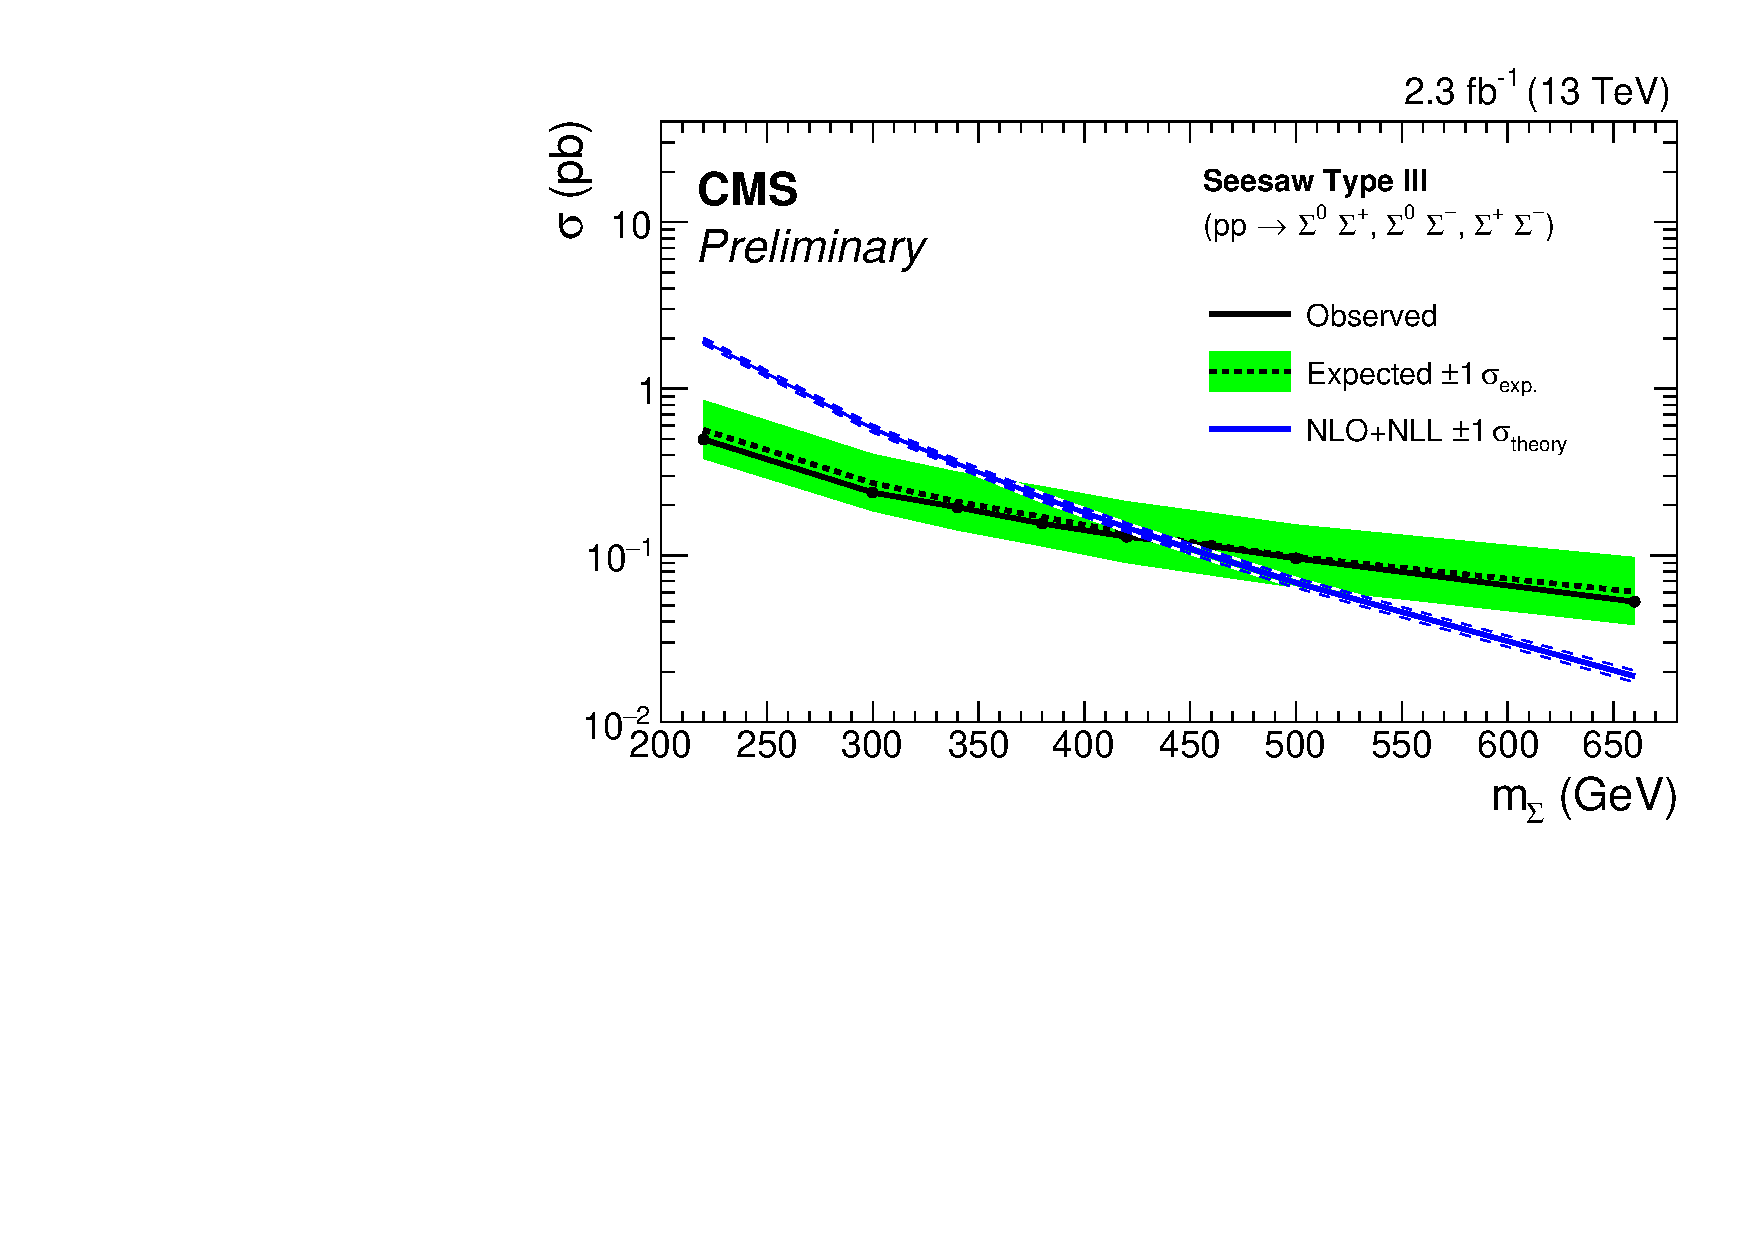
\includegraphics[width=.8\textwidth]{Interpretation/exclusion}
	\caption{Exclusion for the flavor-democratic type-III seesaw model ($V_e = V_\mu = V_\tau = 10^{-6}$). We exclude heavy fermion pair production for masses below $m_\Sigma = 435\,\GeV$ (expected: 430\,\GeV) and give upper limits on the pair production cross section.
	\label{fig:exclusion}}
\end{center}
\end{figure}

In comparison to the Run-I results, the search sensitivity has been enhanced by various improvements, most notably the inclusion of new decay modes involving the Higgs boson and of 4-lepton channels, and by the introduction of an improved fine-grained binning scheme. Exclusion limits from the CMS Run I result were at $m_\Sigma = 250\,\GeV$ (expected) and $m_\Sigma = 278\,\GeV$ (observed) \cite{CMS-PAS-EXO-14-001}.

\chapter{Conclusion}
\label{sec:Summary}

A search for type-III seesaw heavy fermion production has been performed in multilepton final states using \fullLumi of proton--proton collision data at $\sqrt{s} = 13\,\TeV$, collected using the CMS detector at the CERN LHC. No significant discrepancies between the background prediction and the data have been observed. Comparing the data with the predictions, we set upper limits at the 95\,\% confidence level on the production cross section of the heavy fermion pairs. Assuming degenerate heavy fermion masses $m_\Sigma$ in the flavor-democratic scenario, we exclude previously unexplored regions of the signal model with heavy fermion particle masses below $m_\Sigma < 435\,\GeV$ (expected: 430\,\GeV).


\clearpage

%%%%%%%%%%%%%%%%%% Appendix %%%%%%%%%%%%%%%%%%%%
\appendix
\chapter{\texorpdfstring{\Z}{Z} binning}
\label{app:Zbinning}
Note: This section currently has 8 TeV information and has not been updated

\fixme{check interference with MT definition in WZ background section}

We bin events with an OSSF pair depending on whether the pair invariant mass is in the \Z window, or below/above. In case of ambiguity, we need to pick a specific pair. We compare two methods:
\begin{enumerate}
	\item We take the pair whose invariant mass is closest to the \Z mass.
	\item We take the pair closest to the \Z mass, with the additional condition that pairs above the \Z window are not considered if there is a pair below the \Z window (thus shifting events from high-\Z to low-\Z).
\end{enumerate}
Fig.~\ref{fig:app:Zbinning} shows that there is little difference to both approaches. We decide to take the second approach to achieve a more separative categorization of background, especially around the high end of the \Z window.

\begin{figure}
\begin{center}
	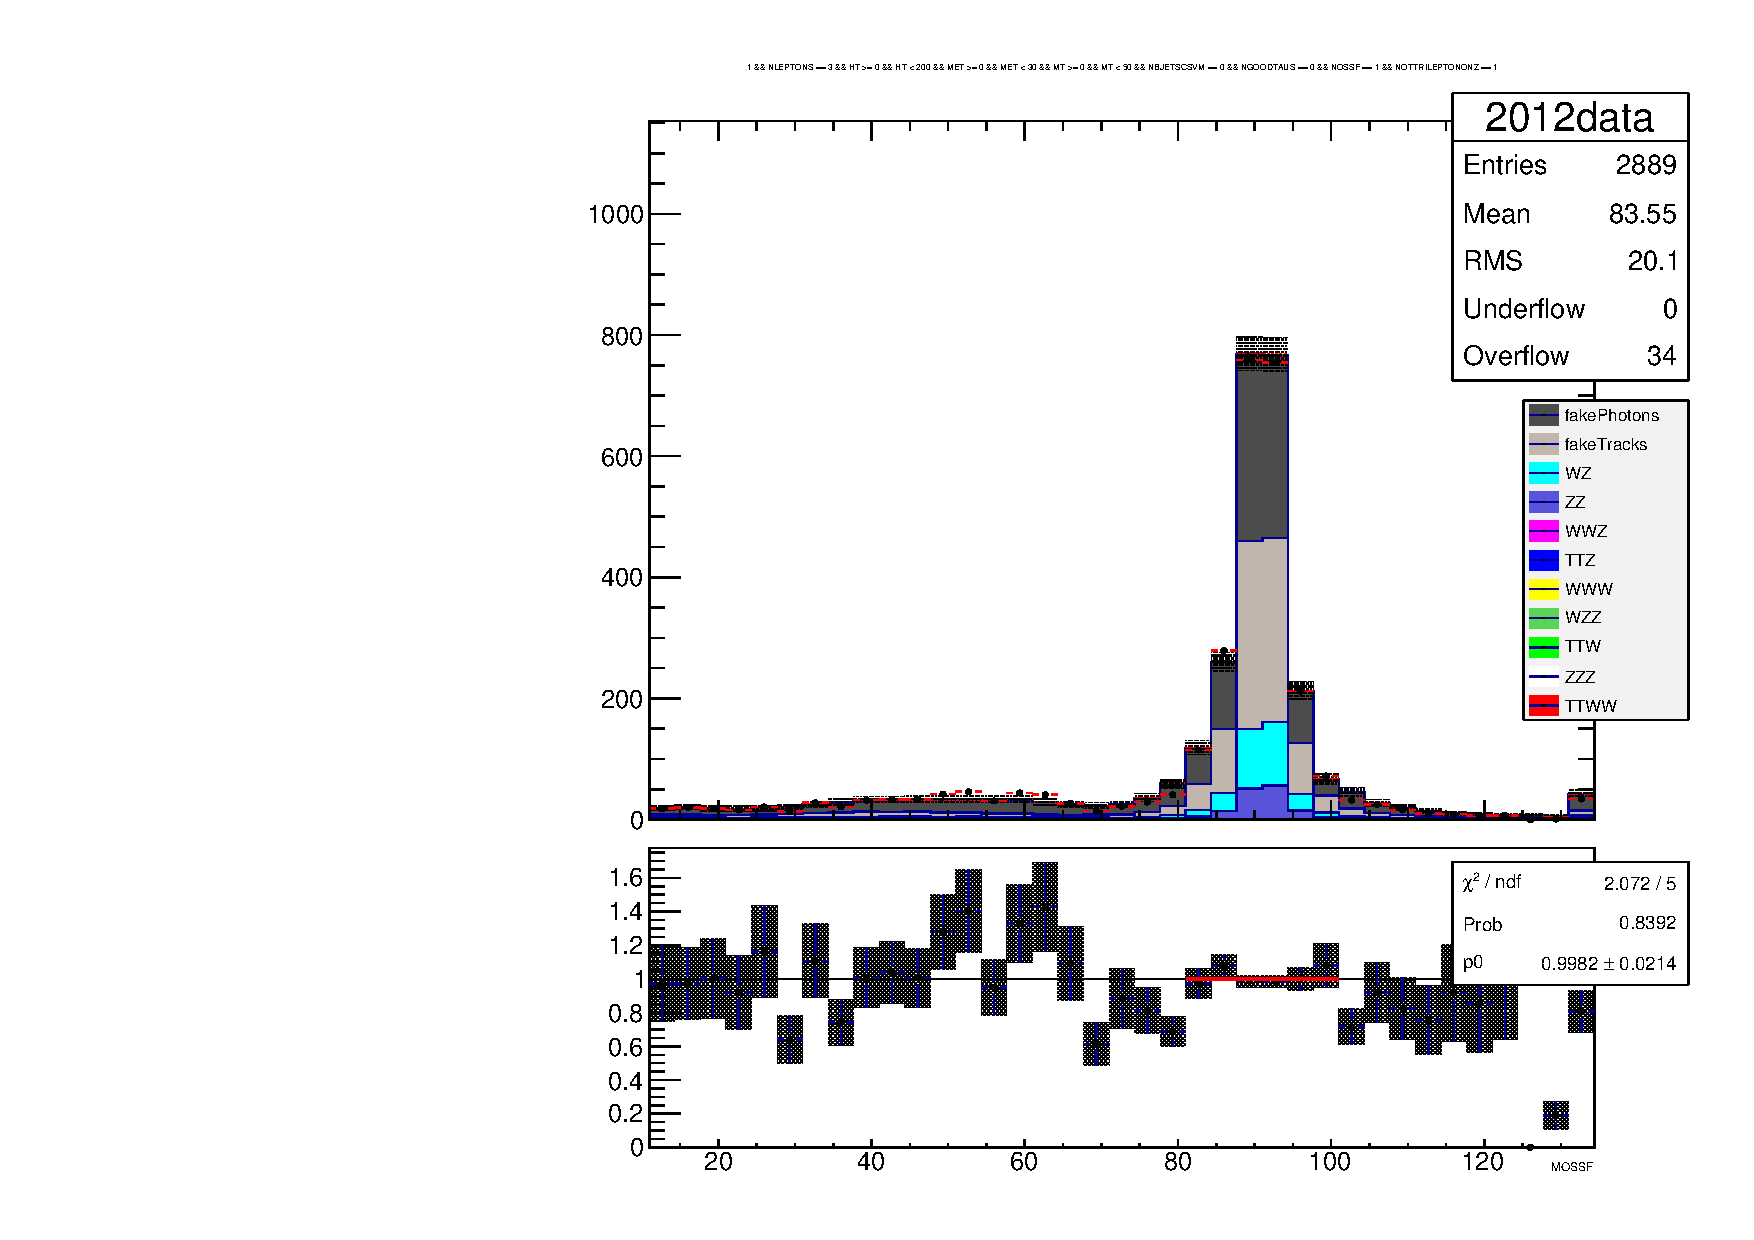
\includegraphics[width=.5\textwidth]{Appendix/Z_NOTTRILEPTONONZ_oldMOSSF}%
	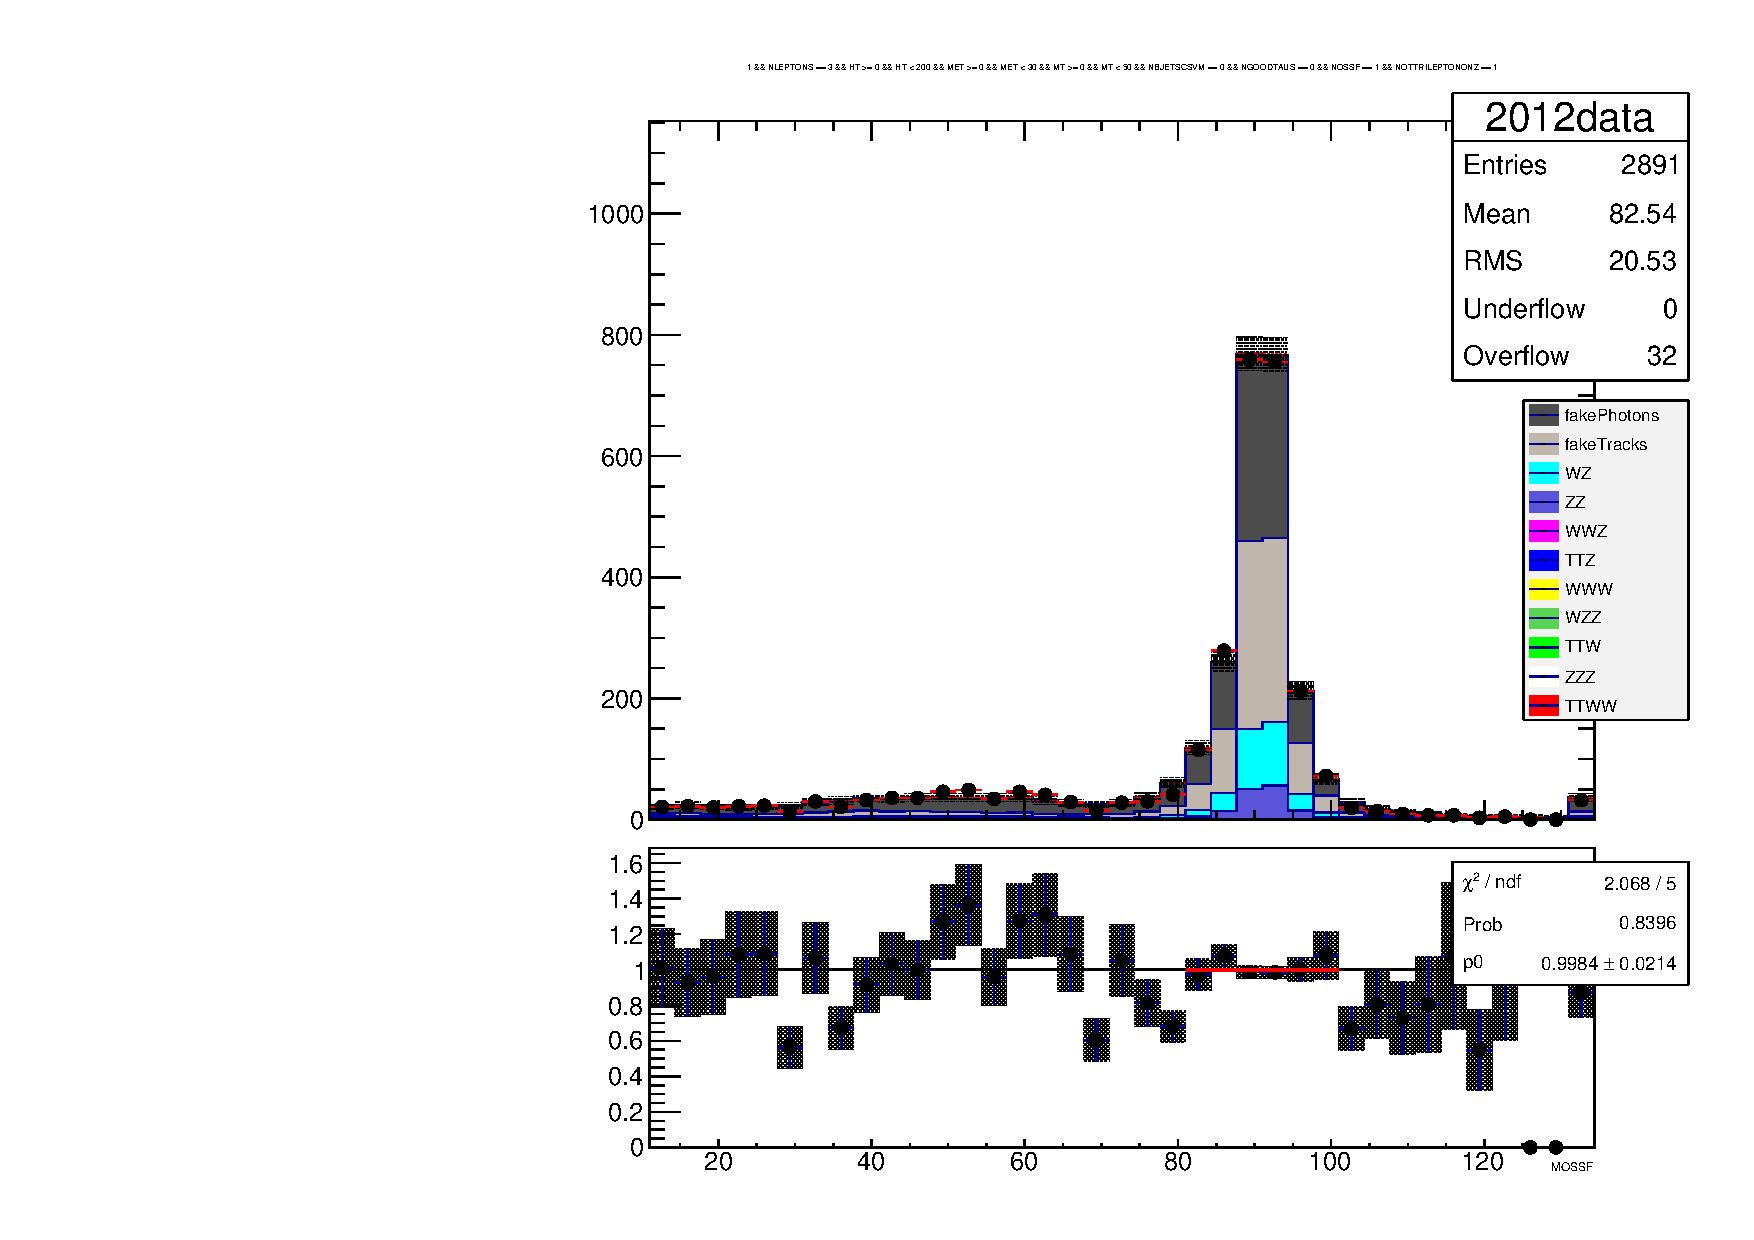
\includegraphics[width=.5\textwidth]{Appendix/Z_NOTTRILEPTONONZ_MOSSF}
	\caption{$m_{\ell\ell}$ distribution in in the dilepton fake region (off-\Z, trilepton events with $m_{\ell\ell\ell}$ on \Z have been vetoed). \enskip left)~method 1 \enskip right)~method 2
	\label{fig:app:Zbinning}}
\end{center}
\end{figure}

\chapter{Suitability of tracks as fake proxies}
\label{app:MOSSFlepton,track}

\subsubsection{Low-quality leptons showing up as tracks}
Note: This section currently has 8 TeV information and has not been updated

Out of curiosity, we look at the invariant mass of an opposite-sign muon+track pair. If the tracks are uncorrelated with the muons, we expect a broad peak at the average invariant mass. If they are correlated, they will be related to their source, for example a \Z decay. In fact, we see both (Figure~\ref{fig:app:MOSSFlepton,track}).

\begin{figure}
\begin{center}
	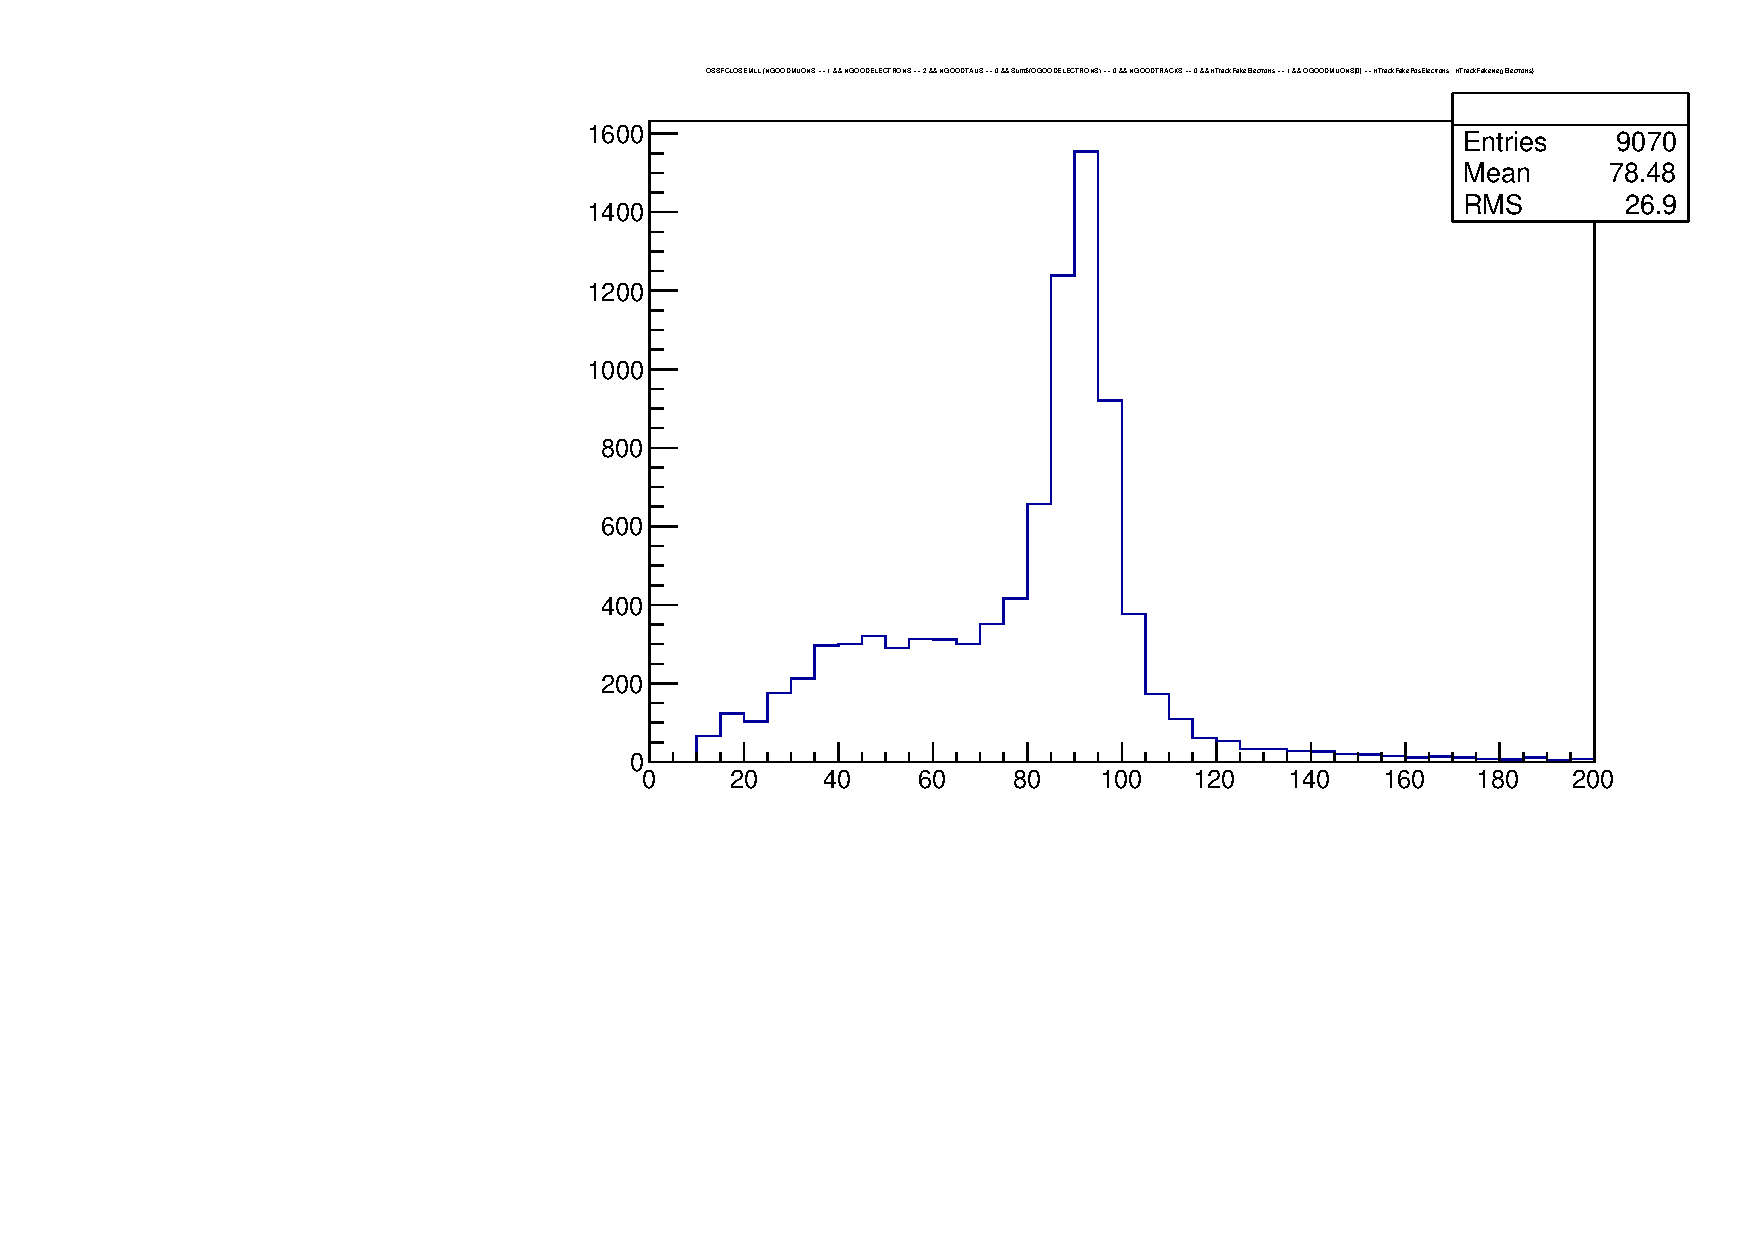
\includegraphics[width=.5\textwidth]{Appendix/study_OSSFCLOSEMLL_electron,track_1fake}%
	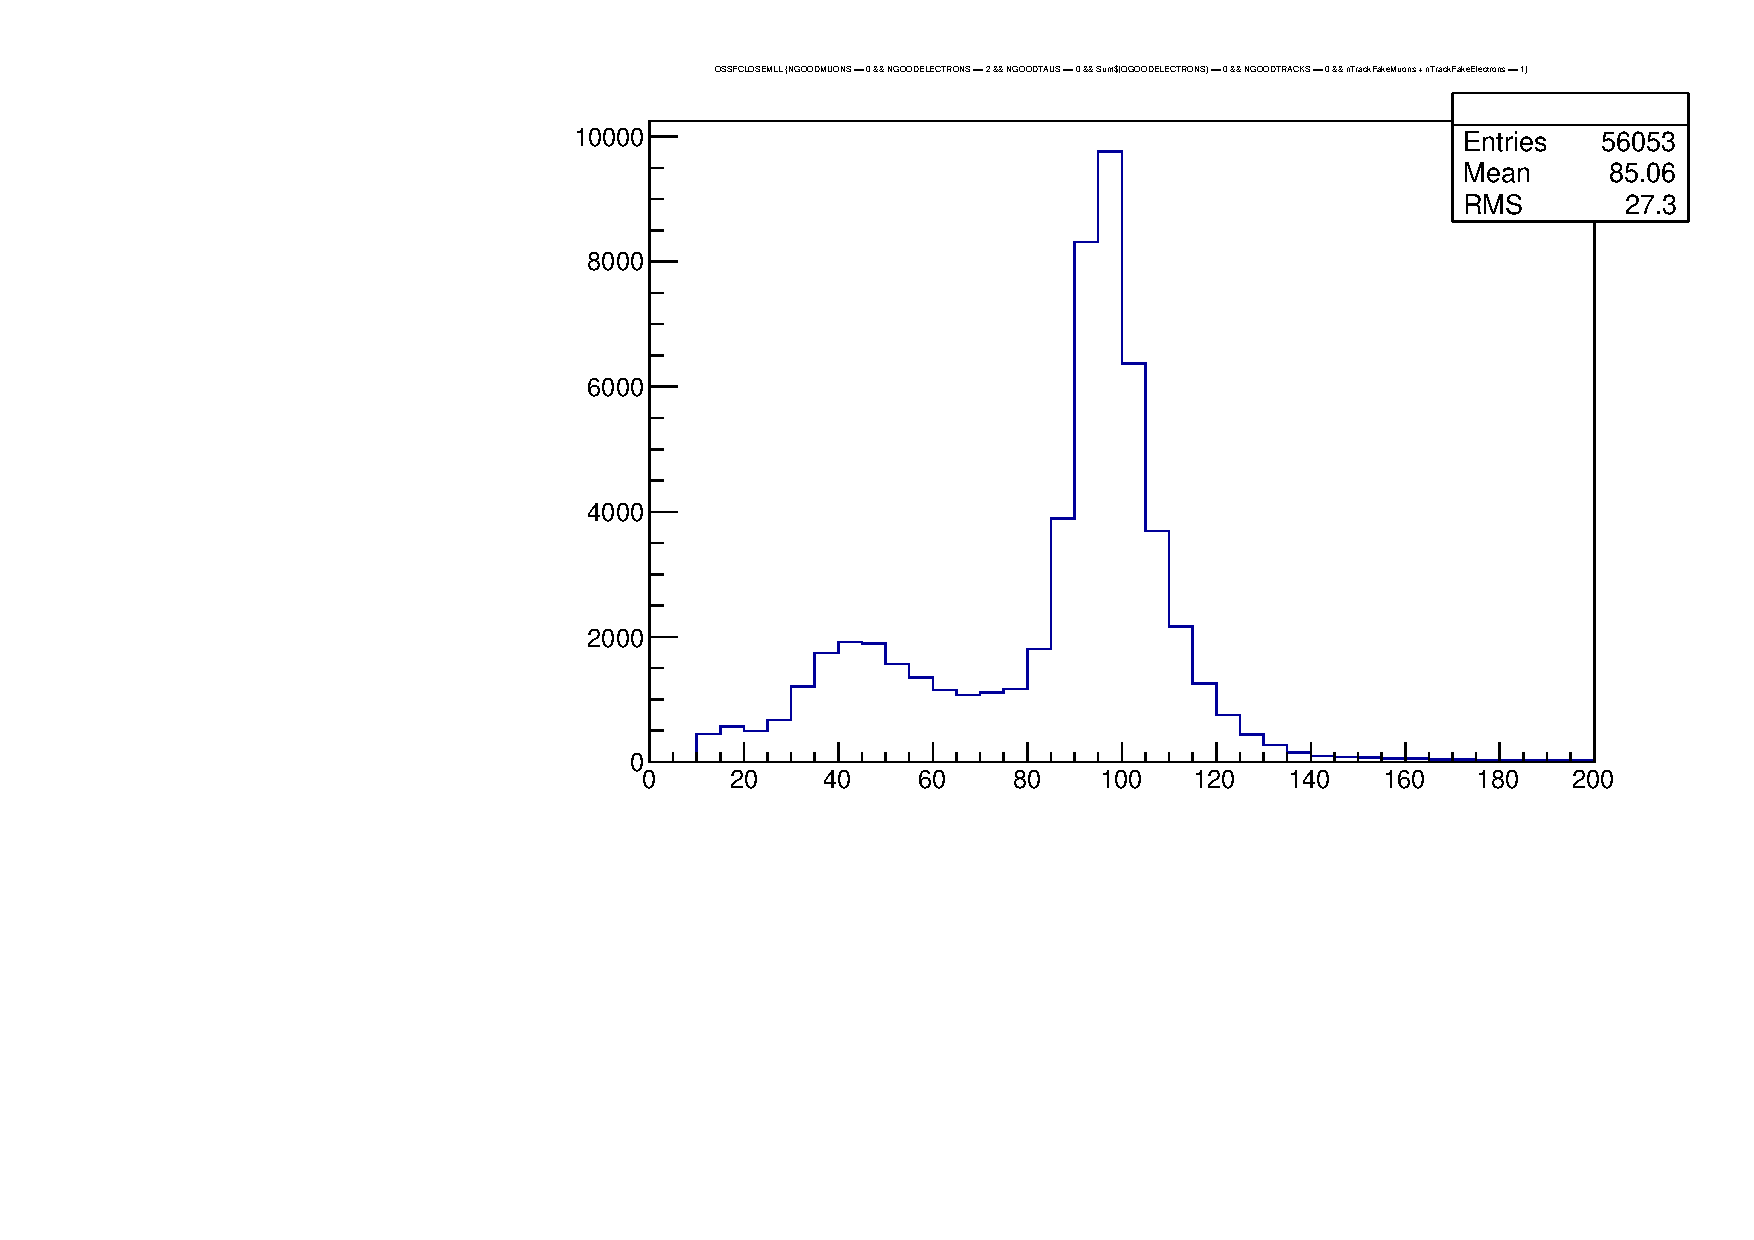
\includegraphics[width=.5\textwidth]{Appendix/study_OSSFCLOSEMLL_electron,track_dileptons-1fake}\\
	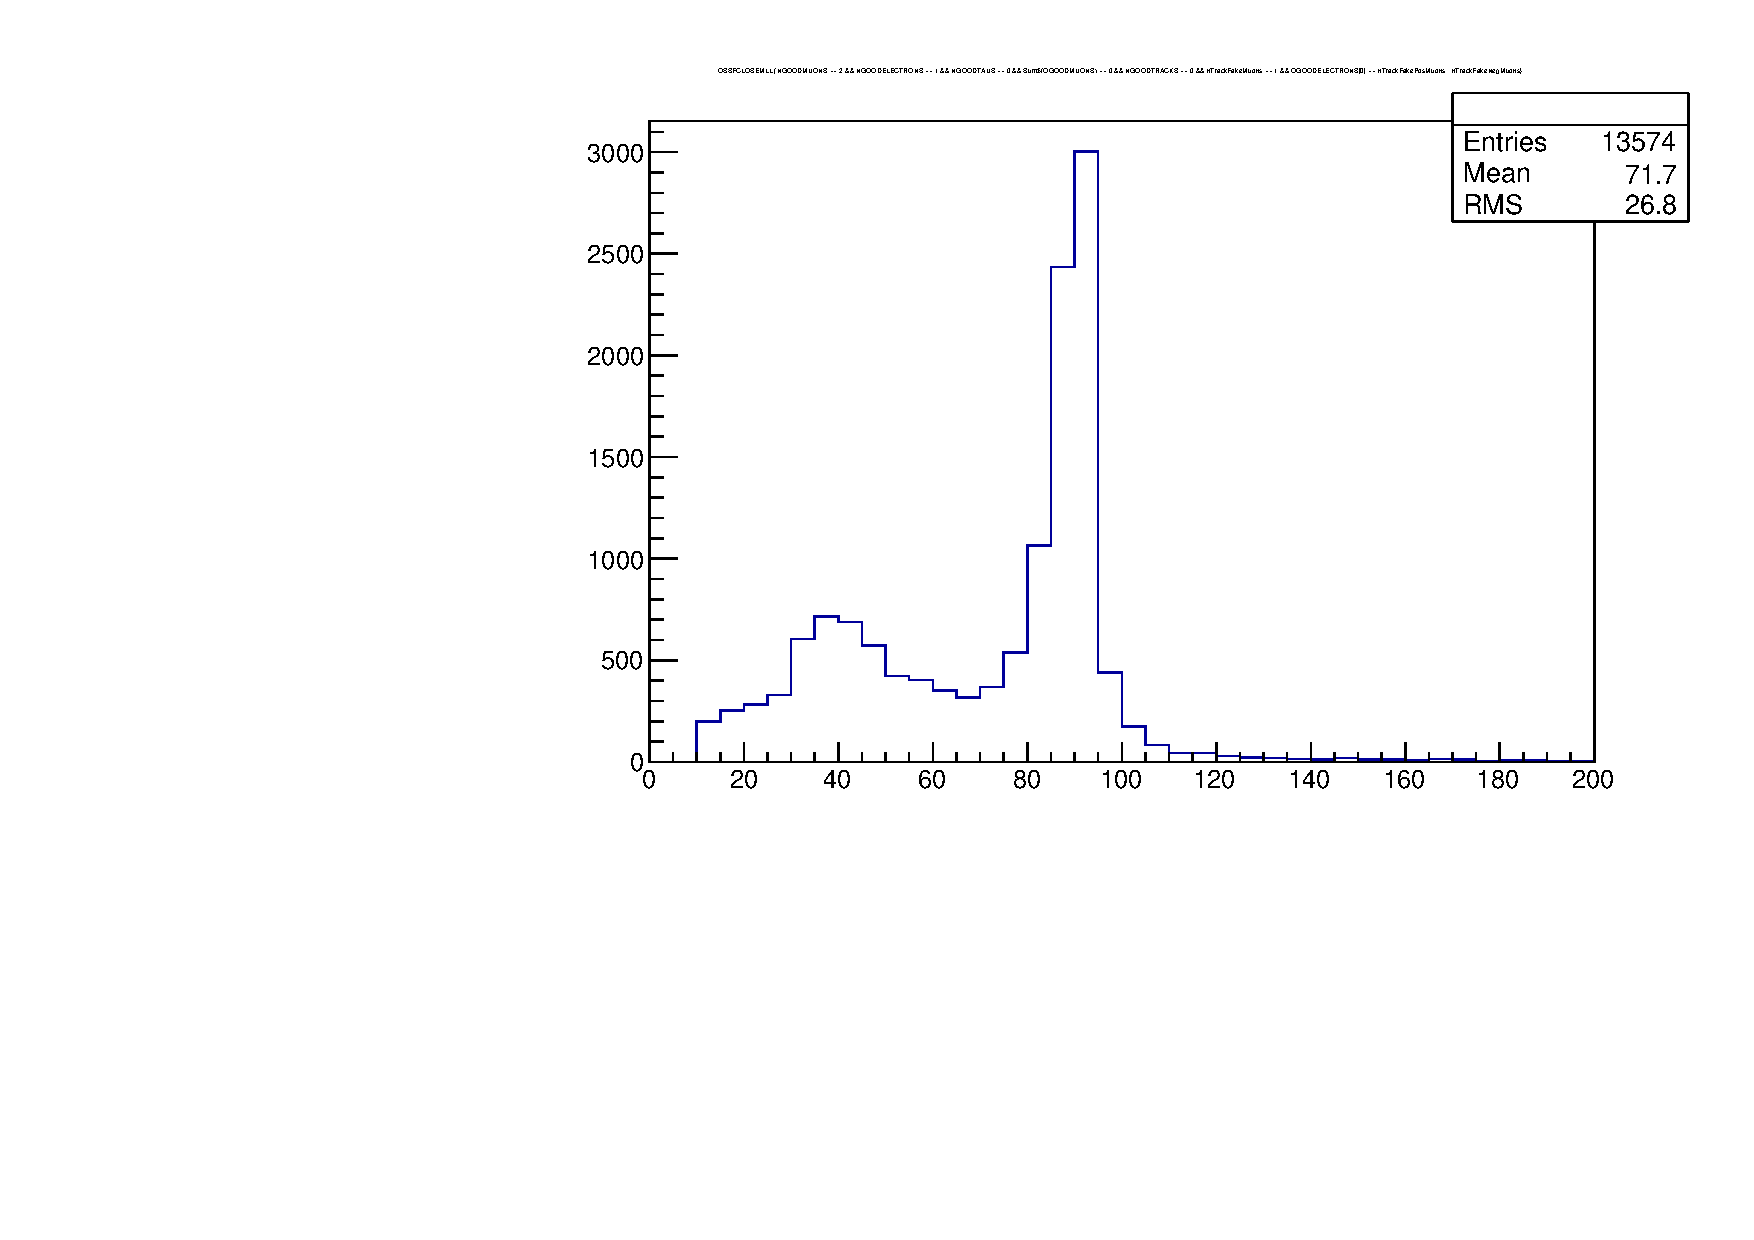
\includegraphics[width=.5\textwidth]{Appendix/study_OSSFCLOSEMLL_muon,track_1fake}%
	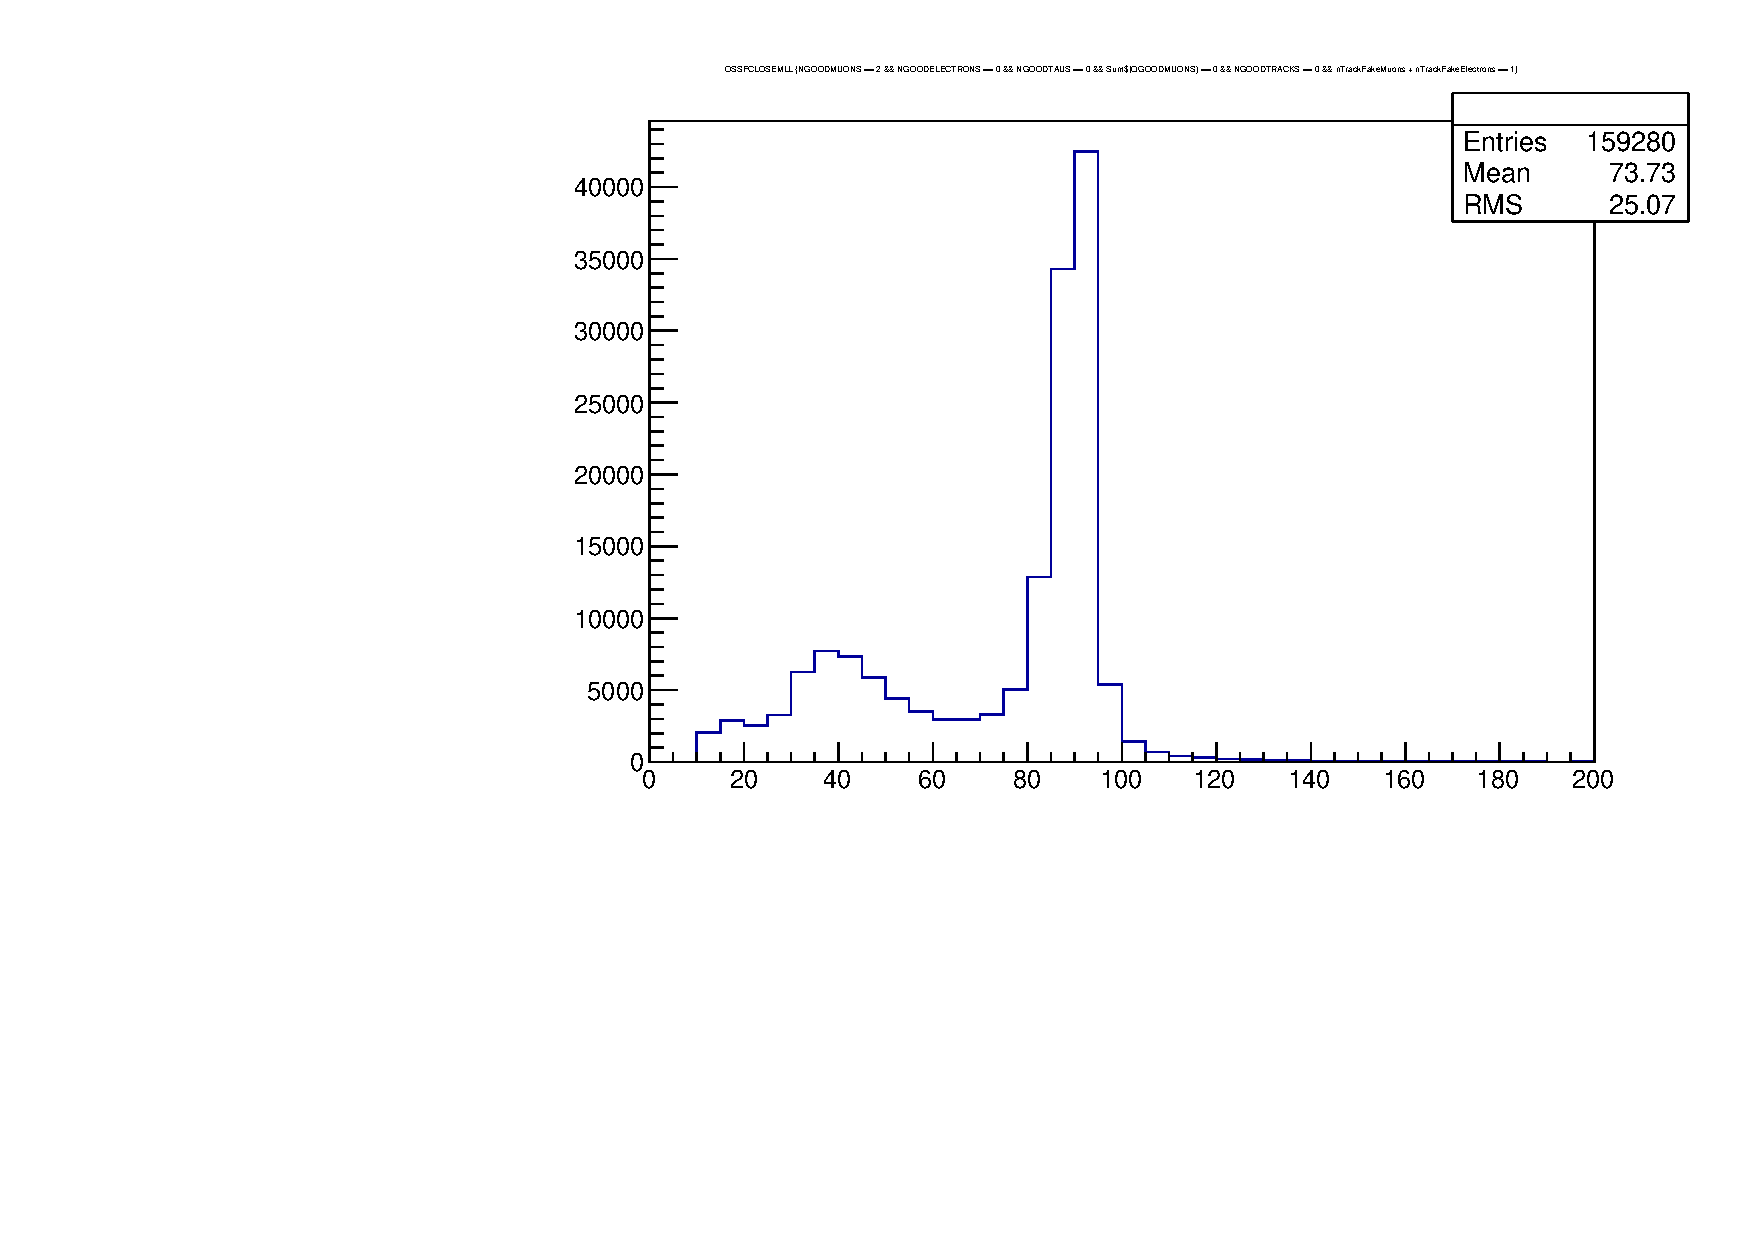
\includegraphics[width=.5\textwidth]{Appendix/study_OSSFCLOSEMLL_muon,track_dileptons-1fake}
	\caption{Top: $m_{et}$ distribution; bottom: $m_{\mu t}$ distribution. Left: no other leptons present, right: additional lepton present. If a third lepton is present, its flavor is opposite the flavor of the first lepton, and its charge is the same as the track's (rejecting third leptons from \Z).\\
	\textbf{Note:} This is from the dilepton-triggered dataset, i.e. the tracks used here probably were good enough leptons to trigger.
	\label{fig:app:MOSSFlepton,track}}
\end{center}
\end{figure}

This suggests that tracks are not only from jets, but also from low quality leptons. So, tracks do model fake leptons from jets, and at the same time also model leptons that were vetoed by quality cuts. However, the general shape of the track background is still expected to be in agreement with the shape of the signal regions. \fixme{Does that make sense? Also, understand the left--right difference in Figure~\ref{fig:app:MOSSFlepton,track}?}

\chapter{Relative Sensitivity of Signal Regions}
To get a feeling on how different signal regions contribute to the limit, we present the expected single-channel $r$-values for the top 10 channels in Table~\ref{tab:topSensitivity}, using the signal with $m_\Sigma = 420\,\GeV$.

\begin{table}[h]
\centering
\caption{Relative Sensitivity of Signal Regions} \label{tab:topSensitivity}
\caption*{DY0: no OSSF pair, DYz1: 1 pair on \Z,\\ DYh1: 1 pair above \Z, DYgt0: $\geq 1$ pair}
\begin{tabular}{l c}
\hline\hline
Signal region & $r_\textrm{exp}$\\
\hline
L3 DYh1 LTMET550to750 & 2.6953\\
L3 DY0 LTMET550to750 & 3.6094\\
L3 DYh1 LTMET750to950 & 4.0781\\
L4 DYgt0 LTMET550to750 & 4.1094\\
L4 DYgt0 LTMET750to950 & 5.5938\\
\hline
L3 DY0 LTMET750to950 & 5.8750\\
L3 DYh1 LTMET350to550 & 6.2500\\
L3 DYz1 LTMET550to750 & 6.7188\\
L3 DY0 LTMET350to550 & 7.5938\\
L3 DYh1 LTMET950to1150 & 8.7812\\
\end{tabular}
\end{table}

\chapter{Additional Information on Multi-Isolation}
\label{app:MultiIso}

\textbf{Note:} This section is taken verbatim from SUS-15-008 PAS \cite{CMS-PAS-SUS-15-008} (thanks to our colleagues!).

The charged leptons produced in decays of heavy particles, such as $\PW$ and $\cPZ$ bosons 
or SUSY particles, are typically spatially isolated from the hadronic activity in the event,
while the leptons produced in the decays of hadrons or misidentified leptons are usually
embedded in jets. This distinction becomes less evident moving to
highly boosted systems where decay products tend to overlap.
%Therefore, in order to discriminate between the signal and background leptons, 
Therefore, given the higher collision energy explored in this analysis, a new and improved isolation definition is constructed using three variables as input:

\begin{itemize}
\item A mini-isolation (\miniIso)~\cite{Rehermann:2010vq} which is computed as a ratio of the scalar sum of transverse momenta 
of the charged hadrons, neutral hadrons, and photons within a cone of radius $R (\pt^\ell)$ around the lepton 
candidate direction at the origin, to the transverse momentum of the candidate. The cone radius $R$
depends on lepton $\pt$ as 
 \begin{equation}
R(\pt^\ell) = \dfrac{10\GeV}{\min\left[\max\left(\pt^\ell, 50\GeV\right), 200\GeV\right]}.
  \end{equation}
%The impact of the particles from other collisions in the event (pile up) is mitigated 
The varying isolation cone definition takes into account the aperture of b hadron decays as a function of
their $\pt$, and reduces the inefficiency from accidental overlap between the lepton and jets 
in a busy event environment.
\item A ratio between the lepton $\pt^\ell$ and $\pt^\text{jet}$ of a jet containing the lepton: 
 \begin{equation}
\ptRatio = \dfrac{\pt^\ell}{\pt^\text{jet}}.
  \end{equation}
The \ptRatio variable acts as a relative isolation in 
a larger cone. It improves mini-isolation performance when there
are no nearby jets, expecially for low-$\pt$ leptons. %It helps to estimate level of lepton isolation for low-$\pt$ leptons.
\item Transverse momentum of the lepton relative to the residual momentum of the closest jet after lepton momentum subtraction:
  \begin{equation}
    \ptRel=\frac{(\vec{p}(\text{jet})-\vec{p}(\ell))\cdot \vec{p}(\ell) }{|\vec{p}(\text{jet})-\vec{p}(\ell)|}.
  \end{equation}
The \ptRel variable allows to identify leptons that accidentally overlap with other jets in the event.
\end{itemize}

A lepton is considered to be isolated if the following condition is respected:
\begin{equation}
  \miniIso < I_1 \wedge ( \ptRatio > I_2 \vee \ptRel > I_3 )
\end{equation}

The values of $I_\text{i}, i = 1,2,3,$ depend on the lepton flavor; as the probability to misidentify a lepton is higher for electrons, 
tighter isolation values are used in this case (see Table~\ref{tab:isoWPs}). 
%The \multiIso working point for loose leptons is 
%used for the selection of the control regions and leptons used to form a veto.
%----------------------------------------------------------------------------------------------------------------------------
\begin{table}[h]
  \begin{center}
    %\small
    \caption{\label{tab:isoWPs}Multi-isolation working points used in the analysis.}
    \begin{tabular}{l|c|c|c}
      \hline
      Isolation value & Loose leptons  & Tight muons & Tight electrons  \\
      \hline\hline
      $I_1$ & 0.4 & 0.16 & 0.12 \\
      $I_2$ & 0 & 0.76 & 0.80 \\
      $I_3 (\GeV)$ & 0 & 7.2 & 7.2 \\
      \hline
    \end{tabular}
  \end{center}
\end{table}
%----------------------------------------------------------------------------------------------------------------------------

\chapter{Back-of-the-Envelope Limits}

We derive a rough estimate of the r-values for the 200\,\GeV mass point manually to verify that our result is in the right ballpark. We first estimate the expected number of decays from the most significant processes, and then calculate back-of-the-envelope limits both for the sum of all channels, and for the DY0 channel alone. Numbers given in [] in the table headings refer to the numbered explanaitions underneath.

\subsection*{Expected number of decays from the most significant processes}

\begin{table}[h!]
\centering
\caption{Most significant contributing processes} %\label{tab:}
\begin{tabular}{lllll}
Process ID & Process                                         & Final state [1] & xsec*BR*kfactor [fb] [2] & Expected total Decays [3] \\
A          & $tr^\pm wvtr^0wl$ & $w^\pm w l$             & 344                              & 792                           \\
B          & $tr^\pm zltr^0wl$ & $z l w^\pm l$           & 172                              & 395                           \\
C          & $tr^\pm hltr^0wl$ & $h l w^\pm l$           & 143                              & 330                           \\
D          & $tr^+zltr^- zl$  & $z l z l$             & 42                               & 97                           
\end{tabular}
\end{table}

\begin{enumerate}
	\item Final state is from decays of fermion triplet tr+-/tr0. Makes no assumption on lepton type.
	\item K-factor is taken to be 1.44
	\item Expected total decays taken to be Column 3 with 2.3 fb-1 of luminosity.
\end{enumerate}


\subsection*{Expected number of reconstructed decays (all 3L channels)}

\begin{table}[h!]
\footnotesize
\centering
\caption{3L (e/mu) Reconstruction: Back of Envelope vs. Full Analysis} %\label{tab:}
\begin{tabular}{lllllll}
Process ID & Process       & BR 3 e/mu [1][2][3][4] & Expected 3(e/mu) [5] & Reconstructed [6] & Signal [7] & limit [8] \\
A          & $tr^\pm wvtr^0wl$ & $23\% \cdot 23\% \cdot 72\%$                         & 30.2                              & 19.9                                      & 16                                     &                                       \\
B          & $tr^\pm zltr^0wl$ & $72\% \cdot 72\% \cdot 23\%$                         & 47.1                              & 31                                        & 33.8                                   &                                       \\
C          & $tr^\pm hltr^0wl$ & $72\% \cdot 72\% \cdot 23\%$                         & 39.3                              & 25.9                                      & 28.2                                   &                                       \\
D          & $tr^+zltr^-zl$    & $16\% \cdot 72\% \cdot 72\%$                         & 8.1                               & 5.3                                       & 5.7                                    &                                       \\
           & SUM           &                                        & 124.6                             & 82                                        & 83.6                                   & 0.64                                 
\end{tabular}
\end{table}

\begin{enumerate}
	\item br(w$\to$e/mu)=23\% taking tau$\to$e/mu in account
	\item br(l$\to$e/mu)=72\% taking into account tau$\to$e/mu
	\item br(z$\to$e/mu) = 16\% taking into account tau$\to$e/mu
	\item z and h decays ignored if w is present
	\item Expected 3L (e/mu) events is final column on Slide 2, with 3L branching ratios present
	\item Assume 87\% lepton reconstruction efficiency in Back of Envelope calculations
	\item signal yield as estimate in our main analysis
	\item Final column is with 1900 BG events and a statistical factor of 3 from 95\% CL calculations
\end{enumerate}


\subsection*{Expected number of reconstructed decays (DY0 only)}

\begin{table}[h!]
\centering
\caption{DY0 region: Back of Envelope vs. Full Analysis} %\label{tab:}
\begin{tabular}{llllll}
Process ID & Process       & DY0 events [1] & Signal & 1/r-exp (manual) [2] & 1/r-exp (analysis) [3] \\
A          & $tr^\pm wvtr^0wl$ & 4.97                                & 4.16                     &                                   &                               \\
B          & $tr^\pm zltr^0wl$ & 7.75                                & 7.48                     &                                   &                               \\
C          & $tr^\pm hltr^0wl$ & 6.47                                & 8.23                     &                                   &                               \\
D          & $tr^+zltr^-zl$    & 0                                   & 0.55                     &                                   &                               \\
           & SUM           & 19.18                               & 20.42                    & 0.29                              & 0.28                         
\end{tabular}
\end{table}

\begin{enumerate}
	\item DY0 signal has a combinatoric factor of 1/4 from previous slide. ZZ processes cannot decay into DY0 state and hence this factor is 0 here.
	\item 1/r-exp in back of envelope calculations is for 4.8 expected and 4.8 observed for 20.4 signal (see Fig.~\ref{fig:limitEstimate}). 95\% CL is about 6
	\item Final column is from slide 30 of approval talk in exclusion plot. It is taken to be sigma-exp/sigma-theory
\end{enumerate}

\begin{figure}[h!]
\begin{center}
	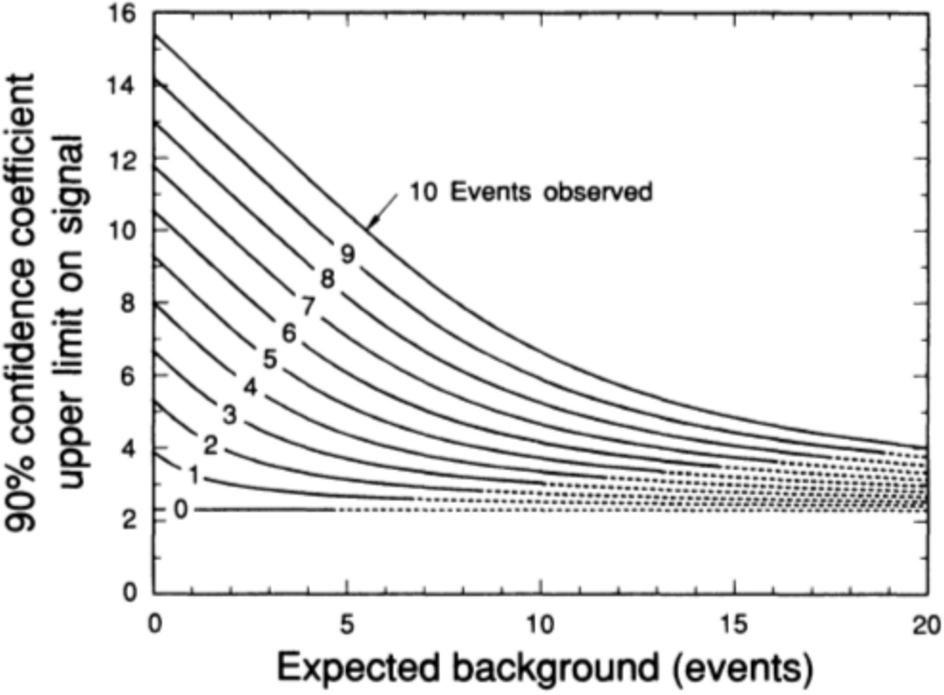
\includegraphics[width=.5\textwidth]{Appendix/limitEstimate}
	\caption{90\,\% CL upper limits as a function of the number of background events and the observation \cite{Hikasa:1992je}.
	\label{fig:limitEstimate}}
\end{center}
\end{figure}



\clearpage

\addcontentsline{toc}{chapter}{Bibliography}
\begin{singlespace}
\bibliographystyle{ieeetr}
\bibliography{thesis.bib}
\end{singlespace}

%%%%%%%%%%%%%%%%%% End of thesis %%%%%%%%%%%%%%%%%%
%\pagestyle{empty} % Using this removes last page number of the bibliography for unknown reasons

\end{document}
